%*******************************************************************************************
% File ini merupakan file template LaTEX untuk penulisan Disertasi pada Universitas Gunadarma Tahun 2018
%% Programmer  : Robby Kurniawan Harahap
%% E-mail  : robby_kurniawan@staff.gunadarma.ac.id
%% Pembuatan program template makalah ini dibuat dengan menggunakan :
%% Linux Opensuse Leap 42.3
%% texstudio versi 2.12.22 dan kile
%% TeX Live 2016/TeX Live for SUSE Linux
%% acrobat reader atau okular

%*******************************************************************************************

%berikut langkah-langkah untuk mendapatkan hasil akhir Disertasi
%================================================================
%Untuk pengguna texstudio (Linux dan Windows) :
% buka template, MainTemplateDisertasi.tex
% run compile atau tekan tombol f9 pada keyboard untuk mendapatkan hasil

%Untuk pengguna texmaker (Linux dan Windows):
% buka template, MainTemplateDisertasi.tex
% run compile untuk mendapatkan hasil

%Untuk pengguna kile:
% buka template, MainTemplateDisertasi.tex
% run compile PDFLatex untuk mendapatkan hasil

%berikut ini langkah-langkah untuk mendapatkan hasil akhir disertasi

%==============================================================
% Untuk platform Windows, berikut software yang diperlukan :
% 1. MiKTeX (Latex versi Windows). Dapat didownload dari situs http://miktex.org/
% 2. WinEdt (dapat didownload dari http://www.winedt.com
% 3. ghostscript
% 4. gimp untuk mengedit gambar
% 5. Adobe reader atau foxit reader

%==============================================================
% 
%  berikut ini langkah-langkah untuk mendapatkan hasil akhir disertasi menggunakan  WinEdt :
%  tekan tombol Latex
%  tekan tombol bibtex
%  tekan tombol makeindex
%  tekan tombol Latex
%  tekan tombol Latex
%  tekan tombol Pdf Latex/Pdf Texify
%=======================================================================================================
% jika terjadi masalah dalam penulisan silahkan hubungi programmer 
%% E-mail  : robby_kurniawan@staff.gunadarma.ac.id


\documentclass[a4paper,12pt,oneside]{disertasi}
\usepackage[a4paper,top=3cm,right=3cm,bottom=3cm,left=4cm]{geometry}
\usepackage[indonesia]{babel}
\usepackage[T1]{fontenc}
\usepackage[latin1]{inputenc}
\setcounter{secnumdepth}{3}
\setcounter{tocdepth}{3}
\setcounter{totalnumber}{4}
\usepackage{array}
\usepackage{multirow}
\usepackage{array,longtable}
\usepackage{graphicx}
\usepackage{epstopdf}
\usepackage{setspace}
\usepackage{multind}
\usepackage{rotating} %for rotate/sideway text
\usepackage{subfig} %for make floating sub-figure
\usepackage{natbib}
\usepackage{float}
\usepackage{lscape}
\usepackage{pseudocode}

\usepackage{lipsum}
\usepackage{fancyhdr}
\usepackage{amsmath}
\usepackage{enumerate}
\usepackage{enumitem}
\usepackage[table,xcdraw]{xcolor}
\usepackage{afterpage}
\usepackage{algorithmicx}
\usepackage{algcompatible}
\usepackage{algpseudocode}
\usepackage[
bookmarksopen,
bookmarksdepth=2,
breaklinks=true]{hyperref}
\hypersetup{
	colorlinks=true, % tadinya false
	linkcolor=black,
	citecolor=black,
	filecolor=black,
	%pagecolor=black,
	urlcolor=blue,
	bookmarks=true,
	pdfborder={0 0 0 0},
	pdftitle={MainTemplateDisertasi},
	pdfauthor={me},
	pdfkeywords={somekeywords},
	pdfdisplaydoctitle=true,
	pdftoolbar=true,
	pdfmenubar=true,
	pdfstartview=X Y Z
}
\usepackage{amssymb}% http://ctan.org/pkg/amssymb
\usepackage{pifont}% http://ctan.org/pkg/pifont
\usepackage{listings}
\usepackage{alltt}
%\usepackage[toc,page]{appendix} by sunny
\usepackage{multirow}
\usepackage{booktabs}
\usepackage{tabularx}
\usepackage[table]{xcolor}
\usepackage{longtable}
\hypersetup{breaklinks=true}
\usepackage{tikz}
%\usepackage{adjustbox}
\usepackage[hyphenbreaks]{breakurl}
\usepackage{etoolbox}
\usepackage{array, hhline}
\usepackage{colortbl}
\usepackage{lmodern}
\usepackage{color} %red, green, blue, yellow, cyan, magenta, black, white
\definecolor{mygreen}{RGB}{28,172,0} % color values Red, Green, Blue
\definecolor{mylilas}{RGB}{170,55,241}
\definecolor{darkblue}{rgb}{0,0,.75}
\usepackage{caption}
\usepackage{adjustbox} % auto adjust table

\usepackage[chapter]{algorithm}
\usepackage{makecell}
\usepackage{graphbox}

\usepackage{multicol}
\setlength{\columnsep}{0cm}

\usepackage{titlesec}
\titleformat{\chapter}[display]
{\normalfont\Large\bfseries\centering}{\centering\chaptertitlename\ \thechapter}{14pt}{\Large\bfseries}
\titlespacing*{\chapter}{0pt}{-30pt}{40pt}

\usepackage{textcomp}


\renewcommand{\thechapter}{\Roman{chapter}\bfseries}
\renewcommand{\thesection}{\arabic{chapter}.\arabic{section}}
%%\renewcommand{\thesubsection}{\arabic{chapter}.\arabic{section}.\arabic{subsection}}

\renewcommand{\thefigure}{\arabic{chapter}.\arabic{figure}}
\renewcommand {\thetable}{\arabic{chapter}.\arabic{table}} 
\renewcommand {\theequation} {\arabic{chapter}.\arabic{equation}} 

\renewcommand{\arraystretch}{1}
\renewcommand*{\arraystretch}{1}



\setcounter{chapter}{0}
\makeatletter

\lstset{language=Matlab,%
	%basicstyle=\color{red},
	breaklines=true,%
	morekeywords={matlab2tikz},
	keywordstyle=\color{blue},%
	morekeywords=[2]{1}, keywordstyle=[2]{\color{black}},
	identifierstyle=\color{black},%
	stringstyle=\color{mylilas},
	commentstyle=\color{mygreen},%
	showstringspaces=false,%without this there will be a symbol in the places where there is a space
	numbers=left,%
	numberstyle={\tiny \color{black}},% size of the numbers
	numbersep=9pt, % this defines how far the numbers are from the text
	emph=[1]{for,end,break},emphstyle=[1]\color{red}, %some words to emphasise
	%emph=[2]{word1,word2}, emphstyle=[2]{style},    
}



%%% Letakkan disini buat Appendice
\newcommand{\listofappendices}{\bgroup%
	\renewcommand\contentsname{DAFTAR LAMPIRAN}
	\let\@startoc@temp\@starttoc%
	\def\@starttoc##1{\@startoc@temp{app}}%
	\clearpage
	\tableofcontents \egroup
}

\let\oldemptyset\emptyset
\let\emptyset\varnothing

\newenvironment{conditions}
{\par\vspace{\abovedisplayskip}\noindent\begin{tabular}{>{$}l<{$} @{${}={}$} l}}
	{\end{tabular}\par\vspace{\belowdisplayskip}}


\newcommand*{\skipnumber}[2][1]{%
	{\renewcommand*{\alglinenumber}[1]{}\State #2}%
	\addtocounter{ALG@line}{-#1}}

\def\NoNumber#1{{\def\alglinenumber##1{}\State #1}\addtocounter{ALG@line}{-1}}


\renewcommand{\thealgorithm}{\arabic{chapter}.\arabic{algorithm}}
\renewcommand{\ALG@name}{Algoritma}
\renewcommand{\listalgorithmname}{DAFTAR ALGORITMA}

%Pseudocode
\newcounter{nalg}[chapter] % defines algorithm counter for chapter-level
\renewcommand{\thenalg}{\thechapter .\arabic{nalg}} %defines appearance of the algorithm counter
\DeclareCaptionLabelFormat{algocaption}{PseudoCode \thenalg}
\lstloadlanguages{Matlab} %use listings with Matlab for Pseudocode
\lstnewenvironment{PseudoCode}[1][]
{\lstset{language=Matlab,basicstyle=\scriptsize, keywordstyle=\color{darkblue},numbers=left,xleftmargin=.04\textwidth,#1}}
{}

\algrenewcommand{\algorithmicwhile}{\textbf{WHILE}}
\algrenewcommand{\algorithmicif}{\textbf{IF}}
\algrenewcommand{\algorithmicelse}{\textbf{ELSE}}
\algrenewcommand{\algorithmicthen}{\textbf{THEN}}
\algrenewcommand{\algorithmicend}{\textbf{END}}
\algrenewcommand{\algorithmicprocedure}{\textbf{PROCEDURE}}

\newcounter{algsubstate}
\makeatletter
\renewcommand{\thealgsubstate}{\arabic{ALG@line}.\alph{algsubstate}}
\makeatother
\newenvironment{algsubstates}
{\setcounter{algsubstate}{0}%
	\renewcommand{\State}{%
		\refstepcounter{algsubstate}%
		\Statex {\footnotesize\alph{algsubstate}:}\space}}


\newcommand{\abbrlabel}[1]{\makebox[3.5cm][l]{\textbf{#1}}}
\newenvironment{abbreviations}{\begin{list}{}{\renewcommand{\makelabel}{\abbrlabel}}}{\end{list}}




%% Bagian Pemenggalan Kata Yang Tidak Sempurna
\hyphenation{me-tode pe-rang-kat me-rekam ber-dasar-kan me-lakukan di-usul-kan di-antara-nya Ge-neration ci-tra Ci-tra pe-ngu-kur-an} 
%% kata yang dipenggal dengan tak sempurna

\renewcommand{\headrulewidth}{2pt}
%\renewcommand{\footrulewidth}{2pt}

\newenvironment{conditions*}
{\par\vspace{\abovedisplayskip}\noindent
	\tabularx{\columnwidth}{>{$}l<{$} @{${}={}$} >{\raggedright\arraybackslash}X}}
{\endtabularx\par\vspace{\belowdisplayskip}}
\doublespacing
\makeatother
\parindent 3.0em

% Renew the command that starts the appendices.
\usepackage{titlesec}
\renewcommand{\chaptername}{CHAPTER}
\titlespacing*{\chapter}{0pt}{0.45in}{0.3in}
\titleformat{\chapter}[display]
{\normalfont\Large\centering\bfseries}{\chaptertitlename\ \thechapter}{0pt}{\Large\uppercase}
\titleformat{\section}{\large\bfseries}{\thesection}{1em}{}










\begin{document}
	\nocite{*}
	%#start bagian administrasi #==================================================
	% bagian muka sebelum isi, umumnya halaman administrasi, kalau tidak digunakan
	% dapat diberikan tanda % didepannya
	%cover
	\pagestyle{empty}
	\pagenumbering{roman}
	\setcounter{page}{1}
	 \newpage
\addcontentsline{toc}{chapter}{COVER}
\begin{center}

\begin{figure}[h]
\begin{center}
\includegraphics[%
scale=0.6]{LogoGundar.eps}\end{center}
\end{figure}

\vspace{1.0cm}

 %{\fontsize{15.5}{48} \selectfont \textbf{Sistem Pemantauan Kualitas Gambar pada Siaran}}\\
 %{\fontsize{15.5}{48} \selectfont \textbf{Televisi Digital DVB-T2 berbasis Metrik Obyektif}}\\
 %{\fontsize{15.5}{48} \selectfont \textbf{yang Diukur secara Waktu Nyata}}
 {\fontsize{12}{15} \selectfont \textbf{PENGEMBANGAN METODE DETEKSI DAN MENGHITUNG JUMLAH POHON KELAPA SAWIT DARI SENTINEL 2 IMAGERY MENGGUNAKAN METODE \textit{OBJECT-BASED IMAGE ANALYSIS} (OBIA)}}\\

 
%\vfill
\vspace{3cm}
{\large DISERTASI}
\vspace{2cm}



%\vfill
\vspace{1cm}
{\large \underline{\textbf{GUNTUR EKA SAPUTRA}}\\
\vspace{0.1cm}99219009}


%\vfill
\vspace{2.5cm}

{\fontsize{12}{48} \selectfont \textbf{PROGRAM DOKTOR TEKNOLOGI INFORMASI}}% \vspace{0.1cm}

{\fontsize{12}{48} \selectfont \textbf{UNIVERSITAS GUNADARMA}} % \vspace{0.1cm}

{\fontsize{12}{48} \selectfont \textbf{2023}}

\end{center} 
	\pagestyle{plain}
	\pagenumbering{roman}
	\setcounter{page}{2}
	\newpage
\addcontentsline{toc}{chapter}{HALAMAN JUDUL}

\begin{center}

\begin{figure}[h]
\begin{center}
\includegraphics[%
  scale=0.6]{LogoGundar.eps}\end{center}
\end{figure}

\vspace{1.0cm}
%{\fontsize{15.5}{48} \selectfont \textbf{Sistem Pemantauan Kualitas Gambar pada Siaran}}\\
%{\fontsize{15.5}{48} \selectfont \textbf{Televisi Digital DVB-T2 berbasis Metrik Obyektif}}\\
%{\fontsize{15.5}{48} \selectfont \textbf{yang Diukur secara Waktu Nyata}}
{\fontsize{12}{48} \selectfont \textbf{Pengembangan Metode Deteksi Dan Menghitung Jumlah Pohon Kelapa Sawit Dari Sentinel 2 Imagery Menggunakan Metode \textit{OBJECT-BASED IMAGE ANALYSIS} (OBIA)}}\\


%\vfill
%\vspace{1.5cm}
\vspace{1cm}

{\large DISERTASI}

\vspace{0.5cm}

Untuk Memenuhi Salah Satu Syarat Meraih Gelar Doktor Teknologi Informasi di bawah Pimpinan Rektor Universitas Gunadarma \\ Profesor Doktor E.S. Margianti, SE, MM

\vspace{1.5cm}

Laporan Rapat Komisi Pembimbing
Dipertahankan dalam Sidang Terbuka Senat Universitas Gunadarma\\
Pada Hari Rabu, 10 Mei 2023

%\vspace{1.5cm}
\vspace{1cm}

{\large \underline{\textbf{{GUNTUR EKA SAPUTRA}}}\\

 \vspace{0.1cm}\textbf{99219009}}

%\vfill

\vspace{1cm}


{\fontsize{12}{48} \selectfont \textbf{PROGRAM DOKTOR TEKNOLOGI INFORMASI}}% \vspace{0.1cm}
% \fontsize{14}{48} \selectfont \textbf{PROGRAM PASCASARJANA}\\ % \vspace{0.1cm}

{\fontsize{12}{48} \selectfont \textbf{UNIVERSITAS GUNADARMA}} % \vspace{0.1cm}

{\fontsize{12}{48} \selectfont \textbf{2023}}

\end{center} 

	
	%halaman lembar pengesahan, abstraksi, kata pengantar
	%nilai halaman utk awal dari abstrak s/d ucapan terimakasih dlm romawi
	\newpage
\addcontentsline{toc}{chapter}{LEMBAR PERSETUJUAN}


\begin{center}
	
	%\textbf{{\fontsize{14}{15}\selectfont Sistem Pemantauan Kualitas Gambar pada Siaran}}\\
	%\textbf{{\fontsize{14}{15}\selectfont Televisi Digital DVB-T2 berbasis Metrik Obyektif}}\\
	%\textbf{{\fontsize{14}{15}\selectfont yang Diukur secara Waktu Nyata}}\\
	\textbf{{\fontsize{12}{15}\selectfont PENGEMBANGAN METODE DETEKSI DAN MENGHITUNG JUMLAH POHON KELAPA SAWIT DARI SENTINEL 2 IMAGERY MENGGUNAKAN METODE \textit{OBJECT-BASED IMAGE ANALYSIS} (OBIA)}}\\
	
 
	%\vspace{1cm}
	\vspace{2cm}
	
	\textbf{{\normalsize DISERTASI}}
	
	%\vspace{1cm}
	\vspace{2cm}
	
	\textbf{{\normalsize GUNTUR EKA SAPUTRA}}
	
	
	
	%\vspace{1cm}
	\vspace{2cm}
		
	%Telah disetujui oleh:
	\textbf{Telah disetujui oleh:}
	
	%\vspace{2.5cm}
	\vspace{2cm}
	
	{\bf Profesor Doktor Insinyur Kudang Boro Seminar, M.Sc.}\\
	Promotor
	
	%\vspace{2.5cm}
	\vspace{2cm}
	
	{\bf Profesor Doktor Sarifuddin Madenda, S.Si., DEA.}\\
	Ko-Promotor
	
	%\vspace{2.5cm}
	\vspace{2cm}
	
	%{\bf Dr. Yulisdin Mukhlis}\\
	%Ko-Promotor\\
	%\vspace{1.5cm}
	Jakarta, 10 Mei 2023
	
\end{center}
	\newpage
\addcontentsline{toc}{chapter}{LEMBAR PENGUJI}

\hspace{-1.4cm}\begin{tabular}{llp{10cm}}
	Judul Disertasi & : & \textbf{PENGEMBANGAN METODE DETEKSI DAN MENGHITUNG JUMLAH POHON KELAPA SAWIT DARI SENTINEL 2 IMAGERY MENGGUNAKAN METODE \textit{OBJECT-BASED IMAGE ANALYSIS} (OBIA)}  \\
	&  & \\
	Nama Mahasiswa & : & Guntur Eka Saputra \\
	NIM  & : & 99219009\\
	&  & \\
	Komite Pembimbing &  & \\
	Promotor & : & Profesor Doktor Insinyur Kudang Boro Seminar, M.Sc.  \\
	Ko-Promotor & : &  Profesor Doktor Sarifuddin Madenda, S.Si., DEA.\\
	&  & \\
	Komite Penguji &  & \\
	Ketua  & : & Profesor Doktor Insinyur Kudang Boro Seminar, M.Sc.  \\ 
	&  & \\
	Anggota& : & Profesor Doktor Insinyur Sudrajat, M.Sc.\\
	&  &Profesor Doktor E. S. Margianti, S.E., M.M.\\
	&  &Profesor Suryadi Harmanto, S.Si., M.M.S.I.\\
	&  &Profesor Doktor Insinyur Bambang Suryawan, M.T.\\
	&  &Profesor Insinyur Busono Soerowirdjo, M.Sc., Ph.D.\\
	&  &Profesor Doktor Eri Prasetyo Wibowo, S.Si., M.M.S.I.\\
	&  &Doktor rer. nat. I Made Wiryana, S.Si., S.Kom., M.App.Sc.\\
	&  &Doktor Detty Purnamasari, S.Kom., M.M.S.I., M.I.Kom.\\
	&  &Profesor Doktor Sarifuddin Madenda, S.Si., D.E.A.\\

\end{tabular}




  













	\newpage %Acknowledgment
\addcontentsline{toc}{chapter}{PERNYATAAN ORIGINALITAS DAN PUBLIKASI}
\begin{center}
\begin{large}\textbf{PERNYATAAN ORIGINALITAS DAN PUBLIKASI}\\\end{large}
\end{center}
\vspace{1cm}
\begin{flushleft}
  Saya yang bertanda tangan di bawah ini:

\hspace{-0.2cm}\begin{tabular}{llp{10cm}}
  Nama & : & Guntur Eka Saputra\\
  NIM & : & 99219009 \\
    & &  \\
    
  Judul Disertasi & : & PENGEMBANGAN METODE DETEKSI DAN MENGHITUNG JUMLAH POHON KELAPA SAWIT DARI SENTINEL 2 IMAGERY MENGGUNAKAN METODE \textit{OBJECT-BASED IMAGE ANALYSIS} (OBIA) \\
   & &  \\
    & &  \\
    Tanggal Sidang & : & 10 Mei 2023\\
    Tanggal Lulus & : & 10 Mei 2023\\
\end{tabular}


%\begin{tabbing}
% \hspace{4cm}\=\kill
%  Nama\>: Nama Mahasiswa\\
%  NPM\>: NPM \\
%  \> \\
%   Judul Disertasi\>: \textbf{Judul Disertasi Baris 1} \\
%\> ${}$\hspace{0.65em}\textbf{Judul Disertasi Baris 2} \\
%\> ${}$\hspace{0.65em}\textbf{Judul Disertasi Baris 3} \\
%
%
%
%
%
%Tanggal Sidang \>: Tanggal Sidang\\
%Tanggal Lulus \>: Tanggal LULUS \\
%\end{tabbing}
%
%



\end{flushleft}
Menyatakan bahwa tulisan ini adalah merupakan hasil karya saya sendiri dan dapat dipublikasikan sepenuhnya oleh Universitas Gunadarma. Segala kutipan dalam bentuk apapun telah mengikuti kaidah dan etika yang berlaku. Mengenai sisi dan tulisan adalah merupakan tanggung jawab Penulis, bukan Universitas Gunadarma.

Demikian pernyataan ini dibuat dengan sebenarnya dan dengan penuh kesadaran.
\vspace{0.5 cm}
\begin{flushleft}

Jakarta, 10 Mei 2023%% Tahun penulisan

\vspace{2.5 cm}
(Guntur Eka Saputra)
\end{flushleft} % menggabungkan file lembar pengesahan
	\newpage %Abstract
\addcontentsline{toc}{chapter}{ABSTRAK}
\begin{center}
%\begin{large}\textbf{Deteksi dan Klasifikasi Karies Molar Rahang Bawah Menggunakan Citra Radiograf Periapikal Gigi dengan Segmentasi Region Growing}\end{large}\\
%%\begin{large}\textbf{JUDUL DISETASI baris 2}\end{large}\\
\vspace{10mm}
\begin{large}\textbf{ABSTRAK}\end{large}
\end{center}
\vspace{5mm}

\begin{singlespace}
Penerapan teknologi informasi dan komunikasi sangat dibutuhkan,\\khususnya di bidang pertanian. Kelapa sawit merupakan produk pertanian yang terbesar di Indonesia dan produksi kelapa sawit sangat penting bagi perekonomian. Dalam menghasilkan produksi kelapa sawit yang baik dibutuhkan pengelolaan perkebunan kelapa sawit yang baik. Permasalahan utama dalam pengelolaan ini, yaitu luas area dalam skala besar (perusahaan perkebunan kelapa sawit memiliki luas mininimum sebesar 6.000 hektar yang harus dikelola), wilayah perkebunan berada di \textit{remote area}, akses infrastruktur yang terbatas, dan pemupukan presisi mengalami kesulitan untuk mendapatkan data secara akurat berdasarkan jumlah tegakkan pohon kelapa sawit pada suatu area lahan. Hal ini menyebabkan deteksi dan menghitung pohon kelapa sawit sangat dibutuhkan. Selama ini, penghitungan tradisional didasarkan pada catatan awal penanaman pohon kelapa sawit atau penghitungan teoritis berdasarkan jarak tanam antara pohon kelapa sawit dalam satu hektar atau blok. Metode tradisional ini lambat dan tidak akurat, serta tidak diketahui status pohon kelapa sawit yang rusak atau mati. Penggunaan teknologi dibutuhkan untuk dapat secara otomatis dan \textit{real-time} dalam memonitoring data pohon kelapa sawit dan memperkirakan produktivitasnya. Penggunaan ini dibutuhkan dalam deteksi objek berupa citra.

Penggunaan citra untuk deteksi objek dibutuhkan dalam persiapan data, seperti menganalisa, memberikan anotasi atau kelas dari objek tersebut. Metode dalam melakukan anotasi dataset selama ini dilakukan secara manual, satu per satu dengan memberikan kotak batas. Persiapan data ini menghabiskan lebih dari 70\% waktu dalam siklus hidup \textit{deep learning} untuk menjadi dataset yang dapat digunakan sebagai data pelatihan, validasi, dan pengujian. Hal inilah yang menjadi tantangan bagi \textit{stakeholders}. 

Penelitian ini bertujuan untuk menghasilkan pengembangan metode \textit{object-based image analysis} (OBIA) untuk membuat dataset secara otomatis dengan memberikan label suatu kelas pada data citra. Metode yang dikembangkan menggunakan algoritma klasifikasi \textit{template matching}. Algoritma ini sebagai template awal citra pohon kelapa sawit yang memiliki kunci nilai ambang batas dalam menentukan kelas dari objek di dalam citra. Algoritma BIRCH digunakan untuk mengurangi objek yang bukan terdeteksi ke dalam kelas pohon kelapa sawit. Hasil evaluasi performance pelatihan menunjukkan bahwa model dengan algoritma YOLOv7 lebih baik dengan akurasi best MAP sebesar 0,993 dan pada pengujian sebesar 0,997. Berdasarkan waktu pemrosesan DGX-A-100 Universitas Gunadarma lebih baik, pada pelatihan sebesar 2948 detik dibandingkan dengan Google Colab Pro sebesar 4847 detik.

Penelitian ini dihasilkan purwarupa sistem yang menggunakan model algoritma dari YOLOv7 untuk dapat mendeteksi dan menghitung pohon kelapa sawit pada area tertentu dari citra satelit yang terintegrasi dengan Google Maps API. Berdasarkan hasil pengujian 4 blok pada Kebun Pendidikan dan Pendidikan Kelapa Sawit IPB-Cargil bahwa hasil presentasi berhasil dideteksi sebesar 97,67\%, dan diketahui setiap pohon kelapa sawit yang terdeteksi diketahui letak titik koordinat untuk dapat dilakukan pemantauan, pengelolaan, dan estimasi produktivitas pohon kelapa sawit.

\end{singlespace}
\noindent \\

\noindent Kata kunci : OBIA, \textit{Deep Learning}, YOLOv7, Kelapa Sawit.% menggabungkan file abstraksi
	\newpage %Abstract
\addcontentsline{toc}{chapter}{ABSTRACT}
\begin{center}
%\begin{large}\textbf{Detection and Classification of Lower Molar Caries Using Dental Periapical Radiographic Image with Region Growing Segmentation  }\end{large}\\
 
 

\vspace{10mm}
\begin{large}\textbf{ABSTRACT}\end{large}
\end{center}
\vspace{5mm}

\begin{singlespace}
The application of information and communication technology is needed, especially in agriculture. Palm oil is the largest agricultural product in Indonesia and palm oil production is very important for the economy. In producing good oil palm production, good oil palm plantation management is needed. The main problems in this management, namely large-scale areas (oil palm plantation companies have a minimum area of 6,000 hectares that must be managed), plantation areas in remote areas, limited infrastructure access, and precision fertilization have difficulty obtaining accurate data based on the number of standing oil palm trees in a land area. This makes detecting and counting oil palm trees necessary. So far, traditional counting has been based on early records of oil palm tree planting or theoretical counting based on the spacing between oil palm trees within a hectare or block. These traditional methods are slow and inaccurate, and the status of damaged or dead oil palm trees is unknown. The use of technology is needed to be able to automatically and real-time monitor palm oil tree data and estimate its productivity. This use is needed in object detection in the form of images.

The use of images for object detection is needed in data preparation, such as analyzing, annotating or classifying the object. The method of annotating datasets has been done manually, one by one by providing boundary boxes. This data preparation consumes more than 70\% of the time in the deep learning lifecycle to become a dataset that can be used as training, validation, and testing data. This is the challenge for stakeholders.

This research aims to produce the development of object-based image analysis (OBIA) method to create datasets automatically by labeling a class on image data. The developed method uses a template matching classification algorithm. This algorithm as an initial template of palm tree image that has a key threshold value in determining the class of objects in the image. The BIRCH algorithm is used to reduce objects that are not detected into the palm tree class. The results of the training performance evaluation show that the model with the YOLOv7 algorithm is better with a best MAP accuracy of 0.993 and on testing of 0.997. Based on processing time, Gunadarma University's DGX-A-100 is better, at 2948 seconds of training compared to Google Colab Pro at 4847 seconds.

This research produced a prototype system that uses the algorithm model from YOLOv7 to be able to detect and count oil palm trees in a certain area from satellite images integrated with the Google Maps API. Based on the results of testing 4 blocks in the IPB-Cargil Oil Palm Education and Education Plantation that the presentation results were successfully detected by 97.67\%, and it is known that each detected oil palm tree is known to the location of the coordinate point to be able to monitor, manage, and estimate the productivity of oil palm trees.
\end{singlespace}

\noindent \\

\noindent Key words: OBIA, Deep Learning, YOLOv7, Oil Palm.
	\newpage %Acknowledgment
\addcontentsline{toc}{chapter}{KATA PENGANTAR}
\begin{center}
\begin{large}\textbf{KATA PENGANTAR}\\\end{large}
\end{center}
\vspace{5mm}
 

\textit{Bismillahhirrohmaanirrohim}

\textit{Assalamu'alaikum Warahmatullahi Wabarakatuh} 

\textit{Alhamdulillah robil'aalamin} 

Segala Puji, Kebesaran, Kemulian, dan apa yang dilangit dan di bumi milik Allah SWT. Puji Syukur saya panjatkan kehadirat Allah SWT atas segala rahmat serta nikmat-Nya yang telah memberikan kemudahan serta kelancaran kepada Saya dalam penyelesaian Disertasi yang berjudul "Pengembangan Metode Deteksi Dan Menghitung Jumlah Pohon Kelapa Sawit Dari Sentinel 2 Imagery Menggunakan Metode \textit{OBJECT-BASED IMAGE ANALYSIS} (OBIA)". Disertasi ini merupakan syarat untuk memperoleh gelar Doktor dalam bidang Teknologi Informasi pada Program Doktor Teknologi Informasi, Program Pascasarjana, Universitas Gunadarma, dimana penulis telah menyelesaikan seluruh rangkaian proses studi Program Doktor sejak tahun 2019. Sepanjang proses penyusunan Disertasi ini, banyak pihak yang turut membantu baik secara moril maupun materil kepada saya. Untuk itu dengan segala kerendahan dan ketulusan hati, perkenankan saya mengucapkan terima kasih kepada:


\begin{enumerate}

%\item Yayasan Pendidikan Gunadarma, yang telah memberikan beasiswa studi di Program Doktor Teknologi Informasi Universitas Gunadarma.
%\item Ibu Prof. Dr. E.S. Margianti, S.E., MM., selaku Rektor Universitas Gunadarma.
%\item Bapak Prof. Suryadi Harmanto, SSi., MMSI., selaku Pembantu Rektor II Universitas Gunadarma.
%\item Bapak Prof. Dr. Ir. Bambang Suryawan, MT., selaku Koordinator Program Pasca Sarjana Universitas Gunadarma.
%\item Bapak Prof. Ir. Busono Soerowirdjo, MSc., PhD., selaku Direktur Program Doktor Universitas Gunadarma sekaligus Promotor diselasela kesibukannya dengan sabar membimbing, mengarahkan, memberi masukan dan memotivasi dalam menyelesaikan disertasi.
%\item Bapak Prof. Dr. Sarifuddin Madenda, selaku Ketua Program Doktor Teknologi Informasi Universitas Gunadarma 
%\item Bapak Prof. Dr. Eri Prasetyo Wibowo, selaku Sekretaris Program Doktor Teknologi Informasi Universitas Gunadarma.
%\item Bapak -. selaku penguji luar yang telah berkenan menguji dan membrikan saran-saran serta arahan yang bermanfaat untuk perbaikan penulisan disertasi ini.
%\item Bapak Dr. Tubagus Maulana Kusuma selaku Ko-Promotor yang dengan sabar memberikan motivasi, koreksi, masukkan dan saran dalam menyelesaikan disertasi ini.
%\item Bapak Dr. Yulisdin Mukhlis selaku Ko-Promotor yang dengan sabar memberikan motivasi, koreksi, masukkan dan saran dalam menyelesaikan disertasi ini.
%\item Rekan-rekan dari Technology Development UG-Technopark, Yogi Permadi., dan Dhatu Paragya yang motivasi dalam menyelesaikan disertasi ini.
%\item Istri tercinta, Yuzeli Media  dengan penuh kesabaran mendampingi dan memberikan doa terbaik serta motivasi secara dalam proses penyelesaian disertasi ini.
%\item Ayahanda tercinta Suntiyono dan Ibunda tercinta Kastiyah yang selalu memberikan doa yang terbaik serta motivasi kepada penulis baik moril dan materiil.
\item Ibu Profesor Doktor E. S. Margianti, S.E., MM., selaku Rektor Universitas Gunadarma.
\item Bapak Profesor Doktor Insinyur Bambang Suryawan, MT., selaku Koordinator Program Pascasarjana Universitas Gunadarma.
\item Bapak Profesor Insinyur Busono Soerowirdjo, MSc., Ph.D., selaku Direktur Program Doktor Universitas Gunadarma.
\item Profesor Doktor Sarifuddin Madenda, selaku Ketua Program Doktor Teknologi Informasi Universitas Gunadarma sekaligus Ko-Promotor diselasela kesibukannya dengan sabar membimbing, mengarahkan, memberi masukan dan memotivasi dalam menyelesaikan disertasi
\item Bapak Profesor Doktor Eri Prasetyo Wibowo, selaku Sekretaris Program Doktor Teknologi Informasi Universitas Gunadarma.
\item Bapak Profesor Doktor Insinyur Kudang Boro Seminar, M.Sc. selaku Promotor yang dengan sabar memberikan membimbing, memotivasi, melakukan koreksi, memberi masukkan dan saran dalam menyelesaikan disertasi ini.
\item Bapak Profesor Doktor Insinyur Sudrajat, M.Sc., selaku Penguji Luar terima kasih atas waktu, kesediaan, dan masukkan, serta saran disertasinya bagi saya.
\item Bapak Profesor Suryadi Harmanto, SSi., MMSI, Bapak Doktor rer. nat. I Made Wiryana dan Ibu Doktor Detty Purnamasari selaku penguji dalam yang telah memberi banyak masukan dan saran perbaikan, sehingga disertasi ini semakin berkualitas.
\item Bapak Doktor Irwan Bastian yang telah memberikan dukungan kepada saya dapat melaksanakan kuliah Program Doktor Teknologi Informasi di Universitas Gunadarma.
\item Ayahanda tercinta Baikusnendro dan Ibunda tercinta Mennik Trihastuti, yang selalu memberikan doa yang terbaik dan motivasi, serta kedua adik saya Finsa Dwi Hestu Fikriansya, dan Hilmi Hestu Saputra yang selalu mendukung secara moril.
\item Rekan-rekan angkatan 25 Program Doktor Teknologi Informasi Universitas
Gunadarma yang selalu memberikan semangat, dan Mas Bonang Waspadadi Ligar, serta Sumaiyah Fitriandini yang berjuang bersama, serta diskusi.
\item Ibu-ibu di Sekretariat Program Doktor Teknologi Informasi Universitas Gunadarma Ibu Doktor Diny Wahyuni, Ibu Doktor Reni Diah Kusumawati, Ibu Doktor Aini Suri Talita, dan Ibu Doktor Dety Purnamasari yang sangat membantu dalam administrasi penyelesaian disertasi ini.
\item Teman-teman Bidang Kemahasiswaan Universitas Gunadarma, komunitas GDSC UG, Gunadarma IO, UGTV, Tim Teknis UG dan sahabat saya Muhammad Rifqi Al Furqon, Manfred Michael, dan Evan Sakti Endi yang telah membantu dalam penyelesaian disertasi ini.
\end{enumerate}

Semoga Allah SWT memberikan limpahan kebaikan dan pahala atas semua perhatian dan dukungan yang Bapak, Ibu, Saudara sekalian berikan kepada saya. Harapan saya agar Disertasi ini memberikan manfaat nyata bagi semua pihak yang berkepentingan. Saya mengharapkan kritik dan saran untuk perbaikan pada masa yang akan datang.


\begin{flushleft}
\textit{Wassalamu'alaikum Warahmatullahi Wabarakatuh}
\end{flushleft}

\begin{flushleft}
Jakarta, 10 Mei 2023\\
%Penulis
\vspace{2.5 cm}
(Guntur Eka Saputra)

\end{flushleft} 
% mengabungkan file kata pengantar
	%# akhir bagian administrasi # ==================================================
	 
     
            
	% #mulai membuat daftar isi, daftar gambar dan  daftar tabel # ========================
	%\setcounter{page}{8} %set nilai halaman sesuai urutannya
	\newpage
\addcontentsline{toc}{chapter}{DAFTAR ISTILAH}
\singlespacing

\begin{center}
	\begin{large}\textbf{DAFTAR ISTILAH}\end{large}
\end{center}
\vspace{1cm}


\noindent \begin{large}\textbf{Akronim}\end{large}
	\begin{abbreviations}
		\item[ASIC] Application Specific Integrated Circuit
		\item[CAD] Computer Aided Design
		\item[EDA] Electronic Design Automation
		
	\end{abbreviations}
	
	
	\vspace{1cm}
	\noindent \begin{large}\textbf{Singkatan}\end{large}
	\begin{abbreviations}
		\item[AMS] Austria Micro System
		\item[CMOS] Complementary Metal Oxide Silicon
		\item[FPGA] Field Programmable Gate Array
		\item[GDSII] Graphics Data Station Information Interchang
		\item[HDL] Hardware Description Language
		\item[IP] Intellectual Property
		\item[IC] Integrated Circuit
		\item[$\mu$m] Mikrometer, $1 \times 10^{-6}$
		\item[RTL] Register Transfer Level
		\item[SOC] System On CHIP
		\item[VHDL] VHSIC Hardware Description Language
		\item[VHSIC] Very High Speed Interated Circuit
		\item[VLSI] Very Large Scale Integration
	\end{abbreviations}


	\vspace{1cm}
	\noindent \begin{large}\textbf{Simbol}\end{large}
	\begin{abbreviations}
		\item[AMS] Austria Micro System
		\item[CMOS] Complementary Metal Oxide Silicon
		\item[FPGA] Field Programmable Gate Array
		\item[GDSII] Graphics Data Station Information Interchang
		\item[HDL] Hardware Description Language
		\item[IP] Intellectual Property
		\item[IC] Integrated Circuit
		\item[$\mu$m] Mikrometer, $1 \times 10^{-6}$
		\item[RTL] Register Transfer Level
		\item[SOC] System On CHIP
		\item[VHDL] VHSIC Hardware Description Language
		\item[VHSIC] Very High Speed Interated Circuit
		\item[VLSI] Very Large Scale Integration
	\end{abbreviations}%
	% membuat daftar isi
	\addcontentsline{toc}{chapter}{DAFTAR ISI}
	\doublespacing
	\tableofcontents

	%% membuat daftar tabel
	\doublespacing
	\listoftables
	\addcontentsline{toc}{chapter}{DAFTAR TABEL}
	
	%membuat daftar gambar
	\doublespacing
	\listoffigures
	\addcontentsline{toc}{chapter}{DAFTAR GAMBAR}%masih masalah
	
	%membuat daftar algoritma
	\doublespacing
	\addcontentsline{toc}{chapter}{DAFTAR ALGORITMA}
	\listofalgorithms
	%\addcontentsline{toc}{chapter}{DAFTAR PSEUDOCODE}
	%\apptoc
	%\listofappendices
	%\addcontentsline{toc}{chapter}{DAFTAR LAMPIRAN}
	%\listofappendices
	%%\newpage %lampiran
%\addcontentsline{toc}{chapter}{DAFTAR LAMPIRAN}
\begin{center}
\begin{large}\textbf{LAMPIRAN}\\\end{large}
\end{center}
%\vspace{5mm} Lampiran 1 Listing Program
%...............................................................................
%10

%%%%%%%%%%%%%%%%%%%%%%%%%% GAMBAR %%%%%%%%%%%%%%%%%%%%%%%%%%%%%%
\begin{figure}[H]
	\vspace{-0.1cm}
	%\rule{\columnwidth}{0.1pt}
	\begin{center}
		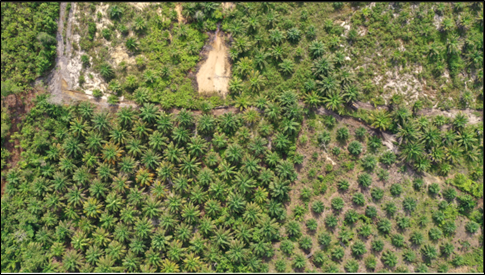
\includegraphics[width=1\columnwidth]{lampiran/Picture1.png}
	\end{center}
	\vspace{-0.2cm}
	%\rule{\columnwidth}{0.1pt}
	\captionsetup{justification=centering}
	%\caption{Gambar Hasil Citra Sampel Area Pohon Kelapa Sawit PPU untuk Dataset Primer}
	Gambar Hasil Citra Sampel Area Pohon Kelapa Sawit PPU untuk Dataset Primer
	%\label{img:Lampiran1}
\end{figure}
%%%%%%%%%%%%%%%%%%%%%%%%%% GAMBAR %%%%%%%%%%%%%%%%%%%%%%%%%%%%%%

%%%%%%%%%%%%%%%%%%%%%%%%%% GAMBAR %%%%%%%%%%%%%%%%%%%%%%%%%%%%%%
\begin{figure}[H]
	\vspace{-0.1cm}
	%\rule{\columnwidth}{0.1pt}
	\begin{center}
		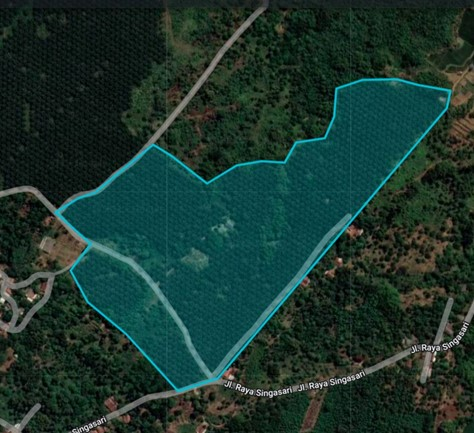
\includegraphics[width=1\columnwidth]{lampiran/Picture2.jpg}
	\end{center}
	\vspace{-0.2cm}
	%\rule{\columnwidth}{0.1pt}
	\captionsetup{justification=centering}
	%\caption{Gambar Hasil Citra Blok 1 untuk Uji Kebun Pendidikan dan Penelitian Kelapa Sawit IPB-Cargil}
	Gambar Hasil Citra Blok 1 untuk Uji Kebun Pendidikan dan Penelitian Kelapa Sawit IPB-Cargil
	%\label{img:Lampiran2}
\end{figure}
%%%%%%%%%%%%%%%%%%%%%%%%%% GAMBAR %%%%%%%%%%%%%%%%%%%%%%%%%%%%%%

%%%%%%%%%%%%%%%%%%%%%%%%%% GAMBAR %%%%%%%%%%%%%%%%%%%%%%%%%%%%%%
\begin{figure}[H]
	\vspace{-0.1cm}
	%\rule{\columnwidth}{0.1pt}
	\begin{center}
		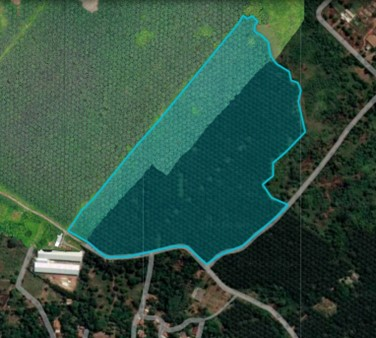
\includegraphics[width=0.7\columnwidth]{lampiran/Picture3.jpg}
	\end{center}
	\vspace{-0.2cm}
	%\rule{\columnwidth}{0.1pt}
	\captionsetup{justification=centering}
	%\caption{Gambar Hasil Citra Blok 1 untuk Uji Kebun Pendidikan dan Penelitian Kelapa Sawit IPB-Cargil}
	Gambar Hasil Citra Blok 2 untuk Uji Kebun Pendidikan dan Penelitian Kelapa Sawit IPB-Cargil
	%\label{img:Lampiran2}
\end{figure}
%%%%%%%%%%%%%%%%%%%%%%%%%% GAMBAR %%%%%%%%%%%%%%%%%%%%%%%%%%%%%%

%%%%%%%%%%%%%%%%%%%%%%%%%% GAMBAR %%%%%%%%%%%%%%%%%%%%%%%%%%%%%%
\begin{figure}[H]
	\vspace{-0.1cm}
	%\rule{\columnwidth}{0.1pt}
	\begin{center}
		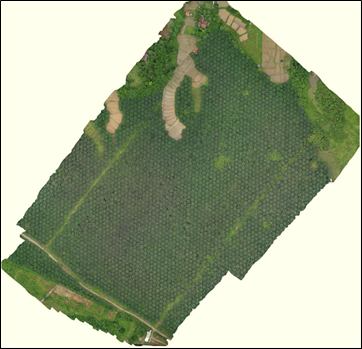
\includegraphics[width=0.7\columnwidth]{lampiran/Picture4.png}
	\end{center}
	\vspace{-0.2cm}
	%\rule{\columnwidth}{0.1pt}
	\captionsetup{justification=centering}
	%\caption{Gambar Hasil Citra Blok 1 untuk Uji Kebun Pendidikan dan Penelitian Kelapa Sawit IPB-Cargil}
	Gambar Hasil Citra Blok 3 untuk Dataset Primer Kebun Pendidikan dan Penelitian Kelapa Sawit IPB-Cargil
	%\label{img:Lampiran2}
\end{figure}
%%%%%%%%%%%%%%%%%%%%%%%%%% GAMBAR %%%%%%%%%%%%%%%%%%%%%%%%%%%%%%

%%%%%%%%%%%%%%%%%%%%%%%%%% GAMBAR %%%%%%%%%%%%%%%%%%%%%%%%%%%%%%
\begin{figure}[H]
	\vspace{-0.1cm}
	%\rule{\columnwidth}{0.1pt}
	\begin{center}
		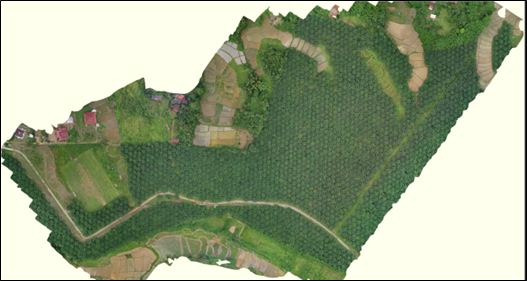
\includegraphics[width=0.9\columnwidth]{lampiran/Picture5.png}
	\end{center}
	\vspace{-0.2cm}
	%\rule{\columnwidth}{0.1pt}
	\captionsetup{justification=centering}
	%\caption{Gambar Hasil Citra Blok 1 untuk Uji Kebun Pendidikan dan Penelitian Kelapa Sawit IPB-Cargil}
	Gambar Hasil Citra Blok 4 untuk Dataset Primer Kebun Pendidikan dan Penelitian Kelapa Sawit IPB-Cargil
	%\label{img:Lampiran2}
\end{figure}
%%%%%%%%%%%%%%%%%%%%%%%%%% GAMBAR %%%%%%%%%%%%%%%%%%%%%%%%%%%%%%

%%%%%%%%%%%%%%%%%%%%%%%%%% GAMBAR %%%%%%%%%%%%%%%%%%%%%%%%%%%%%%
\begin{figure}[H]
	\vspace{-0.1cm}
	%\rule{\columnwidth}{0.1pt}
	\begin{center}
		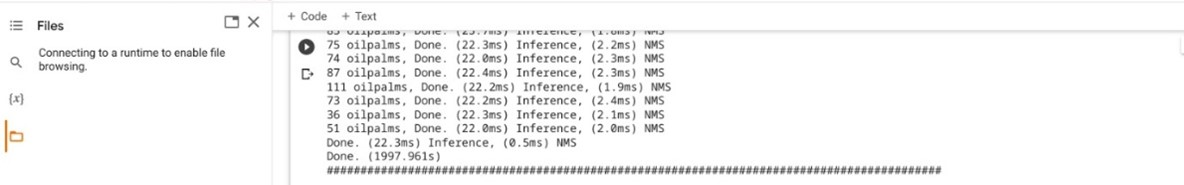
\includegraphics[width=0.9\columnwidth]{lampiran/Picture6.jpg}
	\end{center}
	\begin{center}
		
\includegraphics[width=0.9\columnwidth]{lampiran/Picture7.jpg}
	\end{center}
	\vspace{-0.2cm}
	%\rule{\columnwidth}{0.1pt}
	\captionsetup{justification=centering}
	%\caption{Gambar Hasil Citra Blok 1 untuk Uji Kebun Pendidikan dan Penelitian Kelapa Sawit IPB-Cargil}
	Gambar Hasil Uji Kecepatan Inferensi Model YOLOv7
	%\label{img:Lampiran2}
\end{figure}
%%%%%%%%%%%%%%%%%%%%%%%%%% GAMBAR %%%%%%%%%%%%%%%%%%%%%%%%%%%%%%
	% #akhir membuat daftar isi, daftar gambar dan  daftar tabel # =======================
	
	
	
	% # mulai bagian isi # =================================================================
	\newpage
	\pagestyle{headings}
	\doublespacing
	\pagenumbering{arabic} % jenis huruf arabic
	\setcounter{page}{1} %mulai dari halaman 1
	\pagestyle{fancy}
	\fancyhead[LO,RE]{\slshape \leftmark}
	\rhead{\thepage}
	\cfoot{}
	
	\chapter{PENDAHULUAN}
\titlespacing*{\chapter}{0pt}{0pt}{0pt}
\section{Latar Belakang}
\label{sec:1-LatarBelakang}

\hspace{1,2cm}Perkembangan teknologi yang pesat telah membantu dalam menjalani kehidupan yang lebih sederhana dan praktis. Permintaan untuk pengembangan teknologi terus meningkat dan telah menjadi salah satu bidang pekerjaan dan studi yang paling popular\citep{UnderstandingTheRoleOfDigital2022}. Perkembangan teknologi, khususnya investasi teknologi informasi dikaitkan dengan pertumbuhan produktivitas yang signifikan di negara maju dan berkembang \citep{InformationTechnologyAndProductivity2014}. Di negara-negara berkembang, teknologi informasi dan komunikasi sangat membutuhkan penerapan khsusunya di bidang pertanian. Pertanian memainkan peran sentral dalam pembangunan di banyak negara. Akses pasar, pembiayaan, dan pengetahuan adalah landasan pertumbuhan pertanian. Teknologi Informasi dan Komunikasi (TIK) mendukung petani dengan harga pasar secara real-time, prakiraan cuaca, hama, varietas benih dan teknik penanaman, identifikasi dan penghitungan tanaman. Pertanian juga merupakan sumber pendapatan utama bagi penduduk pedesaan di sebagian besar negara. Sektor ini menghadapi banyak tantangan untuk meningkatkan produksi. TIK memiliki potensi untuk memenuhi tantangan yang dihadapi oleh petani dan atau pemangku kepentingan yang dapat meningkatkan taraf hidup masyarakat pedesaan\citep{TheRoleandPotential2020}.

Dalam kasus ini, Indonesia adalah salah satu produsen dan eksportir pertanian terbesar di dunia, yang memasok bahan mentah penting seperti karet alam, kopi, kakao, beras, dan minyak kelapa sawit ke seluruh dunia. Dalam beberapa dekade terakhir, industri pertanian juga telah menjadi sektor yang paling banyak menyerap tenaga kerja di Indonesia (Statista Research, 2023). Indonesia juga sebagai produsen perkebunan terbesar di dunia, seperti karet alam dan kelapa sawit, produksi tanaman Indonesia sangat penting bagi perekonomian nasional. Dari 15 produk pertanian utama Indonesia, kelapa sawit merupakan yang terbesar. Produksi kelapa sawit sangat penting bagi perekonomian, karena Indonesia produsen dan konsumen terbesar di dunia dan menyumbang sekitar setengah dari pasokan dunia. Sebagian minyak kelapa sawit berasal dari perkebunan yang dikelola oleh petani kecil dengan luas 6,02 juta hektar pada tahun 2021. Petani kecil menghasilkan sekitar 34,36\% produksi minyak kelapa sawit, menjadikan petani kecil sebagai kontributor penting dalam mempromosikan industri kelapa sawit yang berkelanjutan di Indonesia \citep{DItjenbun-2022-Statistik-Perkebunan-Unggulan}.

Dalam menghasilkan produksi kelapa sawit yang baik, maka dibutuhkan penerapan teknologi yang mendukung untuk dapat memonitoring pohon kelapa sawit tersebut yang dapat menghasilkan, karena luas lahan yang begitu besar tidak memungkinkan dapat dikerjakan secara konvensional.

Pertanian presisi membutuhkan informasi yang dapat diandalkan tentang situasi terkini pada waktu yang tepat. Manajer kelapa sawit biasanya mengukur kepadatan atau jumlah pohon kelapa sawit secara manual. Tanaman kelapa sawit juga memiliki lahan yang luas, maka diperlukan pemantauan lahan secara berkala untuk mengontrol produktivitas kelapa sawit dan juga sebagai data inventaris, oleh karena itu, identifikasi otomatis dan lokasi kelapa sawit merupakan cara alternatif bagi petani untuk mengelola sumber daya mereka dengan menggunakan teknologi, bukan dengan pendekatan manual.

Kelapa sawit yang memiliki nama ilmiah (\textit{Elaeis guineensis Jacq.}) merupakan tanaman yang berasal dari daerah Benua Afrika dan negara di Amerika Selatan. Pada awalnya tanaman ini tumbuh liar dan setengah liar di daerah tepi sungai. Di Indonesia, tanaman ini pertama kali diperkenalkan oleh pemerintah colonial Belanda pada tahun 1848 di Kebun Raya Bogor \citep{IPahan2018}. Perkebunan kelapa sawit di Indonesia berkembang pesat, pada tahun 1939, Indonesia menjadi negara produsen dan eksportir utama kelapa sawit dunia dengan volume mencapai 244 ribu ton atau sebesar 48\% total ekspor minyak kelapa sawit dunia \citep{prayitno2008produktivitas}.

Besar volume dari kelapa sawit yang diproduksi oleh Indonesia menjadikan sector kelapa sawit membantu ekonomi Indonesia. Dalam perekonomian makro ekonomi Indonesia, industri atau sector kelapa sawit telah memiliki peran strategis, diantaranya penghasil devisa terbesar, lokomotif perekonomian nasional, kedaulatan energy, pendokorong sector ekonomi kerakyatan, dan penyerapan tenaga kerja. Hal ini dilihat dari besarnya perkebunan sawit di Indonesia. Perkebunan kelapa sawit Indonesia berkembang di 22 provinsi dari 33 provinsi. Dua pulau utama sentra perkebunan kelapa sawit yaitu Sumatera dan Kalimantan. Sekitar 90\% perkebunan kelapa sawit di Indonesia berada pada dua pulau tersebut, dan kedua pulau tersebut telah menghasilkan 95\% produksi minyak sawit mentah (\textit{crude palm oil/CPO}) Indonesia. Dalam perjalananya perkebunan kelapa sawit mengalami revolusi dan berkembang dengan cepat. Dalam kurun 1990-2015, tumbuh dan berkembangnya perkebunan rakyat dengan cepat, yakni, 24\% per tahun selama periode 1990-2015. Pada tahun 2015, luas perkebunan sawit di Indonesia adalah 11,3 juta hektar (KPRI, 2015)\citep{StatistikPerkebunanKelapaSawit2013-2015}. Menurut Ketua Asosiasi Industri Minyak Makan Indonesia (AIMMI) Adi Wisoko Kasman menjelaskan bahwa peningkakan konsumsi minyak kelawa sawit dalam negeri terus mengalami peningkatan \citep{GapkiCatatKonsumsiMinyakSawit}. Pada tahun 2019, konsumsi minyak sawit tumbuh hingga 23,57\% atau meningkat dari 13,49 juta ton di 2018 menjadi 16,67 juta ton di tahun 2019, kemudian konsumsi minyak sawit untuk kategori makanan (food) dalam negeri mencapai 9,86 juta ton atau naik hingga 49\% tahun per tahun \citep{EksporMinyakSawitKontanCoId}. Pada tahun 2021, hasil reevaluasi luas areal dari direktorat jenderal perkebunan, diketahui bahwa perkebunan besar swasta sebesar 60,64\%, diikuti perkebunan rakyat 34,36\%, dan perkebunan negara 5\% dari 14.621.690 ha. Pada tahun 2023, CPO Indonesia diprediksi mencapai 48,2 juta ton \citep{DItjenbun-2022-Statistik-Perkebunan-Unggulan}. Luas areal dan produksi kelapa sawit menurut provinsi dan status pengusahaan tahun 2021, seperti Tabel \ref{tabel-Statistik-Areal-Produksi-Kelapa-Sawit} berikut ini:

%%%%%%%%%%%%%%%%%%%%%%%%%% TABEL %%%%%%%%%%%%%%%%%%%%%%%%%%%%%%
\begin{table}[h]
\centering
\caption{Statistik Areal dan Produksi Kelapa Sawit Menurut Provinsi dan Status Pengusahaan Tahun 2021\\(Sumber: Ditjenbun, 2023)}
\label{tabel-Statistik-Areal-Produksi-Kelapa-Sawit}
	\begin{adjustbox}{width=\columnwidth,center}
	\begin{tabular}{|cc|cc|cc|cc|}
		\hline
		\multicolumn{2}{|c|}{\begin{tabular}[c]{@{}c@{}}Perkebunan Rakyat \\ Smallholders\end{tabular}}                                                             & \multicolumn{2}{c|}{\begin{tabular}[c]{@{}c@{}}Perkebunan Negara\\ Government Estate\end{tabular}}                                                         & \multicolumn{2}{c|}{\begin{tabular}[c]{@{}c@{}}Perkebunan Swasta\\ Private Estate\end{tabular}}                                                            & \multicolumn{2}{c|}{\begin{tabular}[c]{@{}c@{}}Jumlah \\ (Total)\end{tabular}}                                                                             \\ \hline
		\multicolumn{1}{|c|}{\begin{tabular}[c]{@{}c@{}}Luas/\\ Areal\\ (Ha)\end{tabular}} & \begin{tabular}[c]{@{}c@{}}Produksi/\\ Production\\ (Ton)\end{tabular} & \multicolumn{1}{c|}{\begin{tabular}[c]{@{}c@{}}Luas/\\ Areal\\ (Ha)\end{tabular}} & \begin{tabular}[c]{@{}c@{}}Produksi/\\ Production\\ (Ton)\end{tabular} & \multicolumn{1}{c|}{\begin{tabular}[c]{@{}c@{}}Luas/\\ Areal\\ (Ha)\end{tabular}} & \begin{tabular}[c]{@{}c@{}}Produksi/\\ Production\\ (Ton)\end{tabular} & \multicolumn{1}{c|}{\begin{tabular}[c]{@{}c@{}}Luas/\\ Areal\\ (Ha)\end{tabular}} & \begin{tabular}[c]{@{}c@{}}Produksi/\\ Production\\ (Ton)\end{tabular} \\ \hline
		\multicolumn{1}{|c|}{6.029.749}                                                    & 15.503.840                                                             & \multicolumn{1}{c|}{550.333}                                                      & 2.256.134                                                              & \multicolumn{1}{c|}{8.041.068}                                                    & 27.361.506                                                             & \multicolumn{1}{c|}{14.621.690}                                                   & 45.121.480                                                             \\ \hline
	\end{tabular}
	\end{adjustbox}
\end{table}
%%%%%%%%%%%%%%%%%%%%%%%%%% TABEL %%%%%%%%%%%%%%%%%%%%%%%%%%%%%%

Berdasarkan Tabel \ref{tabel-Statistik-Areal-Produksi-Kelapa-Sawit} bahwa saat ini areal dan produksi kelapa sawit masih dikuasai dan dikelola oleh Perkebunan Swasta yang tersebar dari 34 provinsi di Indonesia, yaitu luas areal sebesar 8.041.068 (Ha) dan dapat memproduksi 27.361.506 (Ton) dari 45.121.480 (Ton) (Ditjebun, 2023).

Dari data yang diperoleh menurut Ditjenbun tahun 2023 bahwa dibutuhkan kelapa sawit dalam jumlah yang besar dan produksi minyak sawit yang dihasilkan dari kelapa sawit tersebut harus baik. Pohon kelapa sawit membutuhkan waktu sekitar 4 (empat) tahun untuk menghasilkan buah yang sesuai untuk panen. Setiap pohon kelapa sawit kemudian akan terus menghasilkan buah hingga usia 25 tahun. Menurut Smart Agribusiness and food dalam artikelnya menyebutkan bahwa pohon kelapa sawit ini memanfaatkan teknologi pertanian didukung oleh analisis satelit di seluruh area perkebunan, sehingga pemanfaatan hasil panen dapat dihasilkan hasil panen dapat digunakan secara optimal (Smart Agribusiness and Food, 2017). Dalam pengelolaan perkebunan kelapa sawit, populasi dalam satuan hektar (ha) sangat penting dan hal ini berhubungan dengan pengaruh jarak tanam. Jarak tanam merupakan faktor yang mempengaruhi pertumbuhan tanaman kelapa sawit. Pengaturan jarak tanam bertujuan untuk mendapatkan ruang tumbuh bagi pertumbuhan tanaman guna menghindari kompetisi unsur hara dan cahaya matahari dari setiap tanaman kelapa sawit pada jarak tanam yang berbeda. Jarak tanam 9x9x9 m baik untuk kelapa sawit (Hayata et al, 2020). Kepadatan pada jarak tanam normal biasanya bervariasi sesuai dengan jenis tanah yang ditanami kelapa sawit. Jumlah tanaman kelapa sawit pada pesisir dan di tanah mineral adalah antara 136 - 148 kelapa sawit/hektar seperti pada Gambar \ref{img:bab1-area-lahan-IPB}, sedangkan di tanah gambut, jarak tanamnya biasanya lebih padat, sekitar 150 kelapa sawit/hektar (J. Latif et al., 2003). Gambar \ref{img:bab1-area-lahan-IPB} merupakan area lahan Kebun Pendidikan dan Penelitian IPB Cargil - Jonggol Blok 3 dengan tanah mineral (J. Albari et al., 2018). Tanah mineral adalah tanah yang terbentuk dan berkembang dari bahan mineral, melalui proses pelapukan, baik secara fisis maupun kimia, didominasi oleh pelapukan bebatuan \citep{Mineral-Water-Sebagai-Indikator}.

%%%%%%%%%%%%%%%%%%%%%%%%%% GAMBAR %%%%%%%%%%%%%%%%%%%%%%%%%%%%%%
\begin{figure}[H]
	\vspace{-0.1cm}
	%\rule{\columnwidth}{0.1pt}
	\begin{center}
		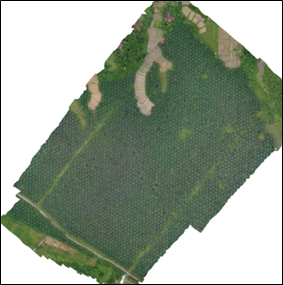
\includegraphics[width=0.5\columnwidth]{bab1/Gambar/Picture1.png}
	\end{center}
	\vspace{-0.2cm}
	%\rule{\columnwidth}{0.1pt}
	\caption{Area Lahan Kelapa Sawit IPB Cargil Jonggol Blok 3 Jarak Tanam 9x9x9}\label{img:bab1-area-lahan-IPB}
\end{figure}
%%%%%%%%%%%%%%%%%%%%%%%%%% GAMBAR %%%%%%%%%%%%%%%%%%%%%%%%%%%%%%

Dalam memenuhi kebutuhan minyak kelapa sawit, selain membutuhkan areal lahan, dibutuhkan pola tanam dan jarak tanam kelapa sawit yang tepat. Pola tanam kelapa sawit yang baik dibutuhkan perhatikan yang lebih karena berkaitan dengan efektifitas penggunaan lahan. Pola tanam segitiga sama sisi merupakan pola tanam yang paling efektif di areal datar, sehingga untuk areal bergelombang atau berbukit perlu dilakukan "viol linning" untuk mempertahankan jumlah populasi per hektarnya dengan tetap memperhatikan tingkat kesuburan tanahnya (GD Morganic, 2018), ilustrasi jarak tanam kelapa sawit seperti pada Gambar \ref{img:bab1-Pola-Tanam-dan-Jarak-Tanam}.

%%%%%%%%%%%%%%%%%%%%%%%%%% GAMBAR %%%%%%%%%%%%%%%%%%%%%%%%%%%%%%
\begin{figure}[H]
	\vspace{-0.1cm}
	%\rule{\columnwidth}{0.1pt}
	\begin{center}
		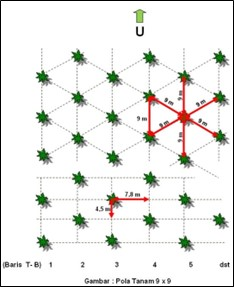
\includegraphics[width=0.5\columnwidth]{bab1/Gambar/Picture2.jpg}
	\end{center}
	\vspace{-0.2cm}
	%\rule{\columnwidth}{0.1pt}
	\caption{Pola Tanam dan Jarak Tanam Kelapa Sawit yang Tepat\\(Sumber: GD Morganic, 2018)}\label{img:bab1-Pola-Tanam-dan-Jarak-Tanam}
\end{figure}
%%%%%%%%%%%%%%%%%%%%%%%%%% GAMBAR %%%%%%%%%%%%%%%%%%%%%%%%%%%%%%

Direktorat Jenderal Perkebunan (Ditjenbun) memetakan memetakan produksi kelapa sawit menurut provinsi dan menunjukkan bahwa provinsi Riau memiliki produksi terbesar 2021 sebesar 8,96 juta ton dengan luas 3,49 juta hektar (Ditjenbun, 2023). Berikut ini Gambar \ref{img:bab1-Peta-10-Besar-Provinsi}. peta kelapa sawit Indonesia berdasarkan Direktorat Jenderal Perkebunan.

%%%%%%%%%%%%%%%%%%%%%%%%%% GAMBAR %%%%%%%%%%%%%%%%%%%%%%%%%%%%%%
\begin{figure}[H]
	\vspace{-0.1cm}
	%\rule{\columnwidth}{0.1pt}
	\begin{center}
		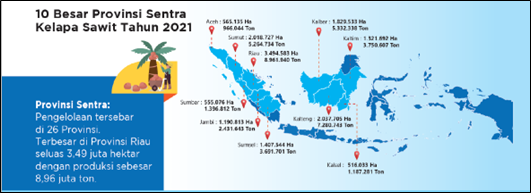
\includegraphics[width=1\columnwidth]{bab1/Gambar/Picture3.png}
	\end{center}
	\vspace{-0.2cm}
	%\rule{\columnwidth}{0.1pt}
	\caption{Peta 10 Besar Provinsi Sentra Kelapa Sawit Tahun 2021\\(Sumber: Ditjenbun, 2023)}\label{img:bab1-Peta-10-Besar-Provinsi}
\end{figure}
%%%%%%%%%%%%%%%%%%%%%%%%%% GAMBAR %%%%%%%%%%%%%%%%%%%%%%%%%%%%%%

Direktorat jenderal perkebunan juga mencatat estimasi luas area dan produksi minyak sawit Indonesia tahun 2023 mencapai 48,24 juta ton dan luas hektar mencapai 15,3 juta ton (Ditjenbun, 2023) seperti pada Gambar  \ref{img:bab1-Estimasi-Luas-Area-Produksi-Minyak}.

%%%%%%%%%%%%%%%%%%%%%%%%%% GAMBAR %%%%%%%%%%%%%%%%%%%%%%%%%%%%%%
\begin{figure}[H]
	\vspace{-0.1cm}
	%\rule{\columnwidth}{0.1pt}
	\begin{center}
		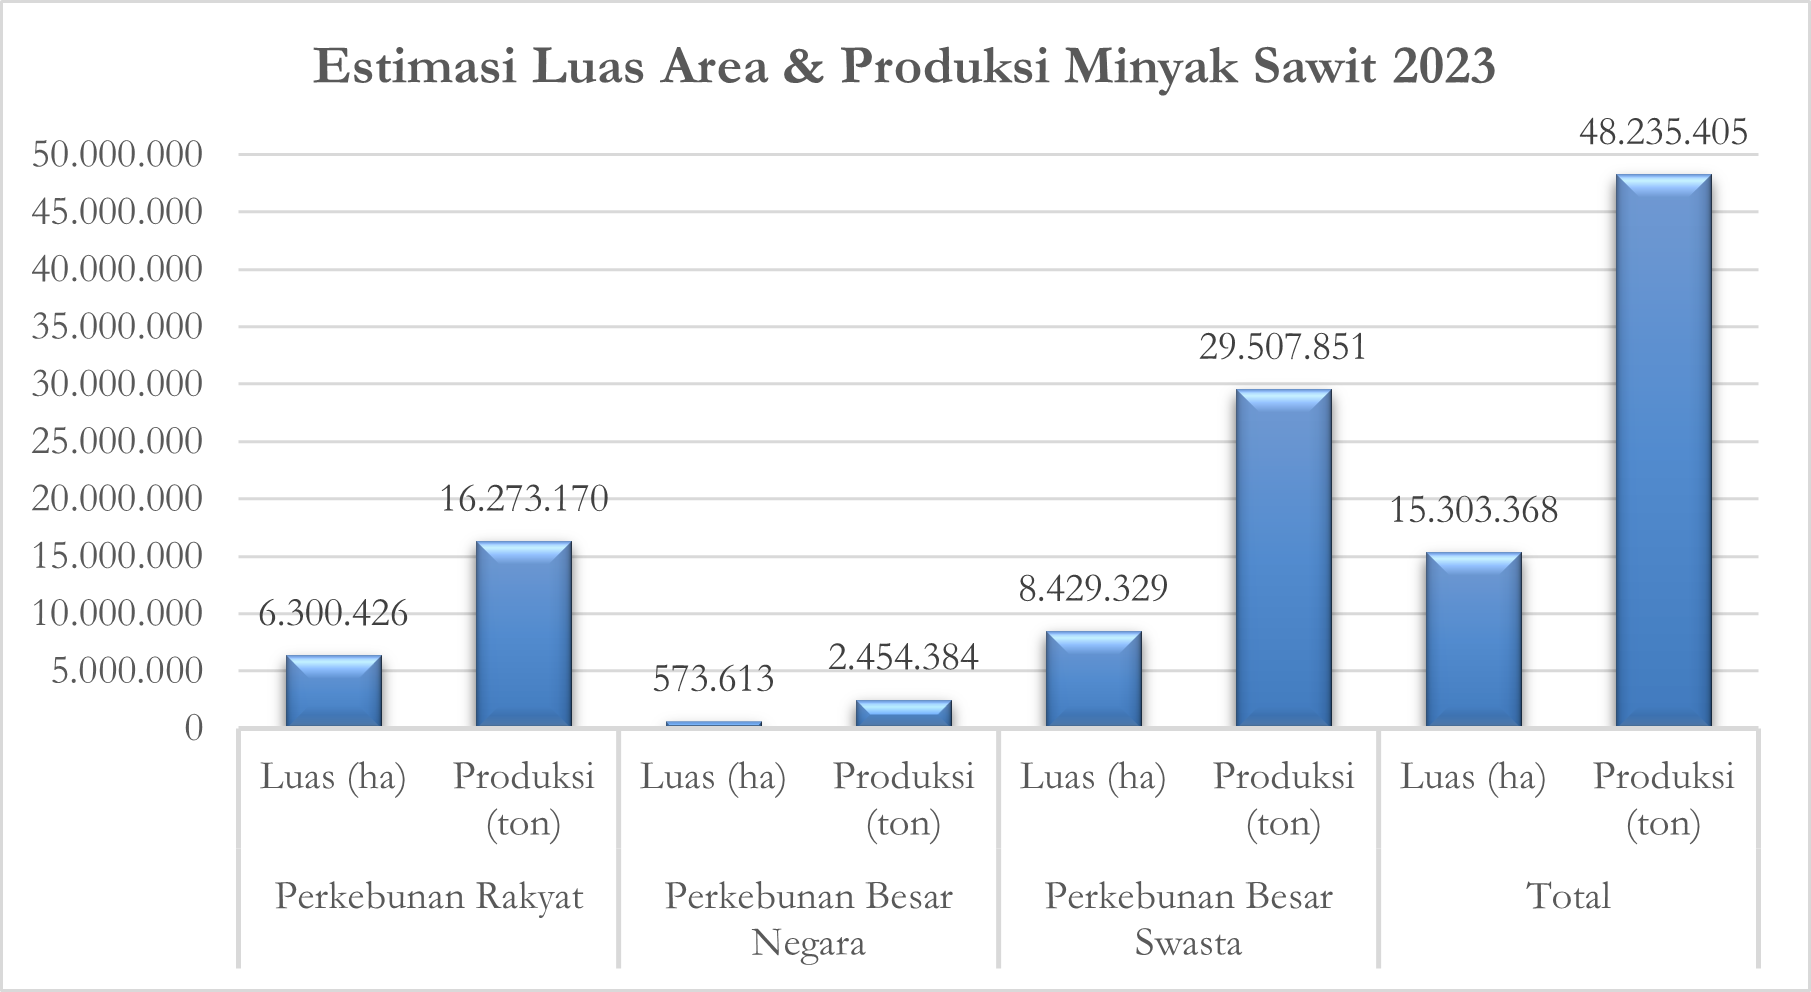
\includegraphics[width=1\columnwidth]{bab1/Gambar/Picture4.png}
	\end{center}
	\vspace{-0.2cm}
	%\rule{\columnwidth}{0.1pt}
	\caption{Estimasi Luas Area dan Produksi Minyak Sawit Indonesia 2023\\Sumber: (Ditjenbun, 2023)}\label{img:bab1-Estimasi-Luas-Area-Produksi-Minyak}
\end{figure}
%%%%%%%%%%%%%%%%%%%%%%%%%% GAMBAR %%%%%%%%%%%%%%%%%%%%%%%%%%%%%%

Gambar \ref{img:bab1-Estimasi-Luas-Area-Produksi-Minyak} menyatakan bahwa perkebunan swasta (PBS) menguasasi sebanyak 61,2\% dengan total produksi 29,5 juta ton, perkebunan rakyat (PR) sebesar 33,7\% dengan total produksi sebanyak 16,2 juta ton, sedangkan perkebunan besar negara (PBN) hanya 5\% dengan total 2,45 juta ton. 

Jumlah estimasi luas area lahan pohon kelapa sawit yang besar juga menjadikan permasalahan bagi pengelolaan perkebunan kelapa sawit. Dari sisi agronomis, bahwa batasan minimum untuk perusahaan perkebunan kelapa sawit yaitu sebesar 6.000 (enam ribu) hektar yang harus dikelola (PPRI, 2021). Luas lahan untuk petani kelapa sawit yang didefinisikan sebagai petani kelapa sawit adalah tingal di pedesaan/sekitar kebun yang dimana kelapa sawit sebagai mat apencaharian utama, dikerjakan dan dikontrol sendiri oleh keluarganya, dan mengalami kesulitan karena bibit yang digunakan disemai sendiri dan tidak bersertifikat, sulit mengakses area karena luas, serta produktivitas rendah menjadi permasalahan utama (SPKS, 2020). Di samping permasalahan luas area ini, lokasi perkebunan sawit juga berada pada remote area, yaitu area atau daerah yang terpencil, jauh dari peradaban (daerah pedalaman atau pelosok hutan) yang dimana karena lokasi perkebunan kelapa sawit yang luas, sehingga sulit dimonitoring tanpa teknologi informasi. Permasalahan yang ada bahwa di perkebunan kelapa sawit yang luas juga terkendala akses infrastruktur, seperti jalan yang belum memadai untuk akses kendaraan, seperti di Kebun Pendidikan dan Penelitian IPB-Cargil akses jalan bergelombang dan masih bebatuan, dan menurut dinas perkebunan provinsi Kalimantan timur bahwa infrastruktur dan aksesibilitas terhubung dengan baik, maka produktivitas dan kegiatan monitoring kawasan perkebunan kelapa sawit akan sangat membantu (Disbun, 2014). Produksi per individu tanaman pohon kelapa sawit berkontribusi besar terhadap produktivitas karena setiap pohon kelapa sawit akan menghasilkan buah kelapa sawit yang dapat diproduksi dan dipanen hasilnya untuk masyarakat, sehingga data pohon kelapa sawit sangat penting untuk dilakukan. Selain itu, salah satu upaya yang dilakukan dalam perkebunan kelapa sawit adalah masalah pemupukan. Adanya peningkatan produksi melalui intensifikasi dengan pemberian pupuk yang presisi, secara cepat, dan akurat, serta up-to-date pada suatu luasan lahan.  Upaya yang dapat dilakukan adalah dengan meningkatkan produktivitas melalui peningkatan efektivitas dan efisiensi penggunaan pupuk. Efektivitas dan efisiensi pemberian pupuk sangat penting dilakukan karena biaya pemupukan tanaman kelapa sawit sangat besar yaitu 50\%-70\% dari biaya pemeliharaan dan 25\% dari seluruh biaya produksi (Fairhurst et al., 2006). Penambahan unsur hara dapat meningkatkan pertumbuhan tanaman, produksi tanaman, dan kualitas produk yang dihasilkan, seperti buah kelapa sawit (S. Parman, 2007).	

Buah kelapa sawit yang dapat dihasilkan di Indonesia cukup besar dan harus diproduksi atau dipanen dengan baik, agar hasil dari buah kelapa sawit yang mayoritas menjadi minyak menghasilkan minyak yang berkualitas. Hal ini berkenaan dengan standar mutu kematangan buah kelapa sawit yang dikenal dengan standar kematangan panen. Buah sawit bergerombol dalam tandan yang muncul dari tiap pelapah. Minyak dihasilkan oleh buah. Kandungan minyak bertambah sesuai dengan tingkat kematangan buah. Penghitungan pohon kelapa sawit yang menghasilkan minyak dapat dilakukan secara manual di lapangan, tetapi ini menghabiskan waktu, membutuhkan pekerja yang tidak sedikit, dan mahal\citep{Mubin2019-xq}. Disamping itu, Manajer perkebunan kelapa sawit biasanya mengukur kepadatan kelapa sawit secara manual setiap tahun. Data penting ini dapat digunakan untuk memperkirakan produktivitas kelapa sawit, jumlah pupuk yang dibutuhkan, biaya penyiangan berkala, dan jumlah pekerja yang dibutuhkan, dan terkait dengan kegiatan lain (J. W. Kiama, 2014).

Oleh karena itu, dibutuhkan suatu metode atau teknologi untuk membantu mengklasifikasikan atau mendeteksi jumlah dan estimasi usia pohon kelapa sawit untuk dapat diketahui tingkat kematangan buah kelapa sawit, maka dapat diproduksi (dipanen) dengan baik, sehingga produksi yang dihasilkan dapat mencapai optimum. Berikut ini penelitian-penelitian yang telah dilakukan penelitian sebelumnya.

Klasifikasi berbasis piksel sering digunakan untuk mengklasifikasikan kelas fitur dari gambar. Metode Object-Based Image Analysis (OBIA) telah berevolusi untuk menganalisis gambar resolusi tinggi dengan cepat (T. Blaschke, 2010), dengan semakin tersedianya resolusi tinggi dan citra skala besar, maka dihasilkan cara baru untuk memulai penelitian tentang interpretasi foto pohon berbasis komputer (P. Gong et al, 1999). OBIA dikembangkan oleh Hay dan Castilla merupakan disiplin ilmu spasial yang berfokus pada pengelompokkan citra penginderaan jauh ke makna objek penuh melalui pemanfaatan spasial \citep{Hay2008-vt}. Gagasan menganalisis gambar dalam ruang objek daripada ruang pixel dikembangkan karena kekurangan metode berbasis pixel, terutama pada gambar resolusi tinggi. Selain itu, ruang objek telah diperkuat dalam kapasitas komputasi dan ketersediaan untuk analisis gambar resolusi tinggi seperti IKONOS, GeoEye, dan WorldView (T. Blaschke, 2010).

Jusoff dan Pathan menggunakan airborne hyperspectral sensing linear analis campuran spectral, bersama dengan campuran ke konventer murni dan norma Euclidean teknik untuk memetakan masing-masing pohon kelapa sawit (K. Jusoff, 2009). Korom et all tahun 2014 mengelompokkan bentuk kanopi atau mahkota kelapa sawit menggunakan citra WorldView-2 berdasarkan segmentasi watershed dan mencapai akurasi sekitar 77\% \citep{Korom2014-ci}.

Wong-in et al. tahun 2015 telah mencapai akurasi 90\% menggunakan gambar udara dengan beberapa langkah, seperti menghapus komponen non-pohon dari gambar, membedakan munyak sawit dari komponen lain menggunakan filter low-pass dan korelasi silang dinormalisasi, mengidentifikasi pohon kelapa sawit secara individu dan menghitung jumlah pohon kelapa sawit \citep{Wong-in2015-jv}.

H. Santoso et al. pada tahun 2016 membangun dan mengembangkan metode yang mudah digunakan pengguna yang akan memungkinkan manajer kelapa sawit untuk menghitung minyak pohon kelapa sawit menggunakan teknik penginderaan jauh. Pohon kelapa sawit dianalisis dalam penilitian ini dengan melihat usia dan kepadatan yang berbeda. Penelitian ini menggunakan Citra QuickBird yang diaplikasikan dengan enam metode pansharpening. Hitam dan citra putih dari komposit warna palsu citra pansharpening diproses dalam tiga cara: (1) deteksi pohon kelapa sawit, (2) penggambaran area kelapa sawit, (3) penghitungan pohon kelapa sawit dan penilaian akurasi. Penelitian ini menggunakan ENVI 5.2, ERDAS Imagine 2015, dan ArcGIS 10.2.2. Hasil penelitian ini meningkat pada akurasi dari beberapa studi penelitian sebelumnya yang memiliki akurasi 90-95\%. Hasil dalam penelitian ini menunjukkan (1) gabungan resolusi intensitas huesaturation (HIS) cocok untuk kelapa sawit berusia 16 tahun, pohon dan memiliki kepadatan agak tinggi dengan akurasi 100\%, (2) untuk kelapa sawit berusia 21 tahun dan memiliki kepadatan rendah didapatkan hasil dengan akurasi 99,5\%, (3) resolusi subtraktif penggabungan ini cocok untuk pohon kelapa sawit berusia 15-18 tahun dan memiliki kerapatan yang agak tinggi dengan akurasi 99,8\%, (4) penajaman spectral PC dengan akurasi 99,3\% cocok untuk pohon kelapa sawit berusia 10 tahun dan memiliki kepadatan rendah, dan (5) untuk semua kondisi objek studi, warna dinormalisasi (Brovey) dan penggabungan resolusi wavelet adalah dua metode pansharpening yang cocok untuk ekstraksi dan kelapa sawit dengan penghitungan masing-masing dengan akurasi 98,9\% dan 98,4\% (H. Santoso et al, 2016).

H. M. Rizeei et al. tahun 2018 meneliti bahwa pemantauan karakteristik kelapa sawit di area perkebunan sangat berharga bagi petani dan stakeholders untuk memaksimalkan produktivitas. Penelitian ini mengusulkan metode baru untuk estimasi dan penghitungan usia kelapa sawit. Algoritma Support Vector Machine (SVM) dari analisis gambar berbasis objek (OBIA) diterapkan untuk penghitungan kelapa sawit. Analisis sensitivitas dilakukan pada empat jenis kernel SVM (Sigmoid (SIG), Linear (LN), fungsi basis radial (RBF), dan polynomial (PL)) dengan parameter terkait (Nilai ambang batas, Gamma ($\gamma$) dan faktor Penalti (c )) untuk mendapatkan pendekatan klasifikasi OBIA optimal untuk setiap blok perkebunan. Citra dengan resolusi sangat tinggi dari Worldview-3 (WV-3) digunakan untuk deteksi kelapa sawit. Hasil deteksi kelapa sawit memiliki akurasi keseluruhan 98,27\%, 99,48\%, 99,28\%, 99,49\%, dan 97,49\% untuk blok A, B, C, D, dan E \citep{Rizeei2018-yr}.

W Li et al tahun 2018 meneliti deteksi pohon kelapa sawit dalam skala besar dari gambar satelit beresolusi tinggi (QuickBird) menggunakan Two-Stage Convolutional \textit{Neural Networks} (TS-CNN). TS-CNN terdiri dari satu CNN untuk klasifikasi tutupan lahan dan satu CNN untuk klasifikasi objek. Kedua CNN dilatih dan dioptimalkan secara independen berdasarkan pada 20.000 sampel yang dikumpulkan melalui interpretasi manusia. Skala area pohon kelapa sawit sebesar 55 km2. Penelitian ini mengusulkan alur kerja yang efektif yang terdiri dari metode partisi yang tumpeng tindih untuk divisi gambar skala besar, metode \textit{multi-scale sliding window} untuk memprediksi koordinat kelapa sawit, dan metode filter jarak untuk pasca-pemrosesan. Pendekatan yang diusulkan mencapai skor F1 rata-rata yang jauh lebih tinggi yaitu 94,99\% di wilayah studi dibandingkan dengan metode deteksi kelapa sawit yang ada masing-masing sebesar (87,95\%, 81,80\%, 80,61\%, dan 78,35\% untuk CNN satu-tahap, \textit{Support Vector Machine} (SVM), \textit{Random Forest} (RF), dan \textit{Artificial Neural Network} (JST)), dan jauh lebih sedikit kebingungan dengan vegetasi dan bangunan lain di seluruh hasil deteksi gambar \citep{Li2018-eb}.

N. A. Mubin et al. tahun 2019 telah meneliti bahwa deteksi dan penghitungan kelapa sawit penting dalam pengelolaan perkebunan kelapa sawit. Dalam penelitian ini, digunakan pendekatan pembelajaran mendalam untuk memprediksi dan menghitung kelapa sawit dalam citra satelit. Deteksi kelapa sawit sebelumnya secara umum berfokus pada mendeteksi kelapa sawit yang tidak memiliki tumpeng tindih mahkota. Selain itu, terdapat kurangnya penelitian yang membangun sistem deteksi terpisah untuk kelapa sawit muda dan dewasa, memanfaatkan pendekatan pembelajaran mendalam untuk mendeteksi kelapa sawit dan menggabungan sistem informasi geografis (SIG) dengan pendekatan pembelajaran mendalam. Penelitian ini mencoba untuk mengisi kesenjangan ini dengan memanfaatkan dua jaringan saraf convolution (CNN) yang berbeda untuk mendeteksi kelapa sawit muda dan matang secara terpisah dan menggunakan GIS selama pemrosesan data dan proses penyimpanan hasil. Arsitektur awal yang dikembangkan didasarkan pada CNN yang disebut LeNet. Proses pelatihan mengurangi kerugian dengan menggunakan algoritma gradient adaptif dengan batch mini ukuran 20 untuk semua set pelatihan yang digunakan. Kemudian, mengekspor hasil prediksi ke perangkat lunak GIS dan membuat peta prediksi kelapa sawit dewasa dan muda. Berdasarkan metode yang diusulkan, akurasi keseluruhan untuk kelapa sawit muda dan matang masing-masing adalah 95,11\% dan 92,96\%. Secara keseluruhan, pengklasifikasi bekerja dengan baik pada dataset yang sebelumnya tidak terlihat, dan mampu secara akurat mendeteksi kelapa sawit dari latar belakang, termasuk bayangan tanaman lainnya (N. A. Mubin, 2019). 

\section{Batasan Penelitian}
\label{sec:2-BatasanMasalah}
\hspace{1,2cm}Ruang lingkup yang menjadi penelitian adalah:
\begin{enumerate}
	\item Dataset citra sebagai dataset primer berjumlah 69 citra dari Kebun Pendidikan dan Penelitian Kelapa Sawit IPB-Cargil, Jonggol, Jawa Barat dan 205 citra dari Universitas Gunadarma, PPU Campus, Kalimantan Timur yang ditanami pohon kelapa sawit.
	\item Dataset sekunder digunakan melalui akses roboflow secara free sebanyak 1795 citra dataset sekunder yang sudah memiliki label atau anotasi kelas 'oil palm'.
	\item Pengujian penerapan sistem menghitung dan mendeteksi pohon kelapa sawit dilakukan pada lahan pohon kelapa sawit tanah mineral Kebun Pendidikan dan Penelitian Kelapa Sawit IPB-Cargil, Jonggol Jawa Barat.
\end{enumerate}


\section{Rumusan Masalah}
\label{sec:3-Rumusanmasalah}
\hspace{1,2cm}Adapun rumusan masalah dalam penelitian ini secara umum bahwa pengelolaan perkebunan kelapa sawit memiliki permasalahan yang utama, diantaranya luas area pengelolaan kebun kelapa sawit dalam skala besar (perusahaan perkebunan kelapa sawit memiliki luas minimum sebesar 6.000 (enam ribu) hektar dan petani 4 hektar yang harus dikelola). Perkebunan berada di \textit{remote area}, area yang terpencil, daerah pedalaman atau pelosok hutan, yang sulit untuk dilakukan monitoring, dan akses infrastruktur terutama jalan yang terbatas dan sulit. Permasalahan yang dihadapi juga berupa pemupukan presisi yang mengalami kesulitan untuk mendapatkan secara akurat, dan cepat, serta \textit{up-to-date} jumlah tegakkan pohon kelapa sawit pada suatu luasan lahan tertentu, sementara praktik yang ada adalah menggunakan perhitungan manual dan normatif berbasis jarak tanam pohon kelapa sawit. Hal ini menyebabkan pentingnya data jumlah pohon kelapa sawit sangat penting dibutuhkan karena produksi per individu tanaman berkontribusi besar terhadap produktivitas dengan penyelesaian teknologi informasi. Berdasarkan permasalahan tersebut, maka rumusan masalah secara khusus:  
\begin{enumerate}
	\item Bagaimana membuat pengembangan metode \textit{object-based image analysis} (OBIA) untuk membuat dataset secara otomatis dengan memberikan anotasi atau label suatu kelas pada data citra?
	\item Bagaimana mendapatkan model CNN yang baik dari algoritma YOLOv5, YOLOv6, dan YOLOv7 untuk mendeteksi dan menghitung pohon kelapa sawit pada suatu area tertentu?
	\item Bagaimana mengembangkan sistem berbasis web dengan menerapkan model CNN dari algoritma YOLO agar dapat mendeteksi, menghitung, dan mendapatkan letak koordinat latitude-longitude setiap pohon kelapa sawit dari citra satelit agar dapat dilakukan pemantauan, pengelolaan, dan estimasi produktivitas secara otomatis?
\end{enumerate}

\section{Tujuan Penelitian}
\label{sec:4-BatasanMasalah}
\hspace{1,2cm}Adapun tujuan dari penelitian ini secara umum adalah menghasilkan purwarupa sistem berbasis web dengan menerapkan model OBIA dan \textit{Deep Learning} (DL) untuk mendeteksi, menghitung jumlah pohon dalam suatu luasan tertentu dan mendapatkan nilai koordinat latitude-longitude setiap pohon kelapa sawit dari citra satelit. Tujuan penelitian secara khusus sebagai berikut: 
\begin{enumerate}
	\item Menghasilkan metode object-based image analysis (OBIA) untuk membuat dataset secara otomatis dengan memberikan anotasi atau label suatu kelas, kelas 'oil palm' pada data citra.
	\item Menghasilkan model CNN dari algoritma YOLOv5, YOLOv6, dan YOLOv7 yang dapat mendeteksi dan menghitung pohon kelapa sawit pada suatu area tertentu.
	\item Menghasilkan purwarupa perangkat lunak aplikasi dengan model convolutional neural network dari algoritma YOLO yang terintegrasi dengan citra satelit dengan menggunakan Google Maps API yang dapat mendeteksi, menghitung, dan mendapatkan letak koordinat latitude-longitude setiap pohon kelapa sawit pada suatu area tertentu.
\end{enumerate}

\section{Kontribusi Hasil Penelitian}
\label{sec:5-Kontribusi-Hasil-Penelitian}
\hspace{1,2cm}Kontribusi penting dari penelitian yang dilakukan dalam penelitian ini adalah:
\begin{enumerate}
	\item Dari sisi keilmuan, berupa pengembangan metode \textit{object-based image analysis} (OBIA) untuk membuat dataset secara otomatis dengan memberikan anotasi atau label suatu kelas pada data citra dengan menggunakan algoritma \textit{template matching} dan BIRCH.
	\item Dari sisi teknologi, penelitian ini menghasilkan dataset primer dengan kelas pohon kelapa sawit (\textit{oil palm}) dan purwarupa perangkat lunak aplikasi dengan model \textit{convolutional neural network} dari algoritma YOLO yang terintegrasi dengan citra satelit dengan menggunakan Google Maps API yang dapat mendeteksi, menghitung, dan mendapatkan letak koordinat latitude-longitude setiap pohon kelapa sawit yang berhasil dideteksi.
	3.	Dari sisi pemanfaatan, menawarkan suatu cara alternatif untuk proses persiapan data citra untuk mendapatkan dataset dengan proses anotasi yang lebih cepat, serta bagi \textit{stakeholder} dapat memantau, mengelola, dan melakukan estimasi produktivitas secara otomatis pohon kelapa sawit pada suatu area tertentu dengan penerapan teknologi informasi.
	
\end{enumerate}

%%%%%%%%%%%%%%%%%%%%%%%%%%% GAMBAR %%%%%%%%%%%%%%%%%%%%%%%%%%%%%%
%\begin{figure}[!h]
%  \vspace{-0.1cm}
%%\rule{\columnwidth}{0.1pt}
%\begin{center}
%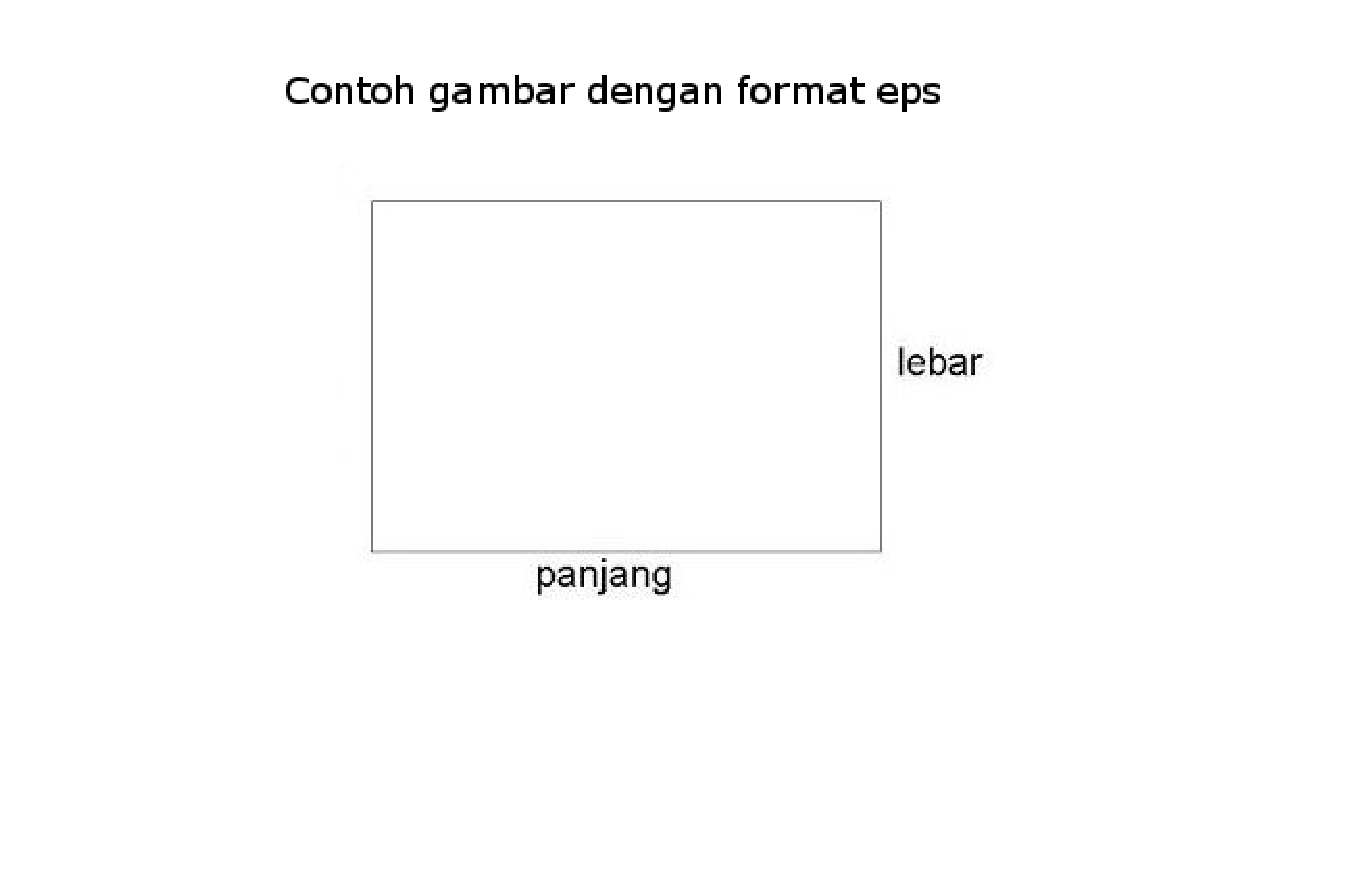
\includegraphics[width=0.8\columnwidth]{bab1/Gambar/gambar1-1.eps}
%\end{center}
%\vspace{-0.2cm}
%%\rule{\columnwidth}{0.1pt}
%\caption{Perbedaan Alur Desain FPGA dan Desain ASIC}\label{gambar1}
%\end{figure}
%%%%%%%%%%%%%%%%%%%%%%%%%%% GAMBAR %%%%%%%%%%%%%%%%%%%%%%%%%%%%%%

 %Bab 1
	\chapter{TELAAH PUSTAKA}
\label{cha:2-TelaahPustaka}

\vspace{1cm}
\section{\textit{Computer Vision}}
\hspace{1,2cm}\textit{Computer Vision} atau visi komputer adalah bidang kecerdasan buatan (AI) yang memungkinkan komputer dan sistem memperoleh informasi bermakna dari gambar digital, video, dan input visual lainnya, dan mengambil tindakan atau membuat rekomendasi berdasarkan informasi tersebut. Jika kecerdasan buatan memungkinkan komputer untuk berpikir, visi komputer memungkinkan untuk melihat, mengamati, dan memahami (IBM, 2020).

\textit{Computer vision} bekerja hamper sama dengan visi manusia, kecuali manusia memiliki permulaan. Penglihatan manusia memiliki keunggulan konteks seumur hidup untuk melatih cara membedakan objek, seberapa jauh jaraknya, apakah bergerak, dan apakah ada yang salah dalam sebuah gambar. \textit{Computer vision} melatih mesin untuk melakukan fungsi-fungsi melatih mesin untuk melakukan fungsi-fungsi ini, tetapi ia harus melakukannya dalam waktu yang jauh lebih singkat dengan kamera, data, dan algoritma daripada retina, saraf, optic, dan korteks visual karena sistem yang dilatih untuk memeriksa produk atau mengamati asset produksi dapat menganalisis ribuan produk atau proses dalam satu menit, memperhatikan cacat atau masalah yang tidak terlihat, sistem tersebut dapat dengan cepat melampaui kemampuan manusia. 

Memahami dan menentukan tugas visi komputer tertentu dapat memfokuskan dan memvalidasi proyek dan aplikasi, serta mempermudah untuk memulai. Hal dasar untuk \textit{computer vision} adalah \textit{object detection}, beberapa tugas visi komputer lainnya, seperti \textit{image classification, object detection, object tracking}, dan \textit{content-based image retrieval} (U. Arshad, 2021).

\vspace{1cm}
\section{Pengertian Citra}
Citra didefinisikan sebagai fungsi dari dua variabel misalnya \textit{a(x,y)} dimana a sendiri sebagai amplitudo (misalnya kecerahan) citra pada koordinat (x,y) (I. T. Young et al, 1995). Citra digital a[m,n] merupakan citra dalam ruang diskrit 2D yang berasal dari citra analog a(x,y) di ruang kontinyu 2D melalui proses sampling yaitu yang biasa disebut sebagai digitalisasi. Sedangkan, menurut Maria citra digital adalah citra f(x,y) yang telah didiskritkan oleh pada koordinat spasial dan kecerahan. Citra digital direpresentasikan oleh \textit{array} dua dimensi atau sekumpulan \textit{array} dua dimensi dimana setiap \textit{array} merepresentasikan satu kanal warna. Nilai kecerahan yang didigitalkan dinamakan nilai tingkat keabuan (A. McAndrew, 2004).

Setiap elemen \textit{array} tersebut dinamakan piksel yang diambil dari istilah \textit{picture element}. Dimensi citra biasanya ditulis dengan format panjang x tinggi (misalnya 640 x 480 piksel). Namun, perlu diperhatikan dengan seksama bahwa secara matematis, definisi citra terlihat seperti di bawah ini, dimana x menunjukkan baris dan y menunjukkan kolom:

\[
f(x,y)=
\begin{bmatrix}
	f\left(0,0\right)  & f\left(0,1\right) & ... & f\left(0,N-1\right) \\ 
	f\left(1,0\right)  & f\left(1,1\right) & ... & f\left(1,N-1\right) \\
	... & ... & ... & .. \\
	f\left(M-1,0\right) & f\left(M-1,1\right) & ... & \ f\left(M-1,N-1\right)
\end{bmatrix}
\]

Seperti pada layar monitor, koordinat citra dimulai dari pojok kiri atas. Secara matematis dimulai dari (0,0) dan berakhir di (M-1, N-1), dimana M menunjukkan tinggi, dan N menunjukkan panjang.

\section{Pengolahan Citra}
\hspace{1,2cm}Pengolahan citra adalah pemrosesan citra, khususnya menggunakan komputer menjadi citra yang kualitasnya lebih baik. Pengolahan citr adikembangkan bertujuan untuk (M. Petrou, 1999):
\begin{enumerate}
	\item Untuk memperbaiki tampilan citra (\textit{image enhancement}).
	\item Untuk mengurangi ukuran file citra dengan tetap mempertahankan kualitas citra (\textit{image compression}).
	\item Untuk memulihkan citra ke kondisi semula (\textit{image restoration}). 
	\item Untuk menyoroti ciri tertentu dari citra agar lebih mudah untuk di analisis. 
\end{enumerate}

Pengolahan citra adalah cabang ilmu informatika untuk memperbaiki kualitas citra agar kualitasnya lebih baik atau lebih mudah diinterpretasi oleh manusia maupun komputer. Input dari program pengolahan citra adalah citra dan outputnya pun citra pula.

Pengolahan citra digital digunakan dalam berbagai bidang untuk mempermudah manusia dalam melakukan analisis dan pekerjaan. Bentuk aplikasi pengolahan citra digital yang digunakan bidang militer, industry, medis, transportasi, hukum dan keamanan, pemetaan, robotika, fotografi, film, pencarian gambar berdasarkan kandungan citra, dan pemahaman kandungan citra. Salah satu pemanfaatan teknologi pengolahan citra digital yaitu bisa memahami maksud dari sebuah citra. Apabila aplikasi diberikan input berupa gambar yang mampu mendefinisikan bahwa dalam gambar tersebut terdapat gambar yang mendapati objek, seperti kendaraan, jalan, buah, dan lainnya.

\section{\textit{Artificial Intelligence} (AI)}
\hspace{1,2cm}\textit{Artificial inlelligence} atau kecerdasan buatan adalah studi tentang teori dan pengembangan sistem komputer agar mampu melakukan tugas-tugas yang dahulu hanya dapat dilakukan oleh manusia. Seperti membadakan berbagai gambar, menjawab pertanyaan, mengenali dan menerjemahkan bahasa, dan sebagainya (R. Primartha, 2018). 

Komputer atau mesin cukup bagus untuk melakukan hal-hal berikut: menyelesaikan perhitungan aritmatika dengan cepat, mengerjakan secara akurat apa-apa yang sudah deprogram oleh komputer. Namun, komputer atau mesin memiliki kelemahan, seperti sulit berinteraksi dengan \textit{noisy data} (data yang blur/bias), sulit memahami lingkungan, kurang toleran yerhadap kesalahan (\textit{fault tolerance}), sulit beradaptasi dengan situasi dan kondisi tertentu. Untuk mengatasi hal tersebut ada lima hal yang perlu dimiliki oleh mesin, yaitu:

\begin{enumerate}
	\item Persepsi
	
	Terkait dengen permasalahan pengindraan. Mesin harus memiliki indra untuk dapat mengenali dunia sekitarnya.
	
	\item Pemrosesan bahasa alami (NLP)
	
	Kemampuan untuk mengidentifikasi kalimat dan memahami perbedaan aksesn dan maknanya.
	
	\item Menyampaikan pengetahuan
	
	Menyampaikan berbagai informasi di dunia luar berdasarkan pemikirannya sendiri.
	
	\item Pengambilan keputusan
	
	Mampu memecahkan berbagai permasalahan secara logis.
	
	\item Perencanaan dan pemetaan
	
	Memetakan dunia tiga dimensi dan merencanakan rute paling efektif.
	Salah satu bagian penting dari AI adalah machine learning atau pembelajaran 
\end{enumerate}

Salah satu bagian penting dari AI adalah \textit{machine learning} atau pembelajaran mesin, yaitu dicirikan sebagai studi tentang algoritma dan model statistik yang digunakan sistem komputer untuk belajar dari data sampel dan pengalaman sebelumnya tanpa diprogram secara eksplisit untuk mencapai tugas tertentu. Dengan kemampuan untuk mengidentifikasi pola yang tidak jelas dalam data, kita dapat menggunakan pembelajaran mesin untuk memecahkan banyak masalah, termasuk menilai hubungan dua variabel, membuat prediksi berdasarkan karakteristik dasar, mengidentifikasi objek dengan pola yang sebanding, dan menggabungkan subjek dengan kriteria tertentu. Baik \textit{Artificial Intelligence}, \textit{Machine Learning}, dan \textit{Deep Learning} merupakan tiga istilah yang popular, namun banyak yang salah mengira bahwa ketiganya menggambarkan hal yang sama, padahal tiga hal yang berbeda. Bagaimana hubungan tiga istilah ini, seperti pada Gambar \ref{img:Hubungan-Artificial-Intelligence}

%%%%%%%%%%%%%%%%%%%%%%%%%% GAMBAR %%%%%%%%%%%%%%%%%%%%%%%%%%%%%%
\begin{figure}[H]
	\vspace{-0.1cm}
	%\rule{\columnwidth}{0.1pt}
	\begin{center}
		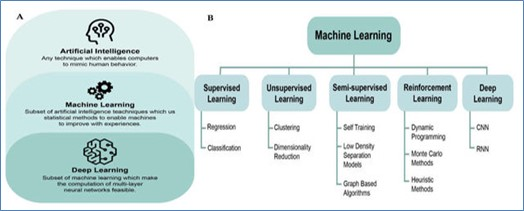
\includegraphics[width=1\columnwidth]{bab2/Gambar/Picture1.jpg}
	\end{center}
	\vspace{-0.2cm}
	%\rule{\columnwidth}{0.1pt}
	\caption{(a) Hubungan Artificial Intelligence, Machine Learning, dan Deep Learning. (b) Jenis Machine Learning\\(Sumber: C. Thongprayoon et al, 2020)}\label{img:Hubungan-Artificial-Intelligence}
\end{figure}
%%%%%%%%%%%%%%%%%%%%%%%%%% GAMBAR %%%%%%%%%%%%%%%%%%%%%%%%%%%%%%

Disamping hal tersebut, \textit{artificial intelligence} (AI) memungkinkan untuk berfikir, dan salah satu bagian dari \textit{artificial intelligence} untuk dapat melihat, mengamati, dan memahami adalah komputer visi atau \textit{computer vision}. \textit{Computer vision} memungkinkan untuk komputer dan sistem memberikan informasi berarti dari gambar digital, dan visual input. 

\section{\textit{Object Detection}}
\hspace{1,2cm}\textit{Object detection} atau deteksi objek dianggap sebagai salah satu bidang penting dalam pembelajaran mendalam dan visi komputer. Deteksi objek telah ditentukan oleh banyak aplikasi dalam visi komputer, seperti pelacakan objek, pengambilan, dan pengawasan video. Deteksi objek adalah teknologi \textit{deep learning} dimana benda, manusia, bengunan, mobil, dapat dideteksi sebagai objek dalam gambar dan video (U. Arshad, 2021).

Deteksi objek untuk mengenali objek dengan kotak pembatas pada gambar, dimana dalam klasifikasi gambar, cukup mengkategorikan (mengklasifikasikan) objek pada gambar atau tidak dalam hal kemungkinan (\textit{probability}), seperti contoh pada Gambar \ref{img:Classification-Object-Detection}

%%%%%%%%%%%%%%%%%%%%%%%%%% GAMBAR %%%%%%%%%%%%%%%%%%%%%%%%%%%%%%
\begin{figure}[H]
	\vspace{-0.1cm}
	%\rule{\columnwidth}{0.1pt}
	\begin{center}
		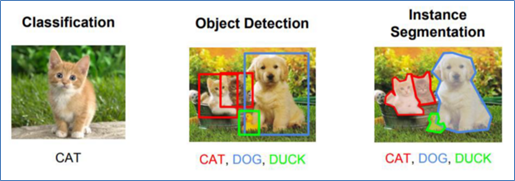
\includegraphics[width=1\columnwidth]{bab2/Gambar/Picture2.png}
	\end{center}
	\vspace{-0.2cm}
	%\rule{\columnwidth}{0.1pt}
	\caption{Classification, Object Detection dan Segmentation Representation\\(Sumber: A. Patel, 2020)}\label{img:Classification-Object-Detection}
\end{figure}
%%%%%%%%%%%%%%%%%%%%%%%%%% GAMBAR %%%%%%%%%%%%%%%%%%%%%%%%%%%%%%

Pada Gambar \ref{img:Segementation-Classification}, terlihat bahwa kucing (cat) dengan kotak pembatas dan tanpa kotak pembatas dapat membedakan mendasar antara klasifikasi citra dan deteksi objek.

%%%%%%%%%%%%%%%%%%%%%%%%%% GAMBAR %%%%%%%%%%%%%%%%%%%%%%%%%%%%%%
\begin{figure}[H]
	\vspace{-0.1cm}
	%\rule{\columnwidth}{0.1pt}
	\begin{center}
		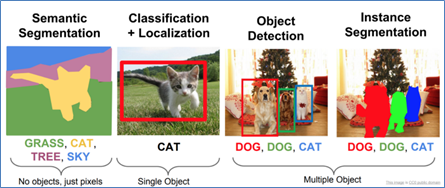
\includegraphics[width=1\columnwidth]{bab2/Gambar/Picture3.png}
	\end{center}
	\vspace{-0.2cm}
	%\rule{\columnwidth}{0.1pt}
	\caption{Segmentation, Classification+Localization, Object Detection\\(Sumber: A. Patel, 2020)}\label{img:Segementation-Classification}
\end{figure}
%%%%%%%%%%%%%%%%%%%%%%%%%% GAMBAR %%%%%%%%%%%%%%%%%%%%%%%%%%%%%%

Dalam mempelajari deteksi objek, maka diperlukan mengetahui klasifikasi citra (\textit{image classification}). Ketika gambar adalah input ke CNN, masalah mengklasifikasikan kelas yang sesuai dengan gambar dikenal sebagai klasifikasi gambar, dan seperti yang ditunjukkan pada Gambar \ref{img:Image-Classification}, nilai probabilitas untuk semua kelas yang ditargetkan adalah keluaran.

%%%%%%%%%%%%%%%%%%%%%%%%%% GAMBAR %%%%%%%%%%%%%%%%%%%%%%%%%%%%%%
\begin{figure}[H]
	\vspace{-0.1cm}
	%\rule{\columnwidth}{0.1pt}
	\begin{center}
		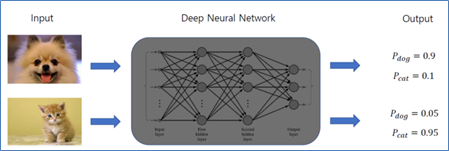
\includegraphics[width=1\columnwidth]{bab2/Gambar/Picture4.png}
	\end{center}
	\vspace{-0.2cm}
	%\rule{\columnwidth}{0.1pt}
	\caption{Image Classification\\(Sumber: A. Patel, 2020)}\label{img:Image-Classification}
\end{figure}
%%%%%%%%%%%%%%%%%%%%%%%%%% GAMBAR %%%%%%%%%%%%%%%%%%%%%%%%%%%%%%

Dapat juga dianggap bahwa deteksi objek sebagai masalah dimana tugas klasifikasi gambar memiliki tugas regresi yang memprediksi posisi objek menggunakan \textit{bounding box} (kotak pembatas) pada Gambar \ref{img:Object-Bounding-Box}. 

%%%%%%%%%%%%%%%%%%%%%%%%%% GAMBAR %%%%%%%%%%%%%%%%%%%%%%%%%%%%%%
\begin{figure}[H]
	\vspace{-0.1cm}
	%\rule{\columnwidth}{0.1pt}
	\begin{center}
		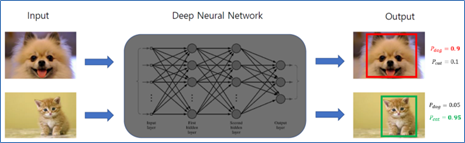
\includegraphics[width=1\columnwidth]{bab2/Gambar/Picture5.png}
	\end{center}
	\vspace{-0.2cm}
	%\rule{\columnwidth}{0.1pt}
	\caption{Object Detection dengan Bounding Box\\(Sumber: A. Patel, 2020)}\label{img:Object-Bounding-Box}
\end{figure}
%%%%%%%%%%%%%%%%%%%%%%%%%% GAMBAR %%%%%%%%%%%%%%%%%%%%%%%%%%%%%%

Masalah deteksi objek mengasumsikan bahwa beberapa kelas objek mungkin ada dalam gambar pada waktu yang sama. Dapat memvisualisasikan seperti dua jenis masalah, 1) klasifikasi multi label (beberapa kelas dalam satu gambar), 2) Bounding Box (masalah regresi) dimana harus memprediksi nilai koordinat kotak pembatas (\textit{bounding box}) dalam bentuk x, y, w, h.

Dalam deteksi objek, terdapat \textit{object localization} atau lokalisasi objek yang merupakan untuk memprediksi objek dalam sebuah citra serta batas-batasnya. Perbedaan antara lokalisasi objek dan deteksi objek tidak kentara. Sederhananya, lokalisasi objek bertujuan untuk menemukan objek utama (atau yang paling terlihat) dalam sebuah gambar, sedangkan deteksi objek mencoba untuk mengetahui semua objek dan batasannya.

Suatu klasifikasi citra atau model pengenalan citra hanya mendeteksi probabilitas suatu objek dalam suatu citra. Berbeda dengan ini, lokalisasi objek mengacu pada mengidentifikasi lokasi suatu objek dalam gambar. Algoritma lokalisasi objek akan menampilkan koordinat lokasi objek sehubungan dengan gambar. Dalam visi komputer, cara paling popular untuk melokalkan objek dalam gambar adalah dengan merepresentasikan lokasinya dengan bantuan kotak pembatas (\textit{bounding box}).

Bounding box dapat diinisialisasi menggunakan parameter berikut: 
\begin{itemize}
	\item bx, by: koordinat pusat kotak pembatas (center of bounding box)
	\item bw: lebar kotak pembatas dengan lebar gambar (width)
	\item bh: tinggi kotak pembatas dengan tinggi gambar (height)
\end{itemize}

%%%%%%%%%%%%%%%%%%%%%%%%%% GAMBAR %%%%%%%%%%%%%%%%%%%%%%%%%%%%%%
\begin{figure}[H]
	\vspace{-0.1cm}
	%\rule{\columnwidth}{0.1pt}
	\begin{center}
		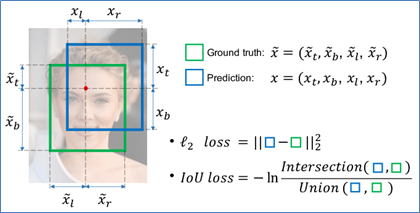
\includegraphics[width=1\columnwidth]{bab2/Gambar/Picture6.png}
	\end{center}
	\vspace{-0.2cm}
	%\rule{\columnwidth}{0.1pt}
	\caption{Intersection Over Union (IoU)\\(Sumber: A. Patel, 2020)}\label{img:Intersection-Over-Union}
\end{figure}
%%%%%%%%%%%%%%%%%%%%%%%%%% GAMBAR %%%%%%%%%%%%%%%%%%%%%%%%%%%%%%

Dengan memprediksi ini, dapat menghitung Mean-IoU dan memprediksi kotak pembatas (\textit{bounding box}) yang melokalkan objek di gambar.
\begin{itemize}
	\item IoU adalah Intersection-Over-Union (IoU) disebut sebagai Indeks Jaccard (\textit{Jaccard Index}) dianggap sebagai salah satu metrik kinerja yang paling banyak digunakan dalam deteksi objek. 

%%%%%%%%%%%%%%%%%%%%%%%%%% GAMBAR %%%%%%%%%%%%%%%%%%%%%%%%%%%%%%
\begin{figure}[H]
	\vspace{-0.1cm}
	%\rule{\columnwidth}{0.1pt}
	\begin{center}
		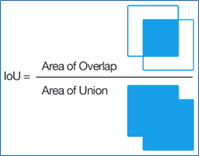
\includegraphics[width=0.4\columnwidth]{bab2/Gambar/Picture7.png}
	\end{center}
	\vspace{-0.2cm}
	%\rule{\columnwidth}{0.1pt}
	\caption{Persamaan IoU\\(Sumber: A. Patel, 2020)}\label{img:Persamaan-IOU}
\end{figure}
%%%%%%%%%%%%%%%%%%%%%%%%%% GAMBAR %%%%%%%%%%%%%%%%%%%%%%%%%%%%%%

	\item IoU adalah area tumpang tindih (\textit{overlap}) antara segmentasi yang diprediksi (\textit{prediction}) dan kebenaran dasar (\textit{ground truth}), seperti yang ditampilkan pada Gambar \ref{img:Persamaan-IOU}. Metrik ini bervariasi dari 0-1 (0-100\%) dengan 0 menyiratkan tidak ada tumpeng tindih (sampah) dan 1 menandakan segmentasi yang tumpang tindih sempurna (\textit{fat dub}).
	
	\item Mean IoU adalah segmentasi biner (dua kelas) atau multi-kelas, mean Io Udari gambar dihitung dengan mengambil IoU dari setiap kelas dan merata-ratakannya. 

\end{itemize}

\section{Machine Learning}
\hspace{1,2cm}Istilah \textit{machine learning} mula-mula diperkenalkan oleh Arthur Samuel pada tahun 1959 melalui jurnalnya yang berjudul "Some Studies in Machine Learning Using the Game of Checkers". (IBM Journal of Research and Development). Samuel mencoba mengajari program komputer untuk bermain catur. Tujuannya adalah membuat agar komputer dapat bermain catur lebih baik dari dirinya. Pada tahun 1962 program buatannya dapat mengalahkan juara catur dari negara bagian Connecticut (R. Primartha, 2018).

\textit{Machine learning} membutuhkan sebuah model yang didefinisikan berdasar parameter-parameter tertentu. Proses learning adalah eksekusi program komputer untuk mengoptimasi parameter-parameter dari model tersebut, dengan memanfaatkan data training atau \textit{past experience}.

Jadi, secara sederhana dapat dijelaskan bahwa \textit{machine learning} adalah pemrograman komputer untuk mencapai kriteria/performa tertentu dengan menggunakan sekumpulan data training atau pengalaman di masa lalu (\textit{past experience}). \textit{Machine learning} mempelajari teori agar komputer mampu "belajar" dari data. 

Secara umum algoritma \textit{machine learning} dapat dikelompokkan menjadi lima bagian, yaitu \textit{supervised learning}, \textit{unsupervised learning}, \textit{semi-supervised learning}, \textit{reinforcement learning}, dan \textit{deep learning}.

\subsection{Supervised Learning} 
\hspace{1,2cm}Sebagian besar praktik machine learning mengandalkan algoritma \textit{supervised learning}. Algoritmanya dinamakan seperti ini karena training dataset (sekumpulan data untuk training) akan memandu dan mengajari komputer agar menghasilkan outcome sesuai harapan. Pada \textit{supervised learning} menggunakan sebuah algoritma untuk mempelajari mapping function antara input dengan output. Berbagai kemungkinan output sudah diketahui dan data-data yang digunakan untuk latihan (training) sudah diberi label dengan jawaban yang benar. \textit{Supervised learning} dapat bermanfaat untuk memprediksi sesuatu dengan bantuan training dataset. Berikut skema \textit{supervised learning} pada Gambar \ref{img:Skema-Supervised-Learning} (R. Primartha, 2018).

%%%%%%%%%%%%%%%%%%%%%%%%%% GAMBAR %%%%%%%%%%%%%%%%%%%%%%%%%%%%%%
\begin{figure}[H]
	\vspace{-0.1cm}
	%\rule{\columnwidth}{0.1pt}
	\begin{center}
		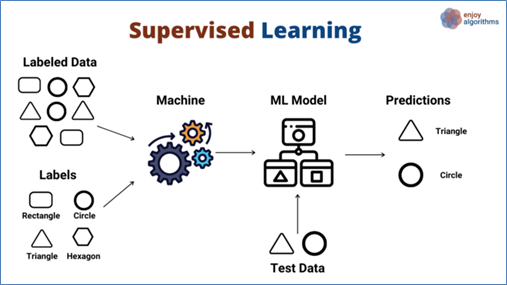
\includegraphics[width=1\columnwidth]{bab2/Gambar/Picture8.png}
	\end{center}
	\vspace{-0.2cm}
	%\rule{\columnwidth}{0.1pt}
	\caption{Skema Supervised Learning\\(Sumber: M. Kozan, 2021)}\label{img:Skema-Supervised-Learning}
\end{figure}
%%%%%%%%%%%%%%%%%%%%%%%%%% GAMBAR %%%%%%%%%%%%%%%%%%%%%%%%%%%%%%

\textit{Supervise learning} menggunakan training data yang sudah diberi label untuk mempelajari \textit{mapping function}, dari input variables (x) ke ouput variables (y).
\[y=f\ (x)\]

Sebagai contoh, sebuah algoritma klasifikasi akan dapat mengidentifikasi berbagai bentuk bangun setelah melalui proses belajar dari sekumpulan bangun datar yang sudah ditandai atau diberi label dengan ciri tertentu seperti pada gambar 2.12.

Permasalahan-permasalahan yang terkait dengan \textit{supervised learning} dapat dikategorikan menjadi dua jenis:
\begin{enumerate}
	\item \textit{Classification}
	
	Klasifikasi bertujuan untuk memprediksi outcome dari input (sample yang diberikan), dimana output variabel berbentuk kategori-kategori. Contoh: pria/wanita, sakit/sehat, tinggi/rendah, dan sebagainya.
	
	\item \textit{Regression}
	
	Regression bertujuan untuk memprediksi outcome dari input (sample yang diberikan), dimana output, variabel berbentuk nilai aktual (\textit{real values}). Contoh: prediksi harga rumah, tinggi badan seseorang, curah hujan, dan sebagainya. 
	
\end{enumerate}

Ada beberapa algoritma yang sudah dikembangkan dan terkait dengan \textit{supervised learning}, diantaranya:
\begin{enumerate}
	\item Decision tree,
	\item Naïve Bayes Classifier,
	\item Artificial Neural Network,
	\item Support Vector Machine,
	\item Linear Regression,
	\item Logistic Regression,
	\item CART,
	\item KNN (-KNearest Neighbor), dsb.
\end{enumerate}

\subsection{Unsupervised Learning}
\hspace{1,2cm}Berbeda dengan supervised learning, pada \textit{unsupervised learning} persoalan diproses hanya mengandalkan data yang belum dilatih sebelumnya. \textit{Unsepervised learning} menggunakan \textit{unlabeled training dataset} untuk memodelkan struktur dari data, sehingga unsupervised learning bersifat lebih subjektif dibandingkan \textit{supervised learning}. Berikut skema \textit{unsupervised learning} pada Gambar \ref{img:Skema-Unsupervised-Learning} (R. Primartha, 2018).

%%%%%%%%%%%%%%%%%%%%%%%%%% GAMBAR %%%%%%%%%%%%%%%%%%%%%%%%%%%%%%
\begin{figure}[H]
	\vspace{-0.1cm}
	%\rule{\columnwidth}{0.1pt}
	\begin{center}
		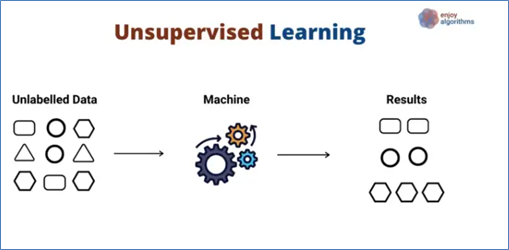
\includegraphics[width=1\columnwidth]{bab2/Gambar/Picture9.png}
	\end{center}
	\vspace{-0.2cm}
	%\rule{\columnwidth}{0.1pt}
	\caption{Skema Unsupervised Learning\\(Sumber: M. Kozan, 2021)}\label{img:Skema-Unsupervised-Learning}
\end{figure}
%%%%%%%%%%%%%%%%%%%%%%%%%% GAMBAR %%%%%%%%%%%%%%%%%%%%%%%%%%%%%%

\textit{Unsupervised learning} bermanfaat untuk kasus-kasus dimana kita ingin menemukan relasi implisit (implicit relationships) dari \textit{unlabeled dataset} yang disediakan. Jadi, pada \textit{unsupervised learning} kita tidak memprediksi masa depan, sebab input variable (X) tidak memiliki relasi dengan output variabel (Y). 
\[ f(x) \]

Untuk memudahkan memahaminya, dapat diasumsikan saat ini belum pernah membeli majalah sama sekali. Suatu ketika membeli beberapa buah majalah dan ingin membaginya menjadi beberapa kategori, dengan tujuan agar nantinya mudah dicari. Maka, dapat dimulai dengan mengidentifikasi majalah-majalah berdasarkan kemiripan. Misalnya, berdasarkan isi, penerbit, dan lain-lain yang bisa ditentukan sesuai kebutuhan.

Permasalahan seputar \textit{unsupervised learning} dapat dikelompokkan menjadi tiga kategori, yaitu:

\begin{enumerate}
	\item Association
	
	Association bertujuan untuk menemukan peluang (probabilitas) berdasarkan keterkaitan (co-occurrence) dari item-item dalam sebuah kumpulan. Sebuah contoh, jika customer membeli teh celup, maka kemungkinan besar (sekitar 80%) customer juga membeli gula pasir. Association banyak digunakan dalam market-basket analisis. 
	\item Clustering
	
	Clustering bertujuan untuk mengelompokkan sample dalam cluster yang sama berdasarkan kemiripan (similiarity).
	
	\item Dimensionality Reduction
	
	Dimensionality Reduction berarti mengurangi sejumlah variabel dari dataset namun tetap memastikan informasi yang penting masih tersedia. Dimensionality Reduction dapat diwujudkan menggunakan metode:
	\begin{enumerate}[label=(\alph*)]
		\item Feature Extraction
		
		Melakukan transformasi data dari dimensi tinggi (a high-dimensional space) ke dimensi yang lebih rendah (a low-dimensional space).
		
		\item Feature Selection
		
		Memilih Sebagian saja (subset) dari variabel asal (original variabel). 
	\end{enumerate}
\end{enumerate}

Beberapa algoritma yang dikelompokkan dalam \textit{unsupervised learning}, antara lain: 
\begin{enumerate}
	\item K-Means
	\item Hierarchical Clustering
	\item DBSCAN
	\item Fuzzy C-Means
	\item Self-Orginizing Map, dan sebagainya.	
	
\end{enumerate}

\subsection{Semi-supervised learning}
\hspace{1,2cm}Metode ini berada diantara yang \textit{supervised} dan \textit{unsupervised learning} di mana memiliki sejumlah besar masukan data, beberapa di antaranya diberi label dan sisanya tidak. Banyak masalah pembelajaran kehidupan nyata termasuk dalam bidang pembelajaran mesin ini. Alasannya adalah \textit{semi-supervised} membutuhkan lebih sedikit intervensi manusia karena menggunakan data berlabel dalam jumlah yang sangat kecil dan data yang tidak berlabel dalam jumlah besar. Memanfaatkan kumpulan data yang kurang berlabel lebih menarik karena kumpulan data tersebut sangat sulit untuk dikumpulkan serta mahal dan mungkin memerlukan akses ke pakar domain. Dataset yang tidak berlabel di sisi lain lebih murah dan lebih mudah diakses (X. Zhu, 2018).

Kedua teknik pembelajaran \textit{supervised} dan \textit{unsupervised learning} bisa digunakan untuk melatih algoritma pembelajaran dalam pembelajaran \textit{semi-supervised}. Teknik \textit{unsupervised learning} dapat digunakan untuk mengungkap struktur dan pola tersembunyi dalam kumpulan data input. Sedangkan teknik supervised learning dapat digunakan untuk membuat prediksi tebakan pada data yang tidak berlabel, memasukkan data kembali ke algoritma pembelajaran sebagai data pelatihan, dan menggunakan pengetahuan yang diperoleh untuk membuat prediksi pada kumpulan data baru. Dengan demikian, dapat mengatakan bahwa data yang tidak berlabel digunakan untuk memodifikasi atau memprioritaskan kembali prediksi atau hipotesis yang diperoleh dari data yang berlabel. Gambar \ref{img:Skema-Semi-Supervised-Learning} mengilustrasikan berbagai tahapan metode \textit{semi-supervised learning}.

%%%%%%%%%%%%%%%%%%%%%%%%%% GAMBAR %%%%%%%%%%%%%%%%%%%%%%%%%%%%%%
\begin{figure}[H]
	\vspace{-0.1cm}
	%\rule{\columnwidth}{0.1pt}
	\begin{center}
		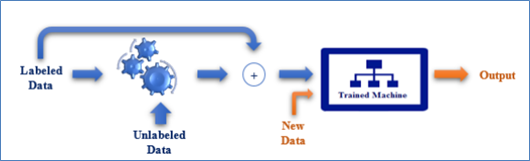
\includegraphics[width=1\columnwidth]{bab2/Gambar/Picture10.png}
	\end{center}
	\vspace{-0.2cm}
	%\rule{\columnwidth}{0.1pt}
	\captionsetup{justification=centering}
	\caption{Skema Semi-Supervised Learning\\(Sumber: \citep{SpeechRecognitionUsingDeepNeuralNetworks}}\label{img:Skema-Semi-Supervised-Learning}
\end{figure}
%%%%%%%%%%%%%%%%%%%%%%%%%% GAMBAR %%%%%%%%%%%%%%%%%%%%%%%%%%%%%%

Untuk memanfaatkan data pelatihan yang tidak berlabel, semua algoritma \textit{semi-supervised learning} melakukan setidaknya satu dari asumsi berikut asumsi kehalusan, asumsi cluster, dan asumsi manifold.

\subsection{Reinforcement Learning}
\hspace{1,2cm}\textit{Reinforcement learning} merupakan metode pembelajaran yang dipengaruhi oleh feedback dari lingkungan dengan Teknik pembelajaran yang iterative (berulang-ulang) dan adaptive (menyesuaikan). \textit{Reinforcement learning} dipercaya mendekati cara manusia belajar (R. Primartha, 2018). 

\textit{Reinforcement learning} (RL) diinspirasi oleh kebiasaan makhluk hidup dalam belajar dan bertindak, khususnya manusia. Pada RL tidak ada dataset. Data-data diperoleh berdasarkan pengalaman. Algoritma \textit{reinforcement learning} mengijinkan agent untuk memutuskan aksi selanjutnya berdasarkan kondisi saat ini (\textit{current state}). \textit{Reinforcement learning} kadang disebut juga \textit{credit assessment learning}, sebab learning difokuskan untuk memaksimalkan perolehan \textit{rewards}. \textit{Reinforcement learning} tergantung pada proses coba-coba untuk mengungkap rangkaian tindakan yang memaksimalkan metrik imbalan kumulatif, yang digunakan untuk membuat algoritma memahami apakah itu mengarah ke arah yang benar atau tidak. Berikut skema \textit{reinforcement learning} pada Gambar \ref{img:Skema-Reinforcement-Learning}. 

%%%%%%%%%%%%%%%%%%%%%%%%%% GAMBAR %%%%%%%%%%%%%%%%%%%%%%%%%%%%%%
\begin{figure}[H]
	\vspace{-0.1cm}
	%\rule{\columnwidth}{0.1pt}
	\begin{center}
		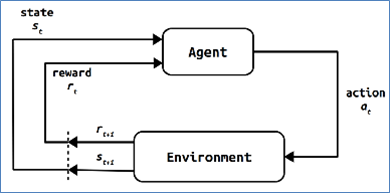
\includegraphics[width=1\columnwidth]{bab2/Gambar/Picture11.png}
	\end{center}
	\vspace{-0.2cm}
	%\rule{\columnwidth}{0.1pt}
	\captionsetup{justification=centering}
	\caption{Skema Reinforcement Learning\\(Sumber: R. Sutton, 1998)}\label{img:Skema-Reinforcement-Learning}
\end{figure}
%%%%%%%%%%%%%%%%%%%%%%%%%% GAMBAR %%%%%%%%%%%%%%%%%%%%%%%%%%%%%%

Menurut R. Sutton, proses \textit{reinforcement learning} dapat dipresentasikan dalam matematika sebagai \textit{Markov Decision Process} (MDP), memperkenalkan 4 set {S, A, P, R}, dengan:\\
S - Kumpulan status tempat agen dapat berada, pada saat tertentu;\\
A - Serangkaian kemungkinan Tindakan yang dapat dilakukan agen dalam waktu tertentu;\\
P - Himpunan probabilitas, bahwa sebuah agen, yang berada dalam keadaan s, bertransisi ke keadaan s' dengan melakukan Tindakan A dalam waktu t+1;

Representasi \textit{reinforcement learning} mirip dengan supervised learning. Yang membedakan adalah pada reinforcement learning tidak hanya x, namun x dan z.
\[ y=\ f\ \left(x\right)\ given\ z \]

Tidak seperti \textit{supervised} dan \textit{unsupervised learning} dimana algoritma sudah memiliki tujuan (goal). Algoritma \textit{reinforcement learning} tidak memiliki tujuan eksplisit, sebagai gantinya algoritma dipaksa untuk belajar menemukan nilai optimal melalui kegiatan trial dan error.

\textit{Reinforcement learning} banyak diimplementasikan pada \textit{game theory, control theory, operation research, information theory, simulation-based optimaztion, multi-agent systems, swarm intelligence, statistics}, dan \textit{genetic algorithm}.

Contoh penerapan \textit{reinforcement learning} yaitu pada bidang robotic. Sebuah robot dapat belajar untuk menghindari tabrakan dengan cara menerima feedback negative manakala robot tersebut menabrak halangan tertentu. Robot akan dibiarkan berjalan tanpa dipandu. Robot akan belajar dari pengalaman sebelumnya untuk menemukan rute paling optimal. 

Beberapa algoritma yang dikelompokkan dalam \textit{reinforcement learning} antara lain:
\begin{enumerate}
	\item Genetic Algorithm (GA)
	\item Dynamic Programming (DP)
	\item Generalized Policy Iteration (GPI)
	\item Monte Carlo Methods
\end{enumerate}

\subsection{Deep Learning}
\hspace{1,2cm}\textit{Deep learning} merupakan metode pembelajaran yang memanfaatkan \textit{artificial neural networks} yang berlapis-lapis (multi layer). \textit{Artificial neural networks} ini dibuat mirip dengan otak manusia, di mana neuron-neuron terkoneksi satu sama lain, sehingga membentuk sebuah jaringan neuron yang sangat rumit (R. Primartha, 2018).

\textit{Deep learning} atau \textit{deep structured leaning} atau hierarchical learning atau deep neural merupakan metode pembelajaran yang memanfaatkan multiple non-linear transformation. \textit{Deep learning} dapat dipandang sebagai gabungan machine learning dengan \textit{artificial intelligence} (AI). \textit{Deep learning} pada hakekatnya merupakan perluasan atau pengembangan dari \textit{neural network} atau jaringan saraf tiruan (JST).

Jika dikembalikan kepada tujuan \textit{machine learning} semula, yaitu komputer yang dapat belajar (dari data atau pengalaman), maka \textit{deep learning} adalah apa yang selama ini dicari. \textit{Deep learning} menirukan cara berpikir manusia. Pada \textit{deep learning}, komputer harus memproses data yang sangat banyak, berlapis-lapis, dan output dari layer sebelumnya akan menjadi input bagi layer sesudahnya.

Struktur umum dan dasar dari skema \textit{deep learning} ditunjukkan pada Gambar \ref{img:Skema-Umum-Deep-Learning}. Ini terdiri dari lapisan masukan, yang merupakan data masukan ke algoritma; lapisan tersembunyi, di mana algoritma membuat banyak perhitungan matematis, dan lapisan output, yang merupakan hasil dari perhitungan algoritma.

%%%%%%%%%%%%%%%%%%%%%%%%%% GAMBAR %%%%%%%%%%%%%%%%%%%%%%%%%%%%%%
\begin{figure}[H]
	\vspace{-0.1cm}
	%\rule{\columnwidth}{0.1pt}
	\begin{center}
		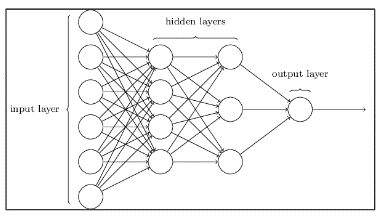
\includegraphics[width=1\columnwidth]{bab2/Gambar/Picture12.png}
	\end{center}
	\vspace{-0.2cm}
	%\rule{\columnwidth}{0.1pt}
	\captionsetup{justification=centering}
	\caption{Skema Umum \textit{Deep Learning}\\(Sumber: A. Feizollah et al, 2022)}\label{img:Skema-Umum-Deep-Learning}
\end{figure}
%%%%%%%%%%%%%%%%%%%%%%%%%% GAMBAR %%%%%%%%%%%%%%%%%%%%%%%%%%%%%%
Sejarah \textit{deep learning} dimulai pada tahun 2006, yaitu setelah Geoffrey Hinton mempublikasikan paper yang memperkenalkan salah satu varian \textit{neural networks} yang disebut \textit{deep belief nets}. Paper ini merupakan awal kemunculan istilah \textit{deep learning}, untuk membedakan arsitektur \textit{neural network} konvensional (\textit{single layer}) dengan arsitektur neural network multi/banyak layer. Dengan kata lain, deep learning adalah salah satu cabang machine learning yang menggunakan \textit{deep neural network} untuk menyelesaikan permasalahan pada domain \textit{machine learning}. 

Pada tahun 2009, Andrew memperkenalkan penggunaan GPU untuk \textit{deep learning} melalui paper yang berjudul \textit{large-scale deep unsupervised learning using graphics processors}. Dengan menggunakan GPU, algoritma \textit{deep learning} dapat dijalankan lebih cepat disbanding dengan tanpa GPU (hanya menggunakan CPU), Perkembangan \textit{deep learning} maju pesat berkat keberadaan \textit{hardware} yang memadai. Dan saat ini, \textit{deep learning} sudah banyak diaplikasikan di berbagai area, seperti pengenal wajah, \textit{self-driving car}, pengenal suara, dan sebagainya. 

\textit{Deep learning} merupakan jalan untuk mencapai apa yang sudah dicita-citakan sebelumnya oleh manusia, yaitu kecerdasan buatan bagi mesin. Bentuk diagram \textit{network model deep learning} seperti pada Gambar \ref{img:Skema-Deep-Learning-Hidden-Layer}. Perhatikan bahwa \textit{hidden layer} hanya digambarkan tiga lapis saja, padahal kenyataanya bisa berjumlah sangat banyak, dapat diasumsikan seperti Gambar \ref{img:Skema-Deep-Learning-Hidden-Layer}.

%%%%%%%%%%%%%%%%%%%%%%%%%% GAMBAR %%%%%%%%%%%%%%%%%%%%%%%%%%%%%%
\begin{figure}[H]
	\vspace{-0.1cm}
	%\rule{\columnwidth}{0.1pt}
	\begin{center}
		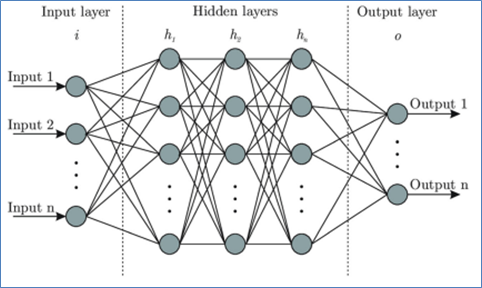
\includegraphics[width=1\columnwidth]{bab2/Gambar/Picture13.png}
	\end{center}
	\vspace{-0.2cm}
	%\rule{\columnwidth}{0.1pt}
	\captionsetup{justification=centering}
	\caption{Skema \textit{Deep Learning} dengan Penambahan beberapa \textit{hidden layer}\\(Sumber: H. Kaur et al, 2021)}\label{img:Skema-Deep-Learning-Hidden-Layer}
\end{figure}
%%%%%%%%%%%%%%%%%%%%%%%%%% GAMBAR %%%%%%%%%%%%%%%%%%%%%%%%%%%%%%

Pada Gambar \ref{img:Skema-Deep-Learning-Hidden-Layer} mengandung 3 layer, yaitu input, \textit{hidden} dan output layer. Penambahan \textit{layer} ini terjadi pada \textit{hidden layer}. \textit{Hidden layer} pada skema \textit{deep learning} yang disebut dengan \textit{Multi Layer Peceptron} (MLP) disebabkan jumlah neuron semakin banyak dan itu artinya semakin banyak juga perhitungan yang harus dikerjakan pada setiap \textit{layer}. MLP merupakan pengembangan dari \textit{Single Layer Perceptron} (SLP) yang merupakan model paling sederhana dari neural network dan sekaligus merupakan dasar bagi model-model tingkat lanjut yang digunakan pada \textit{deep learning}. MLP kemudian menjadi cikal bakal metode \textit{deep learning} atau \textit{deep neural network} (DNN).

\textit{Deep learning} sudah dikembangkan ke berbagai model atau arsitektur yang berbeda-beda. Berikut daftar beberapa model atau arsitektur untuk \textit{deep learning}. 
\begin{enumerate}
	\item \textit{Recurrent Neural Networks} (RNN)
	\item \textit{Long Short-Term Memory} (LSTM)
	\item \textit{Convolutional Neural Network} (CNN)
	\item \textit{Deep Believe Networks} (DBN)
	\item \textit{Deep Stacking Networks} (DSN)
\end{enumerate}

Contoh penerapan masing-masing arsitektur deep learning dapat dipelajari pada Tabel \ref{tbl:Penerapan-Arsitektur-Deep-Learning}
%%%%%%%%%%%%%%%%%%%%%%%TABEL SEDERHANA%%%%%%%%%%%%%%%%%%%%%%%%%
\begin{singlespace}
	\begin{table}[H]
		\centering
		\caption{Penerapan Arsitektur Deep Learning}
		\label{tbl:Penerapan-Arsitektur-Deep-Learning}
		\begin{adjustbox}{width=\columnwidth,center}
			\begin{tabular}{|c|c|l|}
				\hline
				No. & Arsitektur & \multicolumn{1}{c|}{Penerapan}                                                                                                                                           \\ \hline
				1   & RNN        & \textit{Speech recognition, handwriting recognition}                                                                                                                     \\ \hline
				2   & LSTM       & \textit{\begin{tabular}[c]{@{}l@{}}Natural language text compression, handwriting recognition,\\ speech recognition, gesture recognition, image captioning\end{tabular}} \\ \hline
				3   & CNN        & \textit{Image recognition, video analysis, natural language processing}                                                                                                  \\ \hline
				4   & DBN        & \textit{\begin{tabular}[c]{@{}l@{}}Image recognition, information retrieval, \\ natural language understanding, failure prediction\end{tabular}}                         \\ \hline
				5   & DSN        & \textit{Information retrieval, continuous speech recognition}                                                                                                            \\ \hline
			\end{tabular}
		\end{adjustbox}
	\end{table}
\end{singlespace}
%%%%%%%%%%%%%%%%%%%%%%%TABEL SEDERHANA%%%%%%%%%%%%%%%%%%%%%%%%%
Masing-masing arsitektur pada Tabel \ref{tbl:Penerapan-Arsitektur-Deep-Learning} memiliki perbedaan, berikut penjelasan dan diagram network beberapa arsitektur deep learning yang umum.

\subsubsection{Recurrent Neural Networks (RNN)}
\hspace{1,2cm}\textit{Recurrent Neural Network} (RNN) merupakan arsitektur \textit{deep learning} yang popular serta sangat menjanjinak untuk menyelesaikan berbagai persoalan yang terkait dengan \textit{Natural Language Processing} (NLP). Model RNN digunakan agar mesin dapat memahami bahasa manusia. Mulai dari cara berkomunikasi, mendengarkan, mengenali percakapan, hingga memahami tata bahasa dan aksen. RNN juga dapat diimplementasikan untuk mengenali gambar-gambar atau objek (R. Primartha, 2018).

Diagram network RNN seperti pada Gambar \ref{img:Diagram-RNN} berikut. 
%%%%%%%%%%%%%%%%%%%%%%%%%% GAMBAR %%%%%%%%%%%%%%%%%%%%%%%%%%%%%%
\begin{figure}[H]
	\vspace{-0.1cm}
	%\rule{\columnwidth}{0.1pt}
	\begin{center}
		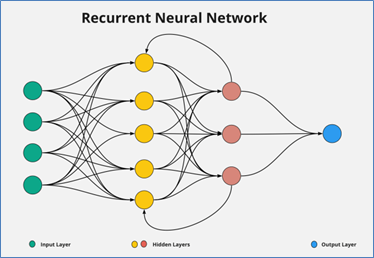
\includegraphics[width=0.8\columnwidth]{bab2/Gambar/Picture14.png}
	\end{center}
	\vspace{-0.2cm}
	%\rule{\columnwidth}{0.1pt}
	\captionsetup{justification=centering}
	\caption{Diagram \textit{Recurent Neural Network} (RNN)\\(Sumber: K. Dass, 2020)}\label{img:Diagram-RNN}
\end{figure}
%%%%%%%%%%%%%%%%%%%%%%%%%% GAMBAR %%%%%%%%%%%%%%%%%%%%%%%%%%%%%%

\subsubsection{Long Short Term Memory (LSTM)}
\hspace{1,2cm}\textit{Long Short Term Memory} (LSTM) merupakan building unit untuk \textit{layer-layer} pada recurrent neural network (RNN). LSTM mula-mula diusulkan oleh Sepp Hochreiter dan Jurgen Schmidhuber pada tahun 1997. LSTM juga banyak diimplementasikan pada bidang NLP. Boleh dibilang LSTM merupakan pengembangan dari RNN. Secara teoritis, jaringan saraf yang terhubung secara naif, yang disebut jaringan saraf berulang, dapat bekerja. Namun dalam praktiknya, mengalami dua masalah: gradien menghilang dan gradien meledak, yang membuatnya tidak dapat digunakan (R. Primartha, 2018).  Kemudian, LSTM ditemukan untuk mengatasi masalah ini dengan secara eksplisit memasukkan unit memori, yang disebut sel ke dalam jaringan. Ini adalah diagram blok bangunan LSTM pada Gambar \ref{img:Diagram-LSTM}.

%%%%%%%%%%%%%%%%%%%%%%%%%% GAMBAR %%%%%%%%%%%%%%%%%%%%%%%%%%%%%%
\begin{figure}[H]
	\vspace{-0.1cm}
	%\rule{\columnwidth}{0.1pt}
	\begin{center}
		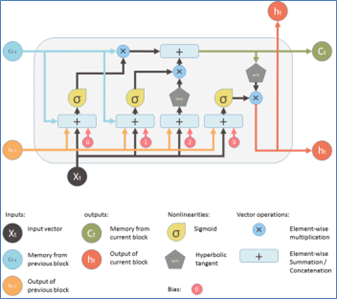
\includegraphics[width=0.8\columnwidth]{bab2/Gambar/Picture15.png}
	\end{center}
	\vspace{-0.2cm}
	%\rule{\columnwidth}{0.1pt}
	\captionsetup{justification=centering}
	\caption{Diagram \textit{Long Short Term Memory} (LSTM) \\(Sumber: S. Yan, 2016)}\label{img:Diagram-LSTM}
\end{figure}
%%%%%%%%%%%%%%%%%%%%%%%%%% GAMBAR %%%%%%%%%%%%%%%%%%%%%%%%%%%%%%

\subsubsection{Convolutional Neural Network (CNN)}
\hspace{1,2cm}\textit{Convolutional Neural Networks} (CNN atau ConvNet) merupakan salah satu model deep learning yang banyak digunakan untuk keperluan analisis citra/visual. CNN adalah salah satu kategori utama untuk melakukan pengenalan dan klasifikasi gambar, deteksi objek, pengenalan wajah, dan sebagainya merupakan beberapa area dimana CNN banyak digunakan (R. Primartha, 2018).

Klasifikasi gambar CNN mengambil input gambar, memproses, dan mengklasifikasikannya dalam kategori tertentu, misalnya kucing, harimau, singa. Komputer melihat gambar input sebagai susunan piksel dan itu tergantung pada resolusi gambar. Berdasarkan resolusi gambar, akan terlihat h x w x d (h = Tinggi, w = Lebar, d = Dimensi). Misalnya, gambar array matriks RGB 6 x 6 x 3 (3 mengacu pada nilai RGB) dan gambar array matriks 4 x 4 x 1 dari gambar skala abu-abu, seperti pada Gambar \ref{img:Array-Matriks-RGB}.

%%%%%%%%%%%%%%%%%%%%%%%%%% GAMBAR %%%%%%%%%%%%%%%%%%%%%%%%%%%%%%
\begin{figure}[H]
	\vspace{-0.1cm}
	%\rule{\columnwidth}{0.1pt}
	\begin{center}
		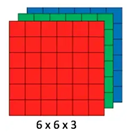
\includegraphics[width=0.3\columnwidth]{bab2/Gambar/Picture16.png}
	\end{center}
	\vspace{-0.2cm}
	%\rule{\columnwidth}{0.1pt}
	\captionsetup{justification=centering}
	\caption{Array dari Matriks RGB\\(Sumber: R. Prabhu, 2018)}\label{img:Array-Matriks-RGB}
\end{figure}
%%%%%%%%%%%%%%%%%%%%%%%%%% GAMBAR %%%%%%%%%%%%%%%%%%%%%%%%%%%%%%

Secara teknis, model \textit{deep learning} CNN untuk latih dan uji, setiap gambar input akan melewati serangkaian lapisan konvolusi dengan filter (Kernel), Pooling, \textit{fully connected layers} (FC) dan menerapkan fungsi softmax untuk mengklasifikasikan objek dengan nilai probabilistic antara 0 dan 1. Gambar 2.17. adalah alur dari CNN untuk memproses gambar input dan mengklasifikasikan objek berdasarkan nilai.


%%%%%%%%%%%%%%%%%%%%%%%%%% GAMBAR %%%%%%%%%%%%%%%%%%%%%%%%%%%%%%
\begin{figure}[H]
	\vspace{-0.1cm}
	%\rule{\columnwidth}{0.1pt}
	\begin{center}
		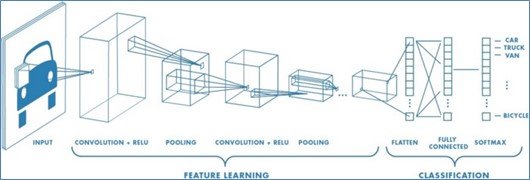
\includegraphics[width=1\columnwidth]{bab2/Gambar/Picture17.jpg}
	\end{center}
	\vspace{-0.2cm}
	%\rule{\columnwidth}{0.1pt}
	\captionsetup{justification=centering}
	\caption{Neural Network dengan banyak Convolusi Layer\\(Sumber: R. Prabhu, 2018)}\label{img:Neural-Network-Dengan-Banyak-Convolusi-Layer}
\end{figure}
%%%%%%%%%%%%%%%%%%%%%%%%%% GAMBAR %%%%%%%%%%%%%%%%%%%%%%%%%%%%%%

\begin{enumerate}
	\item \textit{Convolution Layer}
	
	Konvolusi adalah lapisan pertama untuk mengekstraksi fitur dari gambar masukan. Konvolusi mempertahankan hubungan antara piksel dengan mempelajari fitur gambar menggunakan kotak kecil data masukan. Ini adalah operasi matematika yang mengambil dua input, seperti matriks gambar dan filter atau kernel.
	
	\begin{itemize}
		\item Sebuah gambar matriks (volume) dari dimensi \textbf{(h x w x d)}
		\item Sebuah filter \textbf{(fh x fw x d)}
		\item Output volume dimensi \textbf{(h - fh + 1) x (w - fw + 1) x 1 }
		
		%%%%%%%%%%%%%%%%%%%%%%%%%% GAMBAR %%%%%%%%%%%%%%%%%%%%%%%%%%%%%%
		\begin{figure}[H]
			\vspace{-0.1cm}
			%\rule{\columnwidth}{0.1pt}
			\begin{center}
				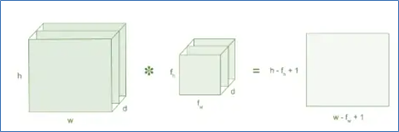
\includegraphics[width=1\columnwidth]{bab2/Gambar/Picture18.png}
			\end{center}
			\vspace{-0.2cm}
			%\rule{\columnwidth}{0.1pt}
			\captionsetup{justification=centering}
			\caption{Gambar Matriks Multiplies Kernel atau Filter Matriks\\(Sumber: R. Prabhu, 2018)}\label{img:Matriks-Multiplies}
		\end{figure}
		%%%%%%%%%%%%%%%%%%%%%%%%%% GAMBAR %%%%%%%%%%%%%%%%%%%%%%%%%%%%%%
	\end{itemize}
	Pertimbangkan gambar 5 x 5 yang nilai piksel gambarnya adalah 0, 1 dan matriks filter 3 x 3, seperti pada Gambar \ref{img:Matriks5x5}.
	
	%%%%%%%%%%%%%%%%%%%%%%%%%% GAMBAR %%%%%%%%%%%%%%%%%%%%%%%%%%%%%%
	\begin{figure}[H]
		\vspace{-0.1cm}
		%\rule{\columnwidth}{0.1pt}
		\begin{center}
			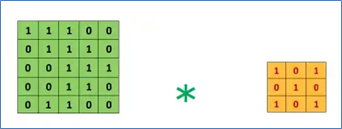
\includegraphics[width=0.7\columnwidth]{bab2/Gambar/Picture19.png}
		\end{center}
		\vspace{-0.2cm}
		%\rule{\columnwidth}{0.1pt}
		\captionsetup{justification=centering}
		\caption{Gambar matriks 5 x 5 dikalikan dengan Filter matiks 3 x 3}\label{img:Matriks5x5}
	\end{figure}
	%%%%%%%%%%%%%%%%%%%%%%%%%% GAMBAR %%%%%%%%%%%%%%%%%%%%%%%%%%%%%% 
	
	Kemudian, konvolusi matriks gambar 5 x 5 dikalikan dengan filter matriks 3 x 3 yang disebut "Feature Map" sebagai output yang ditunjukkan pada Gambar \ref{img:Output-Matriks-3-3}.
	
	%%%%%%%%%%%%%%%%%%%%%%%%%% GAMBAR %%%%%%%%%%%%%%%%%%%%%%%%%%%%%%
	\begin{figure}[H]
		\vspace{-0.1cm}
		%\rule{\columnwidth}{0.1pt}
		\begin{center}
			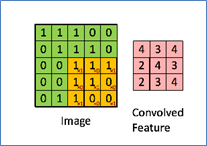
\includegraphics[width=0.7\columnwidth]{bab2/Gambar/Picture20.png}
		\end{center}
		\vspace{-0.2cm}
		%\rule{\columnwidth}{0.1pt}
		\captionsetup{justification=centering}
		\caption{Output Matriks 3 x 3}\label{img:Output-Matriks-3-3}
	\end{figure}
	%%%%%%%%%%%%%%%%%%%%%%%%%% GAMBAR %%%%%%%%%%%%%%%%%%%%%%%%%%%%%%
	
	Konvolusi gambar dengan filter berbeda dapat melakukan operasi seperti deteksi tepi, mengaburkan, dan memeprtajam dengan menerapkan filter. Berikut ini contoh yang menunjukkan berbagai gambar konvolusi setelah menerapkan berbagai jenis filter (Kernel) pada Gambar \ref{img:Fitur-Umum}.
	
	%%%%%%%%%%%%%%%%%%%%%%%%%% GAMBAR %%%%%%%%%%%%%%%%%%%%%%%%%%%%%%
	\begin{figure}[H]
		\vspace{-0.1cm}
		%\rule{\columnwidth}{0.1pt}
		\begin{center}
			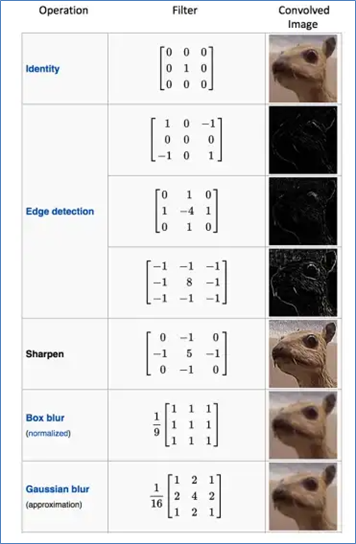
\includegraphics[width=0.6\columnwidth]{bab2/Gambar/Picture21.png}
		\end{center}
		\vspace{-0.2cm}
		%\rule{\columnwidth}{0.1pt}
		\captionsetup{justification=centering}
		\caption{Beberapa Filter Umum\\(Sumber: R. Prabhu, 2018)}\label{img:Fitur-Umum}
	\end{figure}
	%%%%%%%%%%%%%%%%%%%%%%%%%% GAMBAR %%%%%%%%%%%%%%%%%%%%%%%%%%%%%%
	
	\item Strides
	
	Stride adalah jumlah piksel yang bergeser di atas matriks input. Saat langkahnya 1, maka memindahkan filter ke 1 piksel sekaligus. Saat langkahnya 2, maka memindahkan filter ke 2 piksel sekaligus dan seterusnya. Gambar \ref{img:Stride-2-Piksel} menunjukkan konvolusi akan bekerja dengan Langkah 2.
	
	%%%%%%%%%%%%%%%%%%%%%%%%%% GAMBAR %%%%%%%%%%%%%%%%%%%%%%%%%%%%%%
	\begin{figure}[H]
		\vspace{-0.1cm}
		%\rule{\columnwidth}{0.1pt}
		\begin{center}
			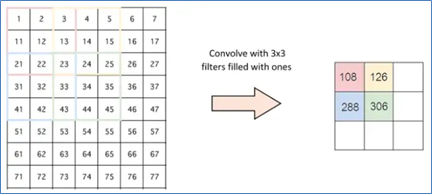
\includegraphics[width=0.6\columnwidth]{bab2/Gambar/Picture22.png}
		\end{center}
		\vspace{-0.2cm}
		%\rule{\columnwidth}{0.1pt}
		\captionsetup{justification=centering}
		\caption{Stride 2 Piksel\\(Sumber: R. Prabhu, 2018)}\label{img:Stride-2-Piksel}
	\end{figure}
	%%%%%%%%%%%%%%%%%%%%%%%%%% GAMBAR %%%%%%%%%%%%%%%%%%%%%%%%%%%%%%
	
	\item Padding
	
	Pada saat penggunaan filter, terkadang filter tidak pas dengan gambar masukan. Maka, terdapat dua pilihan: 
	\begin{itemize}
		\item Memadatkan gambar dengan angka nol (\textit{zero padding}) agar pas; 
		\item Menghilangkan bagian gambar yang tidak sesuai dengan filter. Ini disebut dengan \textit{valid padding} yang hanya menyimpan bagian gambar yang valid. 
		
	\end{itemize}
	
	\item Non Linerarity (ReLU)
	
	ReLU adalah singkatan dari \textit{Rectified Linear Unit} untuk operasi non-linear. Outputnya adalah \textit{f(x) = maks(0,x)}. ReLU penting karena tujuan ReLU adalah untuk mengenalkan non-linearitas di ConvNet, karena data dunia nyata ingin ConvNet pelajari adalah nilai linier non-negatif. Fungsi ini hanya mengembalikan nilai 0 jika nilai tersebut bernilai negative, selain itu mengembalikan nilai yang sama dengan yang diberikan, tidak lain adalah menghilangkan keluaran negative dan mempertahankan nilai antara 0 hingga + tak terhingga, seperti pada Gambar \ref{img:Operasi-RELU}. 
	
	%%%%%%%%%%%%%%%%%%%%%%%%%% GAMBAR %%%%%%%%%%%%%%%%%%%%%%%%%%%%%%
	\begin{figure}[H]
		\vspace{-0.1cm}
		%\rule{\columnwidth}{0.1pt}
		\begin{center}
			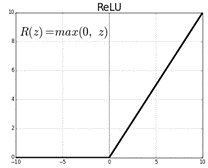
\includegraphics[width=0.3\columnwidth]{bab2/Gambar/Picture23.1.png}\\
			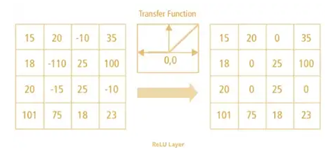
\includegraphics[width=0.6\columnwidth]{bab2/Gambar/Picture23.2.png}
		\end{center}
		\vspace{-0.2cm}
		%\rule{\columnwidth}{0.1pt}
		\captionsetup{justification=centering}
		\caption{Operasi ReLU\\(Sumber: P. Ratan, 2021)}\label{img:Operasi-RELU}
	\end{figure}
	%%%%%%%%%%%%%%%%%%%%%%%%%% GAMBAR %%%%%%%%%%%%%%%%%%%%%%%%%%%%%%
	
	\item Pooling Layer
	
	Bagian layer pooling akan mengurangi jumlah parameter ketika gambar terlalu besar. Penyatuan spasial juga disebut subsampling atau downsampling yang mengurangi dimensi setiap peta tetapi tetap mempertahankan informasi penting. Penyatuan spasial dapat dari berbagai jenis, diantaranya Max Pooling, Average Pooling, dan Sum Pooling.\\
	Max Pooling mengambil elemen tersbesar dari peta fitur yang diperbaiki. Mengambil elemen terbesar juga bisa mengambil pooling rata-rata. Jumlah semua elemen dalam peta fitur disebut sebagai kumpulan jumlah.
	
	%%%%%%%%%%%%%%%%%%%%%%%%%% GAMBAR %%%%%%%%%%%%%%%%%%%%%%%%%%%%%%
	\begin{figure}[H]
		\vspace{-0.1cm}
		%\rule{\columnwidth}{0.1pt}
		\begin{center}
			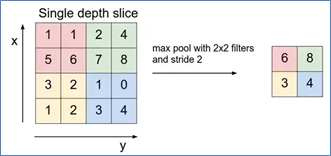
\includegraphics[width=0.5\columnwidth]{bab2/Gambar/Picture24.png}
		\end{center}
		\vspace{-0.2cm}
		%\rule{\columnwidth}{0.1pt}
		\captionsetup{justification=centering}
		\caption{Max Pooling}\label{img:Max-Polling}
	\end{figure}
	%%%%%%%%%%%%%%%%%%%%%%%%%% GAMBAR %%%%%%%%%%%%%%%%%%%%%%%%%%%%%%
	
	\item Fully Connected Layer

	Lapisan yang disebut \textit{Fully Connected Layer}, diratakan matriks menjadi vector dan memasukkannya ke dalam \textit{fully connected layer}, seperti jaringan saraf (\textit{neural network}), seperti Gambar \ref{img:Setelah-Pooling-Layer}.
	
	%%%%%%%%%%%%%%%%%%%%%%%%%% GAMBAR %%%%%%%%%%%%%%%%%%%%%%%%%%%%%%
	\begin{figure}[H]
		\vspace{-0.1cm}
		%\rule{\columnwidth}{0.1pt}
		\begin{center}
			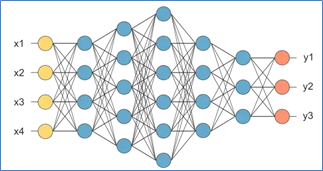
\includegraphics[width=0.5\columnwidth]{bab2/Gambar/Picture25.png}
		\end{center}
		\vspace{-0.2cm}
		%\rule{\columnwidth}{0.1pt}
		\captionsetup{justification=centering}
		\caption{Setelah Pooling Layer Diratakan sebagai FC Layer}\label{img:Setelah-Pooling-Layer}
	\end{figure}
	%%%%%%%%%%%%%%%%%%%%%%%%%% GAMBAR %%%%%%%%%%%%%%%%%%%%%%%%%%%%%%
	
	Pada Gambar \ref{img:Setelah-Pooling-Layer}, matriks peta fitur akan diubah menjadi vector (x1, x2, x3, ...). Dengan lapisan yang terhubung sepenuhnya, digabungkan fitur ini bersama untuk membuat model. Setelah itu, akhirnya memiliki fungsi aktivasi seperti softmax atau sigmoid untuk mengklasifikasikan keluaran sebagai objek, misalnya rumah, pohon, kucing, mobil, truk, dan sebagainya, seperti pada Gambar \ref{img:Arsitektur-CNN-Lengkap}.
	
	%%%%%%%%%%%%%%%%%%%%%%%%%% GAMBAR %%%%%%%%%%%%%%%%%%%%%%%%%%%%%%
	\begin{figure}[H]
		\vspace{-0.1cm}
		%\rule{\columnwidth}{0.1pt}
		\begin{center}
			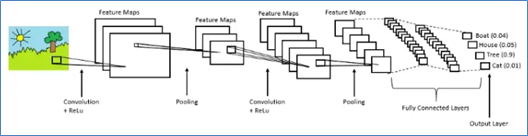
\includegraphics[width=0.5\columnwidth]{bab2/Gambar/Picture26.png}
		\end{center}
		\vspace{-0.2cm}
		%\rule{\columnwidth}{0.1pt}
		\captionsetup{justification=centering}
		\caption{Arsitektur CNN Lengkap}\label{img:Arsitektur-CNN-Lengkap}
	\end{figure}
	%%%%%%%%%%%%%%%%%%%%%%%%%% GAMBAR %%%%%%%%%%%%%%%%%%%%%%%%%%%%%%
	
\end{enumerate}

\subsubsection{Deep Believe Networks (DBN)}
\hspace{1,2cm}\textit{Deep Belief Neworks} (DBN) merupakan model \textit{deep learning} yang memanfaatkan tumpukan/\textit{stack Restricted Boltzmann Machines} (RBM) atau kadangkala \textit{Autoencoders}. \textit{Autoencoders} adalah model \textit{neural networks} yang memiliki input dan output yang sama. \textit{Autoencoder} mempelajari data input dan berusaha untuk melakukan rekonstruksi terhadap data input tersebut (R. Primartha, 2018).  Skema diagram DBN seperti pada Gambar \ref{img:Skema-Diagram-DBN}.

%%%%%%%%%%%%%%%%%%%%%%%%%% GAMBAR %%%%%%%%%%%%%%%%%%%%%%%%%%%%%%
\begin{figure}[H]
	\vspace{-0.1cm}
	%\rule{\columnwidth}{0.1pt}
	\begin{center}
		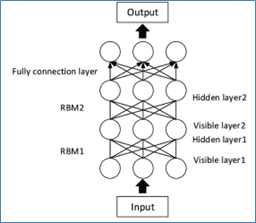
\includegraphics[width=0.6\columnwidth]{bab2/Gambar/Picture27.png}
	\end{center}
	\vspace{-0.2cm}
	%\rule{\columnwidth}{0.1pt}
	\captionsetup{justification=centering}
	\caption{Skema Diagram DBN\\(Sumber: H. Liu {\&} B. Lang, 2019)}\label{img:Skema-Diagram-DBN}
\end{figure}
%%%%%%%%%%%%%%%%%%%%%%%%%% GAMBAR %%%%%%%%%%%%%%%%%%%%%%%%%%%%%%

\subsubsection{Deep Stacking Networks (DSN)}
\hspace{1,2cm}Salah satu masalah pada \textit{deep learning} adalah proses learning sangat sulit dilakukan dan memerlukan komputasi yang cukup kompleks. Pada tahun 2011 Deng Yu mengusulkan model \textit{Deep Convex Networks} (DCN) atau \textit{Deep Stacking Network} (DSN), yang sedikit berbeda dibandingkan model \textit{deep learning} lain (R. Primartha, 2018). Secara umum model DSN terdiri atas ub-nets berukuran kecil dengan hanya sebuah hidden layer, seperti pada Gambar \ref{img:Skema-Diagram-DSN}.

%%%%%%%%%%%%%%%%%%%%%%%%%% GAMBAR %%%%%%%%%%%%%%%%%%%%%%%%%%%%%%
\begin{figure}[H]
	\vspace{-0.1cm}
	%\rule{\columnwidth}{0.1pt}
	\begin{center}
		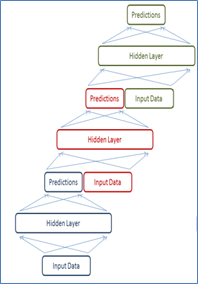
\includegraphics[width=0.4\columnwidth]{bab2/Gambar/Picture28.png}
	\end{center}
	\vspace{-0.2cm}
	%\rule{\columnwidth}{0.1pt}
	\captionsetup{justification=centering}
	\caption{Skema Diagram DSN\\(Sumber: L. Deng et al, 2012)}\label{img:Skema-Diagram-DSN}
\end{figure}
%%%%%%%%%%%%%%%%%%%%%%%%%% GAMBAR %%%%%%%%%%%%%%%%%%%%%%%%%%%%%%

Model \textit{deep learning} yang popular lainny aiatu Region Based CNN, Google Net, Generative Adversarial Network (GAN), dan You Only Look Once (YOLO).

\section{You Only Look Once (YOLO)}
\hspace{1,2cm}\textit{You Only Look Once} (YOLO) adalah algoritma deteksi objek real-time yang diperkenalkan pada tahun 2015 oleh Joseph Redmon, Santosh Divvala, Rosh Girshick dan Ali Farhadi dalam paper dengan judul "You Only Look Once: Unified, Real-Time Object Detection" (J. Redmon et al., 2015). Penulis membingkai masalah deteksi objek sebagai masalah regresi tugas klasifikasi dengan memisahkan kotak pembatas (\textit{bounding box}) secara spasial dan menghubungkan probabilitas ke masing-masing gambar yang terdeteksi menggunakan \textit{convolutional neural network} (CNN). YOLO adalah \textit{Convolutional Neural Network} (CNN) untuk melakukan deteksi objek secara real-time (V. Meel, 2022) (G. Boesch, 2022).

Beberapa alasan mengapa YOLO baik digunakan untuk deteksi objek real-time, diantaranya:
\begin{enumerate}
	\item Kecepatan (\textit{speed})
	
	YOLO sangat cepat karena tidak berurusan dengan jalur pipa (\textit{pipelines}) yang rumit. YOLO dapat memproses gambar pada 45 frames per second (FPS). Selain itu, YOLO mencapai rata-rata presisi atau mean average precision (mAP) lebih dari dua kali dibandingkan dengan sistem real-time lainnya, yang menjadikannya kandidat yang bagus untuk pemrosesan real-time. Dari grafik pada Gambar \ref{img:Kecepatan-YOLO} diamati bahwa YOLO jauh melampaui pendeteksi objek lainnya dengan 91 FPS.
	
	%%%%%%%%%%%%%%%%%%%%%%%%%% GAMBAR %%%%%%%%%%%%%%%%%%%%%%%%%%%%%%
	\begin{figure}[H]
		\vspace{-0.1cm}
		%\rule{\columnwidth}{0.1pt}
		\begin{center}
			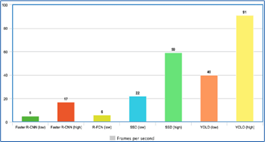
\includegraphics[width=0.4\columnwidth]{bab2/Gambar/Picture29.png}
		\end{center}
		\vspace{-0.2cm}
		%\rule{\columnwidth}{0.1pt}
		\captionsetup{justification=centering}
		\caption{Kecepatan YOLO dibandingkan dengan detector Objek Lainnya\\(Sumber: S. A. S. Hernandez et al, 2020)}\label{img:Kecepatan-YOLO}
	\end{figure}
	%%%%%%%%%%%%%%%%%%%%%%%%%% GAMBAR %%%%%%%%%%%%%%%%%%%%%%%%%%%%%%
	
	\item Akurasi deteksi tinggi (\textit{high detection accuracy})
	
	YOLO jauh melampaui model \textit{state-of-the-art} dalam akurasi dengan sedikit kesalahan latar belakang. 
	
	\item Generalisasi yang bagus (\textit{good generalization})
	
	YOLO mendorong sedikit lebih jauh dengan memberikan generalisasi yang lebih baik untuk domain baru, yang menjadikannya bagus untuk aplikasi yang mengandalkan deteksi objek yang cepat dan kuat. 
	
	\item Sumber terbuka (\textit{open-source})
	
	Membuat YOLO open-source membuat komunitas terus meningkatkan model. Inilah salah satu alasan mengapa YOLO telah melakukan begitu banyak perbaikan dalam waktu yang begitu terbatas. 
	
\end{enumerate}

\subsection{Arsitektur YOLO}
\hspace{1,2cm}Arsitektur YOLO memiliki keseluruhan 24 lapisan konvolusional, empat lapisan penyatuan maksimum, dan dua lapisan yang terhubung sepenuhnya, arsitektur YOLO secara umum pada Gambar \ref{img:Arsitektur-YOLO}.

%%%%%%%%%%%%%%%%%%%%%%%%%% GAMBAR %%%%%%%%%%%%%%%%%%%%%%%%%%%%%%
\begin{figure}[H]
	\vspace{-0.1cm}
	%\rule{\columnwidth}{0.1pt}
	\begin{center}
		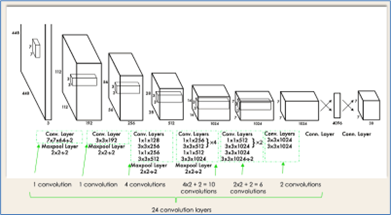
\includegraphics[width=1\columnwidth]{bab2/Gambar/Picture30.png}
	\end{center}
	\vspace{-0.2cm}
	%\rule{\columnwidth}{0.1pt}
	\captionsetup{justification=centering}
	\caption{Arsitektur YOLO dari \textit{Original Paper}\\(J. Redmon et al., 2015)}\label{img:Arsitektur-YOLO}
\end{figure}
%%%%%%%%%%%%%%%%%%%%%%%%%% GAMBAR %%%%%%%%%%%%%%%%%%%%%%%%%%%%%%

Arsitektur YOLO bekerja sebagai berikut: 
\begin{itemize}
	\item Mengubah ukuran gambar input menjadi 448x448 sebelum melalui \textit{convolutional network}. 
	
	\item Konvolusi 1x1 pertama kali diterapkan untuk mengurangi jumlah saluran, yang kemudian diikuti oleh konvolusi 3x3 untuk menghasilkan output kuboid. 
	
	\item Fungsi aktivasi ReLU, kecuali lapisan terakhir, yang menggunakan fungsi aktivasi linier.
	
	\item Beberapa Teknik tambahan, seperti normalisasi batch dan droput, masing-masing mengatur model dan mencegah overfitting. 
\end{itemize}

\subsection{Cara kerja Deteksi Objek YOLO}
\hspace{1,2cm}Berikut ini adalah proses bagaimana YOLO melakukan deteksi objek untuk mendapatkan gambar (b) dari gambar (a) pada Gambar \ref{img:Cara-Kerja-YOLO}.

%%%%%%%%%%%%%%%%%%%%%%%%%% GAMBAR %%%%%%%%%%%%%%%%%%%%%%%%%%%%%%
\begin{figure}[H]
	\vspace{-0.1cm}
	%\rule{\columnwidth}{0.1pt}
	\begin{center}
		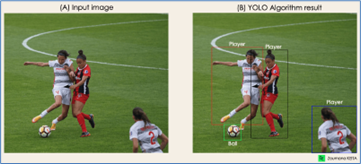
\includegraphics[width=0.9\columnwidth]{bab2/Gambar/Picture31.png}
	\end{center}
	\vspace{-0.2cm}
	%\rule{\columnwidth}{0.1pt}
	\captionsetup{justification=centering}
	\caption{(A) Input Image dan (B) Hasil Algoritma YOLO\\(Sumber: Z. Kelta, 2022)}\label{img:Cara-Kerja-YOLO}
\end{figure}
%%%%%%%%%%%%%%%%%%%%%%%%%% GAMBAR %%%%%%%%%%%%%%%%%%%%%%%%%%%%%%

Algoritma YOLO bekerja berdasarkan empat pendekatan, sebagai berikut:
\begin{enumerate}[label=(\alph*)]
	\item \textit{Residual Blocks}(Blok Sisa)
	
	Langkah pertama dimulai dengan membagi gambar asli (A) menjadi sel grid (NxN) dengan bentuk yang sama, di mana N dalam hal ini adalah 4x4 grid sel pada Gambar \ref{img:Residual-Blocks}. Setiap sel dalam grid bertanggung jawab untuk melokalkan dan memprediksi kelas objek yang dicakupnya, bersama dengan nilai probabilitas/kepercayaan.
	
	%%%%%%%%%%%%%%%%%%%%%%%%%% GAMBAR %%%%%%%%%%%%%%%%%%%%%%%%%%%%%%
	\begin{figure}[H]
		\vspace{-0.1cm}
		%\rule{\columnwidth}{0.1pt}
		\begin{center}
			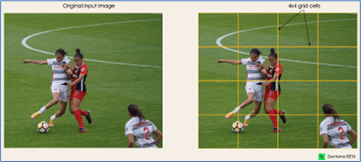
\includegraphics[width=0.9\columnwidth]{bab2/Gambar/Picture32.png}
		\end{center}
		\vspace{-0.2cm}
		%\rule{\columnwidth}{0.1pt}
		\captionsetup{justification=centering}
		\caption{Residual Blocks\\(Sumber: Z. Kelta, 2022)}\label{img:Residual-Blocks}
	\end{figure}
	%%%%%%%%%%%%%%%%%%%%%%%%%% GAMBAR %%%%%%%%%%%%%%%%%%%%%%%%%%%%%%
	
	\item \textit{Bounding Box Regression} (Regresi Kotak Pembatas)
	
	Langkah selanjutnya adalah menentukan kotak pembatas (\textit{bounding box}) yang sesuai dengan persegi Panjang yang menyoroti semua objek dalam gambar. Dapat memiliki kotak pembatas sebanyak objek di dalam gambar yang diberikan. YOLO menentukan atribut kotak pembatas ini menggunakan modul regresi tunggal dalam format berikut, dimana Y adalah representasi vector terakhir untuk setiap kotak pembatas.\\
	Y = [pc, bx, by, bh, bw, c1, c2]\\
	Ini sangat penting selama fase pelatihan model.
	\begin{itemize}
		\item pc sesuai dengan skor probabilitas dari grid yang berisi objek. Misalnya, semua grid yang berwarna merah akan memiliki skor probabilitas lebih tinggi dari nol. Gambar \ref{img:Grid-Probabilitas} adalah versi yang disederhanakan karena probabilitas setiap sel kuning adalah nol (tidak signifikan)
		
		%%%%%%%%%%%%%%%%%%%%%%%%%% GAMBAR %%%%%%%%%%%%%%%%%%%%%%%%%%%%%%
		\begin{figure}[H]
			\vspace{-0.1cm}
			%\rule{\columnwidth}{0.1pt}
			\begin{center}
				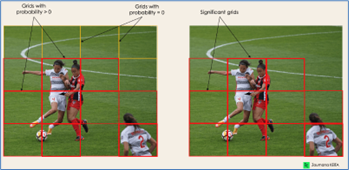
\includegraphics[width=0.9\columnwidth]{bab2/Gambar/Picture33.png}
			\end{center}
			\vspace{-0.2cm}
			%\rule{\columnwidth}{0.1pt}
			\captionsetup{justification=centering}
			\caption{Grid dengan Probabilitas\\(Sumber: Z. Kelta, 2022)}\label{img:Grid-Probabilitas}
		\end{figure}
		%%%%%%%%%%%%%%%%%%%%%%%%%% GAMBAR %%%%%%%%%%%%%%%%%%%%%%%%%%%%%%
		
		\item bx dan by adalah koordinat x dan y dari pusat kotak pembatas (\textit{center of bounding box}) sehubungan dengan grid sel pembungkus. 
		
		\item bh dan bw sesuai dengan tinggi dan lebar kotak pembatas sehubungan dengan sel grid pembungkus
		
		\item c1 dan c2 sesuai dengan dua kelas Player dan Ball, dapat memiliki kelas sebanyak yang dibutuhkan oleh pengguna.
		
		Untuk dapat memahami dan terlihat, seperti pada Gambar \ref{img:Cara-Bounding-Box} berikut.
		%%%%%%%%%%%%%%%%%%%%%%%%%% GAMBAR %%%%%%%%%%%%%%%%%%%%%%%%%%%%%%
		\begin{figure}[H]
			\vspace{-0.1cm}
			%\rule{\columnwidth}{0.1pt}
			\begin{center}
				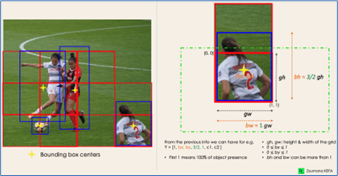
\includegraphics[width=0.9\columnwidth]{bab2/Gambar/Picture34.png}
			\end{center}
			\vspace{-0.2cm}
			%\rule{\columnwidth}{0.1pt}
			\captionsetup{justification=centering}
			\caption{Cara \textit{Bounding Box}\\(Sumber: Z. Kelta, 2022)}\label{img:Cara-Bounding-Box}
		\end{figure}
		%%%%%%%%%%%%%%%%%%%%%%%%%% GAMBAR %%%%%%%%%%%%%%%%%%%%%%%%%%%%%%
	\end{itemize}
	
	\item \textit{Intersection Over Unions} (IOU)
	
	Sebagian besar waktu, satu objek dalam gambar dapat memiliki beberapa kandidat kotak petak untuk prediksi, meskipun tidak semuanya relevan. Tujuan dari IOU (nilai antara 0 dan 1) adalah untuk membuang kotak kisi tersebut agar hanya menyimpan yang relevan. Inilah logika dari IOU:
	
	\begin{itemize}
		\item Pengguna menentukan ambang pemilihan IOU-nya, misalnya, 0,5.
		
		\item Kemudian YOLO menghitung IOU dari setiap sel grid yang merupakan area persimpangan dibagi dengan Union Area.
		
		\item Terakhir, ia mengabaikan prediksi sel kisi yang memiliki IOU $\leq$ ambang batas dan mempertimbangkannya dengan IOU > ambang batas.
	\end{itemize}
	
	Pada Gambar \ref{img:IOU} adalah ilustrasi penerapan proses pemilihan grid pada objek kiri bawah. Dapat diamati bahwa objek awalnya memiliki dua kandidat kisi, kemudian hanya "Kisi 2" yang dipilih di bagian akhir.
	
	%%%%%%%%%%%%%%%%%%%%%%%%%% GAMBAR %%%%%%%%%%%%%%%%%%%%%%%%%%%%%%
	\begin{figure}[H]
		\vspace{-0.1cm}
		%\rule{\columnwidth}{0.1pt}
		\begin{center}
			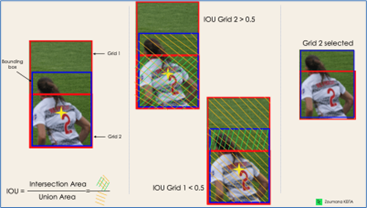
\includegraphics[width=0.9\columnwidth]{bab2/Gambar/Picture35.png}
		\end{center}
		\vspace{-0.2cm}
		%\rule{\columnwidth}{0.1pt}
		\captionsetup{justification=centering}
		\caption{IOU\\(Sumber: Z. Kelta, 2022)}\label{img:IOU}
	\end{figure}
	%%%%%%%%%%%%%%%%%%%%%%%%%% GAMBAR %%%%%%%%%%%%%%%%%%%%%%%%%%%%%%
	
	\item Non-Maximum Supression (NMS)
	
	Menetapkan ambang batas untuk IOU tidak selalu cukup karena sebuah objek dapat memiliki beberapa kotak dengan IOU di luar ambang batas, dan meninggalkan semua kotak tersebut mungkin termasuk kebisingann (\textit{noise}). Di sinilah, dapat menggunakan NMS untuk menyimpan hanya kotak dengan skor probabilitas deteksi tertinggi.
\end{enumerate}

\subsection{Perkembangan YOLO}
\hspace{1,2cm}Sejak rilis pertama YOLO pada tahun 2015, YOLO telah banyak berkembang dengan versi berbeda, seperti pada Gambar \ref{img:Perkembangan-YOLO}. 

%%%%%%%%%%%%%%%%%%%%%%%%%% GAMBAR %%%%%%%%%%%%%%%%%%%%%%%%%%%%%%
\begin{figure}[H]
	\vspace{-0.1cm}
	%\rule{\columnwidth}{0.1pt}
	\begin{center}
		\includegraphics[width=0.9\columnwidth]{bab2/Gambar/Picture36.png}
	\end{center}
	\vspace{-0.2cm}
	%\rule{\columnwidth}{0.1pt}
	\captionsetup{justification=centering}
	\caption{Perkembangan YOLO\\(Sumber: Z. Kelta, 2022)}\label{img:Perkembangan-YOLO}
\end{figure}
%%%%%%%%%%%%%%%%%%%%%%%%%% GAMBAR %%%%%%%%%%%%%%%%%%%%%%%%%%%%%%

\begin{enumerate}
	\item YOLO atau YOLOv1
	
	Versi pertama YOLO ini adalah pengubah permainan untuk deteksi objek, karena kemampuannya mengenali objek dengan cepat dan efisien.\\
	Namun, seperti banyak solusi lainnya, versi pertama YOLO memiliki keterbatasannya sendiri:
	\begin{itemize}
		\item Kesulitan untuk mendeteksi gambar yang lebih kecil dalam sekelompok gambar, seperti sekelompok orang di stadion. Ini karena setiap kisi dalam arsitektur YOLO dirancang untuk deteksi objek tunggal.
		
		\item Kemudian, YOLO tidak berhasil mendeteksi bentuk baru atau tidak biasa.
		
		\item Terakhir, fungsi kerugian yang digunakan untuk memperkirakan kinerja pendeteksian memperlakukan kesalahan yang sama untuk kotak pembatas kecil dan besar, yang sebenarnya membuat pelokalan yang salah.
	\end{itemize}
	
	\item YOLOv2 atau YOLO9000
	
	YOLOv2 dibuat pada tahun 2016 dengan ide membuat model YOLO lebih baik, lebih cepat, dan lebih kuat.\\
	Peningkatan termasuk tetapi tidak terbatas pada penggunaan Darknet-19 sebagai arsitektur baru, normalisasi batch, resolusi input yang lebih tinggi, lapisan konvolusi dengan anchors, pengelompokan dimensi, dan (5) fitur-fitur halus.
	
	\begin{itemize}
		\item \textit{Batch Normalization}
		
		Menambahkan lapisan normalisasi batch meningkatkan kinerja sebesar 2\% mAP. Normalisasi batch ini menyertakan efek regularisasi, mencegah overfitting.
		
		\item \textit{Higher input resolution}
		
		YOLOv2 secara langsung menggunakan input 448x448 beresolusi lebih tinggi daripada 224x224, yang membuat model menyesuaikan filternya untuk bekerja lebih baik pada gambar beresolusi lebih tinggi. Pendekatan ini meningkatkan akurasi sebesar 4\% mAP, setelah dilatih selama 10 epochs pada data ImageNet.
	\end{itemize}
	
	\item YOLOv3 - Peningkatan Bertahap
	
	Perubahan tersebut terutama mencakup arsitektur jaringan baru: Darknet-53. Ini adalah jaringan saraf 106, dengan jaringan upsampling dan blok residual. Jauh lebih besar, lebih cepat, dan lebih akurat dibandingkan dengan Darknet-19, yang merupakan tulang punggung YOLOv2. Arsitektur baru ini telah bermanfaat di banyak tingkatan:
	
	\begin{itemize}
		\item Prediksi \textit{Bounding Box} Lebih Baik
		
		Model regresi logistic digunakan oleh YOLOv3 untuk memprediksi skor objektivitas untuk setiap kotak pembatas (bounding box).
		
		\item Prediksi Kelas yang Lebih Akurat
		
		Menggantikan penggunaan softmax seperti yang dilakukan di YOLOv2, pengklasifikasi logistik independen telah diperkenalkan untuk memprediksi kelas kotak pembatas secara akurat. Ini bahkan berguna saat menghadapi domain yang lebih kompleks dengan label yang tumpang tindih (Misalnya, $\rightarrow$ Pemain Sepak Bola). Menggunakan softmax akan membatasi setiap kotak hanya memiliki satu kelas, yang tidak selalu benar.
		
	\end{itemize}
	
	\item YOLOv4 - \textit{Optimal Speed dan Accuracy of Object Detection}
	
	Versi YOLO ini memiliki Kecepatan dan Akurasi Deteksi Objek Optimal dibandingkan dengan semua versi sebelumnya dan detektor objek canggih lainnya.\\
	Gambar \ref{img:KomprasiYoloV4-YoloV3} menunjukkan YOLOv4 mengungguli YOLOv3 dan FPS dalam kecepatan masing-masing sebesar 10\% dan 12\%.
	
	%%%%%%%%%%%%%%%%%%%%%%%%%% GAMBAR %%%%%%%%%%%%%%%%%%%%%%%%%%%%%%
	\begin{figure}[H]
		\vspace{-0.1cm}
		%\rule{\columnwidth}{0.1pt}
		\begin{center}
			\includegraphics[width=0.8\columnwidth]{bab2/Gambar/Picture37.png}
		\end{center}
		\vspace{-0.2cm}
		%\rule{\columnwidth}{0.1pt}
		\captionsetup{justification=centering}
		\caption{Komparasi YOLOv4 dengan YOLOv3 dan \textit{state-of-the-art} Deteksi Objek Lain \\(Sumber: Z. Kelta, 2022)}\label{img:KomprasiYoloV4-YoloV3}
	\end{figure}
	%%%%%%%%%%%%%%%%%%%%%%%%%% GAMBAR %%%%%%%%%%%%%%%%%%%%%%%%%%%%%%
	YOLOv4 dirancang khusus untuk sistem produksi dan dioptimalkan untuk komputasi paralel.\\
	\textit{Backbone} arsitektur YOLOv4 adalah CSPDarknet53, jaringan yang berisi 29 lapisan konvolusi dengan filter 3 x 3 dan sekitar 27,6 juta parameter.\\
	Arsitektur ini, dibandingkan dengan YOLOv3, menambahkan informasi berikut untuk deteksi objek yang lebih baik:
	
	\begin{itemize}
		\item \textit{Spatial Pyramid Pooling} (SPP) secara signifikan meningkatkan bidang reseptif, memisahkan fitur konteks yang paling relevan, dan tidak memengaruhi kecepatan jaringan.
		
		\item Menggantikan \textit{Feature Pyramid Network} (FPN) yang digunakan di YOLOv3, YOLOv4 menggunakan PANet untuk agregasi parameter dari tingkat deteksi yang berbeda.
		
		\item Augmentasi data menggunakan teknik mosaik yang menggabungkan empat gambar pelatihan selain pendekatan pelatihan permusuhan diri.
		
		\item Menggunakan pemilihan hyper-parameter yang optimal menggunakan algoritma genetika.
		
	\end{itemize}
	
	\item YOLOR - You Only Look One Representation
	
	Sebagai \textit{Unified Network for Multiple Tasks}, YOLOR didasarkan pada jaringan terpadu yang merupakan kombinasi dari pendekatan pengetahuan eksplisit dan implisit.
	
	%%%%%%%%%%%%%%%%%%%%%%%%%% GAMBAR %%%%%%%%%%%%%%%%%%%%%%%%%%%%%%
	\begin{figure}[H]
		\vspace{-0.1cm}
		%\rule{\columnwidth}{0.1pt}
		\begin{center}
			\includegraphics[width=0.8\columnwidth]{bab2/Gambar/Picture38.png}
		\end{center}
		\vspace{-0.2cm}
		%\rule{\columnwidth}{0.1pt}
		\captionsetup{justification=centering}
		\caption{Unified Network Architecture\\(Sumber: C. Y. Wang et al, 2021}\label{img:Unified-Network-Architecture}
	\end{figure}
	%%%%%%%%%%%%%%%%%%%%%%%%%% GAMBAR %%%%%%%%%%%%%%%%%%%%%%%%%%%%%%
		Pengetahuan eksplisit adalah pembelajaran normal atau conscious learning. Pembelajaran implisit di sisi lain dilakukan secara tidak sadar (dari pengalaman).\\
		Menggabungkan kedua teknik ini, YOLOR mampu menciptakan arsitektur yang lebih kuat berdasarkan tiga proses: (1) penyelarasan fitur, (2) penyelarasan prediksi untuk deteksi objek, dan (3) representasi kanonis untuk pembelajaran multi-tugas.\\
		Salah satu yang mengalami peningkatan adalah penjajaran prediksi. Pendekatan ini memperkenalkan representasi implisit ke dalam peta fitur dari setiap jaringan piramida fitur (FPN), yang meningkatkan presisi sekitar 0,5\%.\\
		Dari grafik berikut, dapat diamati bahwa YOLOR mencapai kecepatan inferensi data MS COCO yang canggih dibandingkan dengan model lain seperti pada Gambar \ref{img:Performance-YOLOR-YOLOV4}.
		
	%%%%%%%%%%%%%%%%%%%%%%%%%% GAMBAR %%%%%%%%%%%%%%%%%%%%%%%%%%%%%%
	\begin{figure}[H]
		\vspace{-0.1cm}
		%\rule{\columnwidth}{0.1pt}
		\begin{center}
			\includegraphics[width=0.8\columnwidth]{bab2/Gambar/Picture39.png}
		\end{center}
		\vspace{-0.2cm}
		%\rule{\columnwidth}{0.1pt}
		\captionsetup{justification=centering}
		\caption{Performance YOLOR vs YOLOv4 dan Model Lainnya\\(Sumber: C. Y. Wang et al, 2021}\label{img:Performance-YOLOR-YOLOV4}
	\end{figure}
	%%%%%%%%%%%%%%%%%%%%%%%%%% GAMBAR %%%%%%%%%%%%%%%%%%%%%%%%%%%%%%
	
	\item YOLOX - Exciding \textit{YOLO Series in 2021}
	
	Ini menggunakan baseline yang merupakan versi modifikasi dari YOLOv3, dengan Darknet-53 sebagai \textit{backbone}.\\
	Diterbitkan dalam makalah \textit{Exceeding} YOLO \textit{Series in 2021}, YOLOX menghadirkan empat karakteristik utama berikut untuk membuat model yang lebih baik dibandingkan dengan versi yang lebih lama.
	
	\begin{itemize}
		\item Kepala terpisah yang efisien: Coupled head yang digunakan pada versi YOLO sebelumnya terbukti mengurangi performa model. YOLOX menggunakan decoupled sebagai gantinya, yang memungkinkan pemisahan tugas klasifikasi dan lokalisasi, sehingga meningkatkan kinerja model.
		
		\item Augmentasi data yang kuat: Integrasi Mosaic dan MixUp ke dalam pendekatan augmentasi data sangat meningkatkan kinerja YOLOX.
		
		\item \textit{Anchor free system}: Algoritma \textit{anchor-based} melakukan pengelompokan di bawah tenda, yang meningkatkan waktu inferensi. Menghapus mekanisme jangkar di YOLOX mengurangi jumlah prediksi per gambar, dan meningkatkan waktu inferensi secara signifikan.
		
		\item SimOTA untuk penetapan label: Pergantian penggunaan pendekatan interseksi penyatuan (IoU), penulis memperkenalkan SimOTA, strategi penetapan label yang lebih kuat yang mencapai hasil canggih dengan tidak hanya mengurangi waktu pelatihan tetapi juga menghindari masalah hiperparameter tambahan. Selain itu, ini meningkatkan peta deteksi sebesar 3\%.
		
	\end{itemize}
	
	\item YOLOv5
	
	YOLOv5, dibandingkan dengan versi lain, tidak memiliki makalah penelitian yang diterbitkan, dan ini adalah versi YOLO pertama yang diimplementasikan di Pytorch, bukan di Darknet.\\
	Dirilis oleh Glenn Jocher pada Juni 2020, YOLOv5, mirip dengan YOLOv4, menggunakan CSPDarknet53 sebagai tulang punggung arsitekturnya. Rilis ini mencakup lima ukuran model yang berbeda: YOLOv5s (terkecil), YOLOv5m, YOLOv5l, dan YOLOv5x (terbesar).\\
	Salah satu peningkatan besar dalam arsitektur YOLOv5 adalah integrasi lapisan Fokus, yang diwakili oleh satu lapisan, yang dibuat dengan mengganti tiga lapisan pertama YOLOv3. Integrasi ini mengurangi jumlah lapisan, dan jumlah parameter dan juga meningkatkan kecepatan maju dan mundur tanpa dampak besar pada peta.\\
	Ilustrasi Gambar \ref{img:Perbandingan-YOLOv4-YOLOv5} membandingkan waktu pelatihan antara YOLOv4 dan YOLOv5.
	
	%%%%%%%%%%%%%%%%%%%%%%%%%% GAMBAR %%%%%%%%%%%%%%%%%%%%%%%%%%%%%%
	\begin{figure}[H]
		\vspace{-0.1cm}
		%\rule{\columnwidth}{0.1pt}
		\begin{center}
			\includegraphics[width=0.6\columnwidth]{bab2/Gambar/Picture40.png}
		\end{center}
		\vspace{-0.2cm}
		%\rule{\columnwidth}{0.1pt}
		\captionsetup{justification=centering}
		\caption{Perbandingan Waktu Pelatihan antara YOLOv4 dan YOLOv5\\(Sumber: J. Nelson, 2020}\label{img:Perbandingan-YOLOv4-YOLOv5}
	\end{figure}
	%%%%%%%%%%%%%%%%%%%%%%%%%% GAMBAR %%%%%%%%%%%%%%%%%%%%%%%%%%%%%%
	
	\item YOLOv6
	
	Didedikasikan untuk aplikasi industri dengan desain efisien yang ramah perangkat keras dan kinerja tinggi, kerangka kerja YOLOv6 (MT-YOLOv6) dirilis oleh Meituan, sebuah perusahaan e-commerce Tiongkok.\\
	Ditulis dalam Pytorch, versi baru ini bukan bagian dari YOLO resmi tetapi tetap diberi nama YOLOv6 karena tulang punggungnya terinspirasi oleh arsitektur YOLO satu tahap yang asli.\\
	YOLOv6 memperkenalkan tiga peningkatan signifikan pada YOLOv5 sebelumnya: desain tulang punggung dan leher yang ramah perangkat keras, kepala terpisah yang efisien, dan strategi pelatihan yang lebih efektif.\\
	YOLOv6 memberikan hasil yang luar biasa dibandingkan dengan versi YOLO sebelumnya dalam hal akurasi dan kecepatan pada dataset COCO seperti yang diilustrasikan pada Gambar \ref{img:Performance-YOLOv6}
	
	%%%%%%%%%%%%%%%%%%%%%%%%%% GAMBAR %%%%%%%%%%%%%%%%%%%%%%%%%%%%%%
	\begin{figure}[H]
		\vspace{-0.1cm}
		%\rule{\columnwidth}{0.1pt}
		\begin{center}
			\includegraphics[width=1\columnwidth]{bab2/Gambar/Picture41.png}
		\end{center}
		\vspace{-0.2cm}
		%\rule{\columnwidth}{0.1pt}
		\captionsetup{justification=centering}
		\caption{Comparison of state-of-the-art efficient object detectors. All models are tested with TensorRT 7 except that the quantized model is with TensorRT 8\\(Sumber: C. Li et al, 2022}\label{img:Performance-YOLOv6}
	\end{figure}
	%%%%%%%%%%%%%%%%%%%%%%%%%% GAMBAR %%%%%%%%%%%%%%%%%%%%%%%%%%%%%%
	
	\begin{itemize}
		\item YOLOv6-N mencapai 35,9\% AP pada dataset COCO dengan throughput 1234 (throughput) FPS pada GPU NVIDIA Tesla T4.
		
		\item YOLOv6-S mencapai AP 43,3\% yang canggih pada 869 FPS.
		
		\item YOLOv6-M dan YOLOv6-L juga mencapai kinerja akurasi yang lebih baik masing-masing sebesar 49,5\% dan 52,3\% dengan kecepatan inferensi yang sama.
		
	\end{itemize}
	
	\item YOLOv7
	
	YOLOv7 dirilis pada Juli 2022 di Paper \textit{Trained bag-of-freebies set state-of-the-art real-time object detector}. Versi ini membuat langkah signifikan di bidang deteksi objek, dan melampaui semua model sebelumnya dalam hal akurasi dan kecepatan.
	
	%%%%%%%%%%%%%%%%%%%%%%%%%% GAMBAR %%%%%%%%%%%%%%%%%%%%%%%%%%%%%%
	\begin{figure}[H]
		\vspace{-0.1cm}
		%\rule{\columnwidth}{0.1pt}
		\begin{center}
			\includegraphics[width=1\columnwidth]{bab2/Gambar/Picture42.png}
		\end{center}
		\vspace{-0.2cm}
		%\rule{\columnwidth}{0.1pt}
		\captionsetup{justification=centering}
		\caption{Perbandingan YOLOv7 inference time dengan real-time object detector lainnya\\(Sumber: C. Y. Wang et al, 2022}\label{img:Performance-YOLOv7}
	\end{figure}
	%%%%%%%%%%%%%%%%%%%%%%%%%% GAMBAR %%%%%%%%%%%%%%%%%%%%%%%%%%%%%%
	YOLOv7 telah membuat perubahan besar dalam (1) arsitekturnya dan (2) pada tingkat bag-of-freebies yang dapat dilatih:
	
	\begin{itemize}
		\item Level Aristektur
		
		YOLOv7 mereformasi arsitekturnya dengan mengintegrasikan Extended Efficient Layer Aggregation Network (E-ELAN) yang memungkinkan model mempelajari fitur yang lebih beragam untuk pembelajaran yang lebih baik.\\
		Selain itu, YOLOv7 menskalakan arsitekturnya dengan menggabungkan arsitektur model asalnya seperti YOLOv4, Scaled YOLOv4, dan YOLO-R. Hal ini memungkinkan model untuk memenuhi kebutuhan kecepatan inferensi yang berbeda.
		
		%%%%%%%%%%%%%%%%%%%%%%%%%% GAMBAR %%%%%%%%%%%%%%%%%%%%%%%%%%%%%%
		\begin{figure}[H]
			\vspace{-0.1cm}
			%\rule{\columnwidth}{0.1pt}
			\begin{center}
				\includegraphics[width=1\columnwidth]{bab2/Gambar/Picture43.png}
			\end{center}
			\vspace{-0.2cm}
			%\rule{\columnwidth}{0.1pt}
			\captionsetup{justification=centering}
			\caption{\textit{Compound scaling up depth and width for concatenation-based model}\\(Sumber: C. Y. Wang et al, 2022}\label{img:Compund-Scaling}
		\end{figure}
		%%%%%%%%%%%%%%%%%%%%%%%%%% GAMBAR %%%%%%%%%%%%%%%%%%%%%%%%%%%%%%
		
		\item Trainable bag-of-freebies
		
		Istilah bag-of-freebies mengacu pada peningkatan akurasi model tanpa meningkatkan biaya pelatihan, dan inilah alasan mengapa YOLOv7 tidak hanya meningkatkan kecepatan inferensi tetapi juga akurasi deteksi.
		
	\end{itemize}
\end{enumerate}

\section{Object Based Image Analysis (OBIA)}
\hspace{1,2cm}OBIA merupakan teknik klasifikasi yang tidak hanya memandang rona dan tekstur piksel namun berdasarkan dari kesatuan objek, atau dapat dikatakan OBIA adalah pendekatan yang proses klasifikasinya tidak hanya mempertimbangkan aspek spectral naum aspek spasial objek. Data citra penginderaan jauh yang digunakan untuk klasifikasi ini biasanya menggunakan data citra penginderaan jauh resolusi tinggi seperti QUickbird, Ikonos, World View, dll. Klasifikasi ini hamper mirip dengan klasifikasi unsupervised, akan tetapi basis dari klasifikasi OBIA yaitu dengan segmentasi (A. Bakar, 2014).

OBIA mengelompokkan gambar yang mengelompokkan piksel kecil menjadi objek vektor. Alih-alih berbasis per-pixel, segmentasi secara otomatis mendigitalkan gambar untuk pengguna (GIS Geography, 2020).

%%%%%%%%%%%%%%%%%%%%%%%%%% GAMBAR %%%%%%%%%%%%%%%%%%%%%%%%%%%%%%
\begin{figure}[H]
	\vspace{-0.1cm}
	%\rule{\columnwidth}{0.1pt}
	\begin{center}
		\includegraphics[width=1\columnwidth]{bab2/Gambar/Picture44.png}
	\end{center}
	\vspace{-0.2cm}
	%\rule{\columnwidth}{0.1pt}
	\captionsetup{justification=centering}
	\caption{OBIA Segmentasi Proses Pengelompokkkan Pixel yang hampir sama ke dalam Objek\\(Sumber: GISGeography, 2020)}\label{img:OBIA-Segmentasi-Proses}
\end{figure}
%%%%%%%%%%%%%%%%%%%%%%%%%% GAMBAR %%%%%%%%%%%%%%%%%%%%%%%%%%%%%%

Apa yang dilakukan segmentasi adalah meniru apa yang dilakukan mata pengguna. Tetapi dengan objek tersegmentasi ini, pengguna menggunakan properti spektral, geometris, dan spasialnya untuk mengklasifikasikan ke dalam tutupan lahan.

%%%%%%%%%%%%%%%%%%%%%%%%%% GAMBAR %%%%%%%%%%%%%%%%%%%%%%%%%%%%%%
\begin{figure}[H]
	\vspace{-0.1cm}
	%\rule{\columnwidth}{0.1pt}
	\begin{center}
		\includegraphics[width=1\columnwidth]{bab2/Gambar/Picture45.png}
	\end{center}
	\vspace{-0.2cm}
	%\rule{\columnwidth}{0.1pt}
	\captionsetup{justification=centering}
	\caption{OBIA Klasifikasi menggunakan shape, size, dan spectral properties objek untuk klasifikasi setiap objek}\label{img:OBIA-Klasifikasi}
\end{figure}
%%%%%%%%%%%%%%%%%%%%%%%%%% GAMBAR %%%%%%%%%%%%%%%%%%%%%%%%%%%%%%

Dua prinsip dasar OBIA adalah klasifikasi dan segmentasi. Segmentasi adalah memecah gambar menjadi objek yang mewakili fitur berbasis darat, sedangkan Klasifikasi adalah mengklasifikasi objek-objek tersebut menggunakan bentuk, ukuran, sifat spasial dan spektralnya. Analis sering menggunakan statistik ini untuk mengklasifikasikan tutupan lahan menggunakan OBIA, yaitu \textit{trees} (pohon) memiliki ketinggian yang bervariasi (standar deviasi \textit{normalized Digital Surface Model} (nDSM)) yang merupakan model elevasi yang menangkap fitur alami dan fitur buatan, seperti gedung, pohon, kabel listrik, dan objek lainnya. Di samping itu, memiliki reflektansi inframerah-dekat yang tinggi (\textit{normalized difference vegetation index} (NDVI) tinggi), sedangkan \textit{grass} memiliki pendek (nDSM rendah), datar (deviasi standar nDSM rendah) dan memiliki reflektansi inframerah-dekat sedang (NDVI sedang). NDVI digunakan untuk mengukur indeks yang menggambarkan tingkat kepadatan, kehijauan suatu tanaman dan kondisi dari suatu vegetasi.

\section{Sentinel-2}
\hspace{1,2cm}Data yang digunakan dalam penelitian ini diambil dari gambar citra satelit Sentinel-2. Sentinel-2 diluncurkan sebagai bagian dari program Copernicus Komisi Eropa pada tanggal 23 Juni 2015 yang dirancang khusus untuk memberikan banyak data dan citra. Satelit dilengkapi dengan sensor multispectral opto-elektronik untuk survei dengan resoulsi Sentinel-2 yaitu 10 hingga 60m di zona spekatral tampak, VNIR, SWIR, termasuk 13 saluran spectral yang memastikan penangkapan perbedaan dalam keadaan vegetasi, termasuk perubahan temporal, dna juga meminimalkan dampkan kualitas fotografi atmosfer. Sentinel-2 memiliki dua satelit dalam misi memungkinkan survei berulang setiap 5 hari di ekuator dan 2-3 hari di garis lintang tengah (EOS, 2020). 

Misi Sentinel-2 terdiri dari dua satelit yang dikembangkan untuk mendukung vegetasi, tutupan lahan, dan pemantauan lingkungan. Satelit Sentinel-2A diluncurkan oleh European Space Agency (ESA) pada 23 Juni 2015, dan beroperasi di orbit sinkron matahari dengan siklus berulang 10 hari. Setelit kedua yaitu Sentinel-2B diluncurkan pada 7 Maret 2017 dan beroperasi dengan akuisisi data yang tersedia di EarthExplorer (USGS EROS, 2020). 

Terdapat Perbandingan antara Sentinel-2 dengan UAV Drone, seperti pada Tabel 2.2.

%%% BENERIN TABEL

\section{Pertanian Presisi}
\hspace{1,2cm}Pertanian presisi atau precision agriculture merupakan suatu sistem pertanian yang mengintegrasikan penggunaan teknologi dalam mengumpulkan informasi, sehingga dapat melakukan proses pertanian secara presisi atau dengan input, tempat, dan waktu yang tepat. Istilah presisi berarti akurat, terakar, dan terukur. Pertanian presisi disebut juga menggunakan input pertanian yang tepat dengan teknik, jumlah, tempat, dan waktu yang tepat untuk menghasilkan produksi panen secara maksimal. Input pertanian meliputi seperti pemupukan, herbisida, insektisida, benih, dan lainnya. Meskipun untuk melakukan pertanian secara akurat ini membutuhkan banyak informasi, cenderung kompleks untuk kebanyakan petani, dan membutuhkan kerjasama dari berbagai multidisiplin ilmu, namun sistem pertanian presisi mampu meingkatkan laba, mengurangi limbah, mengurangi biaya produksi, dan menjaga kualitas lingkungan (J. Taylor et al., 2016). 

Pertanian presisi (PA) merupakan ilmu untuk meningkatkan hasil panen dan membantu keputusan manajemen menggunakan sensor dan alat analisis teknologi tinggi. Pertanian presisi adalah konsep yang digunakan untuk meningkatkan produksi, mengurangi waktu kerja, dan memastikan pengelolaan seperti pupuk, irigasi, dan lainnya berjalan efektif. Perkembangan teknologi, khususnya ketersediaan citra satelit beresolusi tinggi, perkembangan teknologi kendaraan udara tak berawak (UAV), menunjukkan bahwa adopsi sumber data penginderaan jauh dalam pertanian presisi mengalami peningkatan (P. Singh et al., 2020). 

Siklus pertanian presisi terdiri dari tahapan seperti Gambar 2.46.
%%%%%%%%%%%%%%%%%%%%%%%%%% GAMBAR %%%%%%%%%%%%%%%%%%%%%%%%%%%%%%
\begin{figure}[H]
	\vspace{-0.1cm}
	%\rule{\columnwidth}{0.1pt}
	\begin{center}
		\includegraphics[width=1\columnwidth]{bab2/Gambar/Picture46.png}
	\end{center}
	\vspace{-0.2cm}
	%\rule{\columnwidth}{0.1pt}
	\captionsetup{justification=centering}
	\caption{Siklus Pertanian Presisi\\(Sumber: A. Comparetti, 2011)}\label{img:Siklus-Pertanian-Presisi}
\end{figure}
%%%%%%%%%%%%%%%%%%%%%%%%%% GAMBAR %%%%%%%%%%%%%%%%%%%%%%%%%%%%%%
\begin{itemize}
	\item Pengukuran parameter tanah dan tanaman dengan bantuan pemetaan spasial dan pemantauan kondisi cuaca setempat (pengumpulan data);
	
	\item pemetaan parameter tanah dan tanaman dalam lapangan (pengumpulan data);
	
	\item pemetaan dan integrasi data dengan bantuan aplikasi (interpretasi);
	
	\item pemantauan kesuburan dan penaburan (aplikasi);
	
\end{itemize}
Dalam menerapkan pertanian presisi diperlukan instrumen berikut (A. Comparetti, 2011):

\begin{itemize}
	\item Sistem penentuan posisi satelit, untuk penginderaan posisi di mana setiap parameter lapangan yang diukur harus direferensikan secara geografis dan, kemudian, juga posisi di mana input (seperti, tanaman, lahan) yang terdeteksi oleh  mesin dapat diterapkan kebutuhannya di setiap area lahan (zona pengelolaan).
	
	\item Sensor, untuk mengukur parameter tanah dan tanaman di lapangan.
	
	\item Perangkat (devices), untuk menyiapkan dan mengontrol aplikasi input tanaman tingkat variabel spasial.
	
	\item Perangkat lunak, untuk membuat peta parameter tanah dan tanaman dalam lahan dan aplikasi input tanaman dengan data dari citra penginderaan, dan juga untuk menginterpretasikan data terukur;
	
\end{itemize}

\section{Kelapa Sawit}
\hspace{1,2cm}Kelapa sawit adalah tanaman sejenis palma berakar serabut atau monokotil. Bagian tanaman yang bernilai ekonomis adalah buah. Masing-masing dari seribu atau lebih buah dalam tandan buah segar itu terdiri dari inti sawit (kernel) yang dikelilingi) oleh daging buah (mesocarp). Di pabrik kelapa sawit, sangat sedikit buah yang terbuang sia-sia karena pabrik tersebut mengubah setiap buah kelapa sawit menjadi minyak kelapa sawit dan minyak inti sawit), bahkan limbah dari setiap buah sawitpun di daur ulang di perkebunan sebagai pupuk atau diolah sebagai bahan bakar biomass. Sangat sedikit sekali buah kelapa sawit terbuang karena baik inti kelapa sawit dan dagingnya sama-sama digunakan untuk menghasilkan minyak.

%%%%%%%%%%%%%%%%%%%%%%%%%% GAMBAR %%%%%%%%%%%%%%%%%%%%%%%%%%%%%%
\begin{figure}[H]
	\vspace{-0.1cm}
	%\rule{\columnwidth}{0.1pt}
	\begin{center}
		\includegraphics[width=0.3\columnwidth]{bab2/Gambar/Picture47.jpg}
	\end{center}
	\vspace{-0.2cm}
	%\rule{\columnwidth}{0.1pt}
	\captionsetup{justification=centering}
	\caption{Buah Kelapa Sawit(Inti dan Daging Sawit)}\label{img:Buah-Kelapa-Sawit}
\end{figure}
%%%%%%%%%%%%%%%%%%%%%%%%%% GAMBAR %%%%%%%%%%%%%%%%%%%%%%%%%%%%%%

Satu tandan tanaman dewasa beratnya mencapai 20 - 35 kg, bahkan ada yang mencapai di atas 40 kg, tergantung pada perawatan. Tandan tersusun dari 200 - 600 buah masing-masing sekitar 20-35 gram. Buah diambil minyaknya dengan hasil sabut (daging buah/mesocarp) menghasilkan minyak kasar (CPO) 20-26\%, inti sawit sebanyak 6\% yang menghasilkan minyak inti (PKO) 3-4\%. Kadar \% dihitung dari berat tandan buah segar (Smart Agribusiness and Food, 2017).

\begin{enumerate}[label=(\alph*)]
	\item Usia Tanam
	
	Umur atau usia ekonomis tanaman kelapa sawit yang dibudidayakan bisa mencapai usia hingga 25 tahun. Pada usia tanam sudah tinggi, sehingga sulit dipanen, tandanya sudah jarang sehingga secara perhitungan tidak ekonomis lagi. Pengelompokkan berdasarkan masa berbuah (PTPN, 2018), seperti Tabel \ref{tbl:Pengelompokkan-Berdasarkan-Masa-Berubah} berikut ini:
	
	%%%%%%%%%%%%%%%%%%%%%%%TABEL SEDERHANA%%%%%%%%%%%%%%%%%%%%%%%%%
	\begin{singlespace}
		\begin{table}[H]
			\centering
			\caption{Pengelompokkan Berdasarkan Masa Berbuah}
			\label{tbl:Pengelompokkan-Berdasarkan-Masa-Berubah}
			\begin{tabular}{|p{6cm}|p{6cm}|}
				\hline
				\multicolumn{1}{|c|}{Kelompok}   & Masa Berbuah (Tahun) \\ \hline
				Tanaman Belum Menghasilkan (TBM) & 0-3                  \\ \hline
				Tanaman Menghasilkan             & \textgreater{}3      \\ \hline
			\end{tabular}
		\end{table}
	\end{singlespace}
	%%%%%%%%%%%%%%%%%%%%%%%TABEL SEDERHANA%%%%%%%%%%%%%%%%%%%%%%%%%
	
	\item Produktivitas Tanaman Kelapa Sawit Menurut Umur Tanaman
	
	Produktivitas tanaman kelapa sawit (tandan buah segar (TBS)) menurut umur tanaman dalam Kondisi Kebun Percobaan Balit Marihat berdasarkan PTPN. VII tahun 1993 dalam \textit{lecture note} "Budi Daya Kelapa Sawit" (S. Yahya \& Suwarto, 2021), seperti Tabel 2.4. berikut ini:
	
	%%%%%%%%%%%%%%%%%%%%%%%TABEL SEDERHANA%%%%%%%%%%%%%%%%%%%%%%%%%
	\begin{singlespace}
		\begin{table}[H]
			\centering
			\caption{Produktivitas Tanaman Kelapa Sawit Menurut Umur Tanaman dalam Kondisi Kebun Percobaan Balit Marihat}
			\label{tbl:Produktivitas-Tanaman-Kelapa-Sawit}
			\begin{tabular}{|c|c|}
			\hline
			
			Umur Di Lapangan (Tahun) & \begin{tabular}[c]{@{}c@{}}Produksi    Produksi TBS\\ (ton/ha/Thn)\end{tabular} \\ \hline
			
			4 & 8 \\ \hline
			
			5 & 15 \\ \hline
			
			6 & 17 \\ \hline
			
			7 & 18 \\ \hline
			
			8 & 20 \\ \hline
			
			9 & 21 \\ \hline
			
			10 & 23 \\ \hline
			
			11 & 25 \\ \hline
			
			12 & 26 \\ \hline
			
			13 & 30 \\ \hline
			
			14 & 30 \\ \hline
			
			15 & 30 \\ \hline
			
			16 & 30 \\ \hline
			
			17 & 29 \\ \hline
			
			18 & 28 \\ \hline
			
			19 & 28 \\ \hline
			
			20 & 25 \\ \hline
			
			21 & 23 \\ \hline
			
			22 & 20 \\ \hline
			
			23 & 18 \\ \hline
			
			24 & 18 \\ \hline
			
			25 & 18 \\ \hline
				
				
			\end{tabular}
		\end{table}
	\end{singlespace}
	%%%%%%%%%%%%%%%%%%%%%%%TABEL SEDERHANA%%%%%%%%%%%%%%%%%%%%%%%%%
	
	\item Jarak Tanam Pohon Kelapa Sawit
	
	Penanaman kelapa sawit yang baik di lapangan akan menghasilkan tanaman yang sehat (tidak ada yang abnormal, non produktif, mati) dan seraam, sehingga tanaman akan cepat berproduksi (kurang dari 30 bulan setelah tanam) dengan hasil awal yang tinggi. Penanaman kelapa sawit perlu diatur dengan jarak tanam yang sesuai. Jumlah populasi tanaman persatuan luas ditentukan oleh beberapa faktor yaitu jarak tanam yang digunakan dan model jarak tanam yang digunakan. Misalnya, pada penanaman kelapa sawit dengan jarak tanam 9 m x 9 m, akan memiliki jumlah populasi tanaman yang berbeda bila model jarak tanam yang digunakan berbeda (segitiga atau segiempat) (S. Nora \& C D. Mual, 2018). 
	
	\begin{enumerate}[label=(\alph*)]
		\item Penentuan jarak tanam di lapangan harus disesuaikan dengan karakter tanaman, tingkat kesuburan, topografi, dan kondisi setempat; 
		
		\item Jarak yang teratur hanya dapat dicapai bila dilakukan pemancangan yang baik; 
		
		\item Sistem jarak tanam pada kelapa sawit berkaitan erat dengan populasi per ha (kerapatan pohon/ha) dan produksi tandan setiap pohon; 
		
		\item Kerapatan tanaman (jumlah pohon/ha) yang lebih banyak akan mempengaruhi ruang tumbuh tanaman. 
		Terdapat 2 cara dalam menghitung jarak tanam kelapa sawit, yaitu bujur sangkar dan segitiga. 
		
		\begin{enumerate}
			\item Perhitungan Bujur Sangkar
			
			Perhitungannya sama dengan tanaman yang mempunyai sistem pertanaman segiempat seperti Gambar \ref{img:Pola-Jarak-Tanam-Bujur}, yaitu:
			
			%%%%%%%%%%%%%%%%%%%%%%%%%% GAMBAR %%%%%%%%%%%%%%%%%%%%%%%%%%%%%%
			\begin{figure}[H]
				\vspace{-0.1cm}
				%\rule{\columnwidth}{0.1pt}
				\begin{center}
					\includegraphics[width=0.4\columnwidth]{bab2/Gambar/Picture48.png}
				\end{center}
				\vspace{-0.2cm}
				%\rule{\columnwidth}{0.1pt}
				\captionsetup{justification=centering}
				\caption{Pola Jarak Tanam Bujur Sangkar atau Segiempat}\label{img:Pola-Jarak-Tanam-Bujur}
			\end{figure}
			%%%%%%%%%%%%%%%%%%%%%%%%%% GAMBAR %%%%%%%%%%%%%%%%%%%%%%%%%%%%%%
			Persamaan:
			\[ Jumlah\ Populasi=\ \frac{Luas\ Area\ (Ha)}{Jarak\ Tanam} \]
			
			Perhitungan:\\
			Luas area	: 1 ha = 10000 m2\\
			Jarak Tanam	: 9m x 9m

			\[ Jumlah\ Populasi=\ \frac{10000}{9\ x\ 9}=123\ Tanaman \]
			
			\item Perhitungan Segitiga
			
			Dalam memahami perhitungan jumlah pohon kelapa sawit, maka seperti Gambar \ref{img:Pola-Jarak-Tanam-Segitiga} segitiga sama sisi yang mewakili jarak antar tanaman kelapa sawit.
			
			%%%%%%%%%%%%%%%%%%%%%%%%%% GAMBAR %%%%%%%%%%%%%%%%%%%%%%%%%%%%%%
			\begin{figure}[H]
				\vspace{-0.1cm}
				%\rule{\columnwidth}{0.1pt}
				\begin{center}
					\includegraphics[width=0.4\columnwidth]{bab2/Gambar/Picture49.jpg}
				\end{center}
				\vspace{-0.2cm}
				%\rule{\columnwidth}{0.1pt}
				\captionsetup{justification=centering}
				\caption{Pola Jarak Tanam Segitiga\\(Sumber: GD Morganic, 2018)}\label{img:Pola-Jarak-Tanam-Segitiga}
			\end{figure}
			%%%%%%%%%%%%%%%%%%%%%%%%%% GAMBAR %%%%%%%%%%%%%%%%%%%%%%%%%%%%%%
			Dimana: 
			
			a: Jarak tanam\\
			b: Jarak antar baris yang akan dicari \\
			
			Persamaan:
			\[ Jumlah\ Populasi=\ \frac{Luas\ Area\ (Ha)}{a\ x\ b} \]
			
			Perhitungan:\\
			Luas area	: 1 ha = 10000 m2\\
			Jarak Tanam	: 9m x 9m x 9m
			
			\[ Jumlah\ Populasi=\ \frac{10000}{9\ x\ \sqrt{9^2-\ {4,5}^2}} \]
			\[ Jumlah\ Populasi=\ \frac{10000}{9\ x\ 7,79}=143\ Tanaman \]
			
			Dari kedua model tanam bujur sangkar dan segitiga dengan jarak tanam yang berbeda, maka populasi tanaman kelapa sawit segitiga lebih banyak dalam satuan luas hektar. Berdasarkan hubungan jarak taman, pola tanam, dan populasi hektar untuk tanaman kelapa sawit dapat diperkirakan seperti pada Tabel \ref{tbl:Hubungan-Jarak-Tanam-Populasi-Per-Hektar}.
			
			%%%%%%%%%%%%%%%%%%%%%%%TABEL SEDERHANA%%%%%%%%%%%%%%%%%%%%%%%%%
			\begin{singlespace}
				\begin{table}[H]
					\centering
					\caption{Hubungan Jarak Tanam dan Populasi per Hektar Kelapa Sawit}
					\label{tbl:Hubungan-Jarak-Tanam-Populasi-Per-Hektar}
					\begin{tabular}{|p{4cm}|p{3cm}|p{3cm}|}
						\hline
						\rowcolor[HTML]{C0C0C0} 
						Jarak Tanam (meter) & Bujur sangkar & Segitiga \\ \hline
						6                   & 278           & 320      \\ \hline
						7                   & 204           & 236      \\ \hline
						8                   & 156           & 180      \\ \hline
						9                   & 123           & 143      \\ \hline
					\end{tabular}
				\end{table}
			\end{singlespace}
			%%%%%%%%%%%%%%%%%%%%%%%TABEL SEDERHANA%%%%%%%%%%%%%%%%%%%%%%%%%
			
			Pada Tabel \ref{tbl:Hubungan-Jarak-Tanam-Populasi-Per-Hektar} dapat diketahui bahwa jarak tanam dengan model segitiga terbukti populasinya lebih banyak, hal ini disebabkan karena jarak tanam segitiga dapat memaksimalkan ruan yang ada dalam menangkap sinar matahari, nutrisi, tanah, dan air dengan jalan mengurangi adanya ruang kosong, serta tajuk tiak saling menutupi. 
			
		\end{enumerate}
		
	\end{enumerate}
\end{enumerate}

\section{\textit{State of The Art} (Penelitian Terdahulu)}
\hspace{1,2cm}Beberapa penelitian yang telah dilakukan berkenaan dengan kkelapa sawit dirangkum dalam Tabel 2.6. berikut ini: 

%%%%%%%%%%%%%%%%%%%%%%%TABEL SEDERHANA%%%%%%%%%%%%%%%%%%%%%%%%%
\begin{singlespace}
	\begin{table}[H]
		\centering
		\caption{\textit{State of the Art} (Penelitian Terdahulu)h}
		\label{tbl:Start-of-The-Art}
		\begin{tabular}{|p{2cm}|p{2cm}|p{2cm}|p{2cm}|p{2cm}|}	
			\hline
			Tahun & Penulis & Judul & Metode & Hasil \\ \hline
			2015  & Wong-in, T. Kaewkongka, T., Nagul C.,   Rajalida L.                    & Automatic Oil Palm Detection and Identification from Multi-Scale Clustering and Normalized Cross Correlation                                         & Noise filtering dengan spatial domain dan Gaussian smoothing. Untuk Eliminasi Non-Oil Palm dengan Gaussian Blurre image (Black-White), dan Identifikasi Oil Palm dengan K-Means & Wilayah yang diambil dari 21 gambar udara oil palm plantation berbeda region di Thailand dengan Camera Digital pada remote airplane. Penelitian ini dapat mendeteksi dan mengidentifikasi oil palm dengan akurasi di atas 90\%.                                                                                   \\ \hline
			\end{tabular}
	\end{table}
\end{singlespace}
%%%%%%%%%%%%%%%%%%%%%%%TABEL SEDERHANA%%%%%%%%%%%%%%%%%%%%%%%%%

%%%%%%%%%%%%%%%%%%%%%%%TABEL SEDERHANA%%%%%%%%%%%%%%%%%%%%%%%%%
\begin{singlespace}
	\begin{table}[H]
		\centering
		%\caption{\textit{State of the Art} (Penelitian Terdahulu)h}
		%\label{tbl:Start-of-The-Art}
		\begin{tabular}{|p{2cm}|p{2cm}|p{2cm}|p{2cm}|p{2cm}|}	
			\hline
			Tahun & Penulis & Judul & Metode & Hasil \\ \hline
			2016  & H. Santoso, H. Tani, X. Wang                                           & A simple method for detection and counting of oil palm trees using high-resolution multispectral satellite imagery                                   & BW, Pansharpening, Hue Saturation, ArcGIS                                                                                                                                       & Dataset yang digunakan dari data gambar Satelit Quickbird dengan Pansharpening, Sobel Edge Detector, dan ArcGIS 10.2.2. Hasil penelitian ini mencapai akurasi 98\%.                                                                                                                                               \\ \hline
			2018  & H. M. Rizeei, H. Z. M. Shafri, M. A. Mohamoud, B. Pradhan, B. Kalantar & Oil Palm Counting and Age Estimation from WorldView-3 Imagery and LiDAR Data Using an Integrated OBIA Height Model and Regression Analysis.          & SVM dan Regressi Analysis                                                                                                                                                       & Dataset menggunakan gambar satelit WV-3 dan Light Detection and Range (LiDAR). Hasil penelitian ini mendekati 99\%.                                                                                                                                                                                               \\ \hline
			2019  & N. A. Mubin, E. Nadarajoo, H. Z. M. Shafri, and A. Hamedianfar         & Young and Mature Oil Palm Tree Detection and Counting Using Convolutional Neural Network Deep Learning                                               & CNN, GIS                                                                                                                                                                        & Muda: 95,11\% Matang: 92,96\%                                                                                                                                                                                                                                                                                     \\ \hline
		\end{tabular}
	\end{table}
\end{singlespace}
%%%%%%%%%%%%%%%%%%%%%%%TABEL SEDERHANA%%%%%%%%%%%%%%%%%%%%%%%%%

%%%%%%%%%%%%%%%%%%%%%%%TABEL SEDERHANA%%%%%%%%%%%%%%%%%%%%%%%%%
\begin{singlespace}
	\begin{table}[H]
		\centering
		%\caption{\textit{State of the Art} (Penelitian Terdahulu)h}
		%\label{tbl:Start-of-The-Art}
		\begin{tabular}{|p{2cm}|p{2cm}|p{2cm}|p{2cm}|p{2cm}|}	
			\hline
			Tahun & Penulis & Judul & Metode & Hasil \\ \hline
			2020  & J. Zheng, H. Fu, W. Lo, W. Wu, Y. Zhao, R.   Dong, L. Yu..             & Cross-Regional Oil Palm Tree Counting and Detection via Multi-Level Attention Domain Adaptation Network                                              & Multi-Level Attention Domain Adaption Network (MADAN)                                                                                                                           & Dengan cross lokasi. Eksperimen dengan 3 large scale gambar satelit dari kelapa sawit di Peninsular Malaysia dengan berbeda lokasi. Dataset yang digunakan dengan annonated (label) yang sudah diberikan pada proses labeling. MADAN mendapatkan hasil rata-rata F1-Score 84.81\% tanpa target domain annotation. \\ \hline
		\end{tabular}
	\end{table}
\end{singlespace}
%%%%%%%%%%%%%%%%%%%%%%%TABEL SEDERHANA%%%%%%%%%%%%%%%%%%%%%%%%%

%%%%%%%%%%%%%%%%%%%%%%%TABEL SEDERHANA%%%%%%%%%%%%%%%%%%%%%%%%%
\begin{singlespace}
	\begin{table}[H]
		\centering
		%\caption{\textit{State of the Art} (Penelitian Terdahulu)h}
		%\label{tbl:Start-of-The-Art}
		\begin{tabular}{|p{2cm}|p{2cm}|p{2cm}|p{2cm}|p{2cm}|}	
			\hline
			Tahun & Penulis & Judul & Metode & Hasil \\ \hline
			2021  & X. Liu, K. H. Ghazali, F. Han, I. I. Mohamed                           & Automatic Detection of Oil Palm Tree from UAV Images Based on the Deep Learning Method                                                               & Faster RCNN                                                                                                                                                                     & Dataset yang digunakan dari UAV dengan gambar mencakup 22 hektar oil palm tree plantation. Hasil menunjukkan bahwa OA (overall accuracy sebesar 96\%.                                                                                                                                                             \\ \hline
			2021  & Y. Nurmasari, A. W. Wijayanto                                          & Oil Palm Plantation Detection in Indoensia Using Sentinel-2 and Landsat-8 Optical Setllite Imagery (Case Study: Rokan   Hulu Regency, Riau Province) & Supervised ML (Decision tree, Random Forest, Support Vector Machine, dan Naïve Bayes).                                                                                          & Dataset diambil dari Google Earth Engine   (GEE) untuk Google Earth, Sentinel-2 dan Landsat-8. Sentinel-2 tercatat 92\% tertinggi dengan Random Forest, dan Landsat-8 tercatat 66\%.                                                                                                                              \\ \hline
		\end{tabular}
	\end{table}
\end{singlespace}
%%%%%%%%%%%%%%%%%%%%%%%TABEL SEDERHANA%%%%%%%%%%%%%%%%%%%%%%%%%

%%%%%%%%%%%%%%%%%%%%%%%TABEL SEDERHANA%%%%%%%%%%%%%%%%%%%%%%%%%
\begin{singlespace}
	\begin{table}[H]
		\centering
		%\caption{\textit{State of the Art} (Penelitian Terdahulu)h}
		%\label{tbl:Start-of-The-Art}
		\begin{tabular}{|p{2cm}|p{2cm}|p{2cm}|p{2cm}|p{2cm}|}	
			\hline
			Tahun & Penulis & Judul & Metode & Hasil \\ \hline
			2022  & H. Wibowo, I. S. Sitanggang, M. Mushthofa, H. A. Adrianto. 2022.       & Large-Scale Oil Palm Trees Detection from High-Resloution Remote Sensing Images Using Deep Learning                                                  & YOLOv3, YOLOv4, YOLOv5                                                                                                                                                          & Akurasi yang dicapai pada penelitian ini YOLOv4: 97.28\%, YOLOv4: 97.74\%, dan YOLOv5: 94.94\%                                                                                                                                                                                                                    \\ \hline
			2023  & S. Munir, K. B. Seminar, Sudradjat, H. Sukoco, A. Buono                & The Use of Random Forest Regression for Estimating Leaf Nitrogen Content of Oil Palm Based on Sentinel 1-A Imagery                                   & Random Forest Regression                                                                                                                                                        & Penilaian kinerja model memperoleh rata-rata MAPE, koreksi, dan MSE 9,68\%, 90.32\% dan 11.03\%. Peta spasial dari distribusi nilai nitrogen di daerah dapat diproduksi dan divisualisasikan di web sehingga dapat diakses dengan mudah dan cepat untuk pengolahan.                                               \\ \hline
		\end{tabular}
	\end{table}
\end{singlespace}
%%%%%%%%%%%%%%%%%%%%%%%TABEL SEDERHANA%%%%%%%%%%%%%%%%%%%%%%%%% %Bab 2
	\chapter{METODE PENELITIAN}

\vspace{1cm}
\section{Tahapan Penelitian}
\hspace{1,2cm}
Penelitian ini bertujuan untuk merancang dan membuat suatu sistem yang dapat memantau kualitas video dari siaran televisi digital DVB-T2. Rencana penelitian dilakukan dengan menggabungkan dan mengembangkan dari algoritma yang sudah dilakukan oleh peneliti terdahulu. Seperti yang ditunjukkan pada gambar \ref{tahapan-penelitian},  penelitian ini diawali dari area studi yang merupakan gambar dari siaran televisi digital DVB-T2 yang ada di Indonesia, khususnya wilayah Jabodetabek. Gambar diperoleh langsung dari siaran DVB-T2 melalui perangkat komputer yang terhubung dengan \textit{tv tunner}.

Pembentukkan dataset diawali dari proses pengambilan gambar/video dengan kualitas FHD dari perangkat komputer. Tahap berikutnya adalah mempelajari parameter apa saja yang dapat mempengaruhi kualitas gambar dari siaran DVB-T2 dan mencari metrik pengukuran apa saja yang dapat digunakan. Pemilihan metrik diutamakan pada metrik pengukuran kualitas gambar tanpa referensi \textit{(No-Reference, NR)} yang didapat dari peneliti terdahulu. Metrik tersebut selanjutkan diprogram kembali dengan menggunakan bahasa pemprograman \textit{python} untuk mempermudah dalam pengaplikasiannya. Hasil dari pengukuran menggunakan metrik obyektif ini nantinya digunakan sebagai parameter masukan dari model \textit{neural network (NN)}.

Tahapan pembentukan dataset berikutnya adalah dengan menguji sampel  kepada beberapa responden untuk memperoleh nilai yang digunakan sebagai parameter pengukuran subjektif.  Proses pengumpulan data subjektif dilakukan dengan merancang suatu aplikasi web yang mengikuti standar ITU-R BT.500-14 tahun 2019 mengenai metodologi untuk pengukuran subjektif  pada kualitas gambar televisi. Hasil dari pengukuran subyektif nantinya akan digunakan sebagai parameter luaran dari model NN yang dibuat di tahapan selanjutnya.

%%%%%%%%%%%%%%%%%%%%%%%%%% GAMBAR %%%%%%%%%%%%%%%%%%%%%%%%%%%%%%
\begin{figure}[H]
	\vspace{-0.1cm}
	%\rule{\columnwidth}{0.1pt}
	\begin{center}
		\includegraphics[width=1\columnwidth]{bab3/Gambar/tahapan-penelitian2-1.png}
	\end{center}
	\vspace{-0.2cm}
	%\rule{\columnwidth}{0.1pt}
	\caption{Tahapan penelitian yang dilakukan} \label{tahapan-penelitian}
\end{figure}
%%%%%%%%%%%%%%%%%%%%%%%%%% GAMBAR %%%%%%%%%%%%%%%%%%%%%%%%%%%%%%

Tahap berikutnya adalah dengan membuat model NN dari data pengukuran metrik objektif sebagai parameter masukan, dan data pengukuran subjektif sebagai parameter luaran. Model NN yang dibuat dilakukan dengan melakukan pengujian dari beberapa NN yang ada hingga memperoleh hasil yang sesuai dengan hasil pengukuran subjektif. Proses pembuatan model dilakukan dengan menggunakan Super Komputer DGX A100 milik Universitas Gunadarma. Selanjutnya dilakukan pengukuran akurasi dan korelasi untuk menvalidasi antara hasil dari model dibandingkan dengan pengukuran subyektif. Tahapan terakhir adalah mengimplementasikan hasil pengukuran dan model NN ke dalam perangkat \textit{edge computing}. Perangkat yang digunakan adalah Raspberry Pi 4 dengan tambahan  modul TV \textit{Hat}. Pengukuran kualitas video dapat dilakukan secara waktu nyata pada siaran DVB-T2. Hasil dari pengukuran selanjutnya ditampilan  pada \textit{website} pemantauan.



\section{Area Studi}
\hspace{1,2cm}
Penelitian ini dilakukan di Indonesia lebih tepatnya di Wilayah Kota Depok, Jawa Barat, berbatasan dengan Kota Madya Jakarta Selatan. Proses pengambilan data video dan pengukuran kualitas gambarnya yang diperoleh dari siaran DVB-T2 dilakukan di lokasi Kampus F8, Universitas Gunadarma. Video diambil dengan menggunakan perangkat komputer yang terhubung secara langsung ke siaran DVB-T2 menggunakan\textit{ tv tunner} dan juga antena. 

\subsection{Obyek Penelitian}
\hspace{1,2cm}
Obyek penelitian ini adalah \textit{frame} video definisi tinggi penuh \textit{(Full High Definition, FHD)} yang diperoleh dari siaran televisi DVB-T2. FHD memilki resolusi gambar 1080p atau $1920\times1080$ piksel. Pada penelitian ini durasi pengambilan sampel video sampel pada siaran DVB-T2 hanya 10 detik untuk setiap samplenya, mengikuti standar pengukuran kualitas gambar ITU-R BT.500. Video diambil dari beberapa layanan televisi lokal yang ada di Indonesia, khususnya di wilayah studi. Beberapa layanan tv digital yang didapat seperti Metro TV, Net TV, TVRI World, TVRI, Sport, dan MyTV. Layanan yang dipilih merupakan layanan yang sudah mendukung resolusi video FHD. Pada gambar \Ref{gambar-tvriw} merupakan hasil gambar FHD yang diperoleh dari siaran DVB-T2 menggunakan perangkat komputer. 

%%%%%%%%%%%%%%%%%%%%%%%%%% GAMBAR %%%%%%%%%%%%%%%%%%%%%%%%%%%%%%
\begin{figure}[H]
	\vspace{-0.1cm}
	%\rule{\columnwidth}{0.1pt}
	\begin{center}
		\includegraphics[width=1\columnwidth]{bab3/Gambar/gambar-tvriw.png}
	\end{center}
	\vspace{-0.2cm}
	%\rule{\columnwidth}{0.1pt}
	\caption{Contoh Gambar FHD dari layanan TVRI World} \label{gambar-tvriw}
\end{figure}
%%%%%%%%%%%%%%%%%%%%%%%%%% GAMBAR %%%%%%%%%%%%%%%%%%%%%%%%%%%%%%

Proses pengambilan video membutuhkan beberapa perangkat keras dan perangkat lunak. Perangkat keras yang digunakan adalah perangkat komputer, raspberry pi, \textit{tv tunner}, antena dan monitor. Perangkat lunak yang digunakan adalah \textit{tvheadend}, \textit{visual studio code}, \textit{jupyterlab}, dan bahasa pemprograman \textit{python} beserta librari pendukungnya.


\subsection{Pemilihan Perangkat Keras}
\hspace{1,2cm}
Penelitian ini memiliki beberapa tahapan seperti yang dijelaskan pada gambar \ref{tahapan-penelitian}, sehingga memerlukan perangkat yang mendukung dimulai dari proses pengambilan data, pengukuran obyektif dan subyektif, hingga memperoleh model, dan hasil. Perangkat keras yang digunakan juga tidak hanya satu jenis, dikarena setiap proses pada tahapan penelitian, menggunakan spesifikasi perangkat keras yang berbeda. Proses pengambilan data dan pengujian hasil dilakukan pada perangkat \textit{edge computing} yang terhubung langsung dengan siaran DVB-T2. Sedangkan pada proses pengukuran dan pembuatan model untuk jaringan saraf tiruan (NN) menggunakan perangkat komputer atau cloud computing. Perangkat keras yang digunakan diantaranya:

\begin{itemize}
	\item Perangkat \textit{Edge Computing} untuk pengambilan data dan juga pengukuran secara waktu nyata menggunakan Raspberry Pi 4 model B dengan prosesor Cortex-A72 ARM v8 64-bit up to 1.5 Mhz, VideoCore VI support Openg GL 3.0, dan RAM LPDDR4 8GB.
	\item Perangkat \textit{tv-tunner} untuk \textit{edge computing} yang digunakan adalah raspberry pi TV HAT \textit{(Hardware Attach on Top)} dengan Tuner Sony CXD2880, mendukung DVB-T2 dengan frekuensi pembawa VHF dan UHV, mendukung format video MPEG-2 dan H.264, yang umum digunakan dalam siaran televisi digital.
	\item Perangkat pengukuran video subyektif  yang digunakan adalah Macbook 2019, prosesor intel hexa-core i7 Gen-9, GPU AMD Radeon Pro 555X, RAM DDR4 16GB, layar 15.4 inci resolusi $2880\times1800$.
	\item Perangkat untuk pengukuran dan  membuat model \textit{neural network} menggunakan \textit{Super Computer }NVIDIA DGX A100 dengan virtual machine yang digunakan RAM 20GB dan GPU 40GB
	
\end{itemize}

Pemilihan perangkat komputer yang digunakan sebagai \textit{edge computing} berdasarkan pada kemampuan untuk dapat dapat terhubung langsung dengan modul TV Hat yang bisa menerima siaran televisi digital DVB-T2. Sedangkan perangkat yang digunakan dalam membuat model NN berdasarkan pada kecepatan memproses data dan juga merupakan salah satu fasilitas dari Universitas Gunadarma. Kedua perangkat tersebut menggunakan versi perangkat lunak yang sama untuk memudahkan proses duplikasi program.

%%%%%%%%%%%%%%%%%%%%%%%%%% TABEL %%%%%%%%%%%%%%%%%%%%%%%%%%%%%%
\begin{table}[H]
	\centering
	\caption{Versi bahasa pemprograman python dan librarinya}
	\label{tabel-spek-sw}
	\begin{tabular}{|c|c|c|c|c|c|}
		\hline
		Nama Library & python & opencv & matplotlib & numpy  & tensorflow \\ \hline
		Versi        & 3.8.5  & 4.6.0  & 3.2.2      & 1.21.6 & 2.11.0     \\ \hline
	\end{tabular}
\end{table}
%%%%%%%%%%%%%%%%%%%%%%%%%% TABLE %%%%%%%%%%%%%%%%%%%%%%%%%%%%%%

Fokus dari penelitian terdapat pada sisi penerima siaran televisi digital. Siaran DVB-T2 yang diterima dari antenna menuju \textit{receiver} dan mengalami beberapa tahapan \textit{decoder} untuk memperoleh video dan audio. Frame gambar dari video hasil akhir proses tersebut yang akan diukur dan didapat nilai kualitasnya berdasarkan beberapa parameter.

%%%%%%%%%%%%%%%%%%%%%%%%%% GAMBAR %%%%%%%%%%%%%%%%%%%%%%%%%%%%%%
\begin{figure}[H]
	\vspace{-0.1cm}
	%\rule{\columnwidth}{0.1pt}
	\begin{center}
		\includegraphics[width=1\columnwidth]{bab3/Gambar/fokus-penelitian.png}
	\end{center}
	\vspace{-0.2cm}
	%\rule{\columnwidth}{0.1pt}
	\caption{Fokus Penelitian} \label{fokus-penelitian}
\end{figure}
%%%%%%%%%%%%%%%%%%%%%%%%%% GAMBAR %%%%%%%%%%%%%%%%%%%%%%%%%%%%%%

Luaran akhir dari penelitian ini adalah mendapat model yang sesuai untuk dapat melakukan pengukuran kualitas gambar pada siaran DVB-T2. Pengukuran juga dilakukan terhadap parameter sinyal dari siaran yang sedang dilakukan pengukuran gambarnya. Hasil dari pengukuran akan secara waktu nyata ditampilkan pada \textit{website} dan tersimpan secara berkala.


\section{Pembentukan \textit{Dataset}}
\hspace{1.2cm}
Dalam mencapai tujuan  dari penelitian maka dibuat sebuah rancangan dari sistem secara keseluruhan. Sistem terdiri dari beberapa perangkat keras dan lunak yang memiliki tugas dan fungsi masing-masing yang saling terhubung. Keterbaruan dari penelitian ini juga adalah sistem secara keseluruhan yang ditunjukkan pada gambar \ref{rancangan-sistem} dan NN untuk dalam proses pengukuran kualitas gambar secara waktu nyata.

%%%%%%%%%%%%%%%%%%%%%%%%%% GAMBAR %%%%%%%%%%%%%%%%%%%%%%%%%%%%%%
\begin{figure}[H]
	\vspace{-0.1cm}
	%\rule{\columnwidth}{0.1pt}
	\begin{center}
		\includegraphics[width=1\columnwidth]{bab3/Gambar/rancangan-sistem.png}
	\end{center}
	\vspace{-0.2cm}
	%\rule{\columnwidth}{0.1pt}
	\caption{Rancangan Sistem Pengukuran Kualitas Gambar Siaran DVB-T2} \label{rancangan-sistem}
\end{figure}
%%%%%%%%%%%%%%%%%%%%%%%%%% GAMBAR %%%%%%%%%%%%%%%%%%%%%%%%%%%%%%

Sistem diawali dari pengambilan sinyal siaran tv digital menggunakan Antenna yang kemudian di split ke dua alat yaitu yang pertama adalah mikro komputer \textit{Raspberry Pi }dengan \textit{tv tunner}, kedua \textit{signal analyzer}. Aplikasi yang digunakan pada raspberry pi adalah \textit{tvheadend} yang berfungsi menampilkan siaran tv digital pada perangkat \textit{rapsberry pi} dan menampilkan status pengukuran sinyalnya. Spectrum analyzer digunakan hanya untuk melakukan validasi pada parameter sinyal siaran tv digital. Selanjutnya dengan menggunakan aplikasi ffmpeg dan pemprograman python setiap video yang sedang ditayangkan dapat diambil frame gambarnya. Frame yang diambil diukur menggunakan obyektif metriks untuk memperoleh parameter input dari kualitas gambar frame tersebut. Hasil pengukuran berupa angka yang nantinya akan dimasukkan ke dalam model NN untuk memperoleh nilai kualitas yang sudah disesuaikan dengan penilaian subyektif manusia. Hasil akhir pengukuran sinyal dan juga kualitas gambar ditampilkan dalam sebuat \textit{website}.

\subsection{Akuisisi \textit{Dataset} Video}
\hspace{1,2cm}
Video yang dijadikan dataset adalah video yang diperoleh dari siaran DVB-T2 secara langsung dengan resolusi HD dan FHD, yaitu resolusi 1280x720 piksel (720p) dan 1920x1080 piksel (1080p). Proses pengambilan video dilakukan dengan menggunakan perangkat keras \textit{Raspberry Pi 4} dengan modul \textit{TV HAT}. Kemudian perangkat tersebut harus terhubung dengan antena televisi agar dapat menerima siaran DVB-T2. Antena yang digunakan pada penelitian ini adalah PX HDA-5000. 

Perangkat lunak yang digunakan dalam proses pengambilan data video adalah \textit{tvheadend}. Aplikasi tersebut dapat menampilkan siaran televisi digital dari tv \textit{tunner} ke perangkat komputer. Aplikasi tvheadend kemudian diatur untuk melakukan perekaman video HD dari siaran televisi digital. Beberapa layanan televisi yang sudah HD diantaranya TVRI HD, TVRI World, Net TV HD dan Metro TV HD. Dalam pengambilan dataset, diambil sejumlah 100 video dari masing-masing layanan tersebut dengan durasi per video adalah 10 detik. 


\subsection{Metrik Obyektif Pengukuran Kualitas Gambar}
\hspace{1,2cm}
Metrik obyektif merupakan suatu ukuran atau parameter yang dapat diukur secara kuantitaf. Pada penelitian digunakan beberapa metrik obyektif untuk melakukan pengukuran pada kualitas video. Metrik obyektif yang digunakan diantarauntuk pengukuran spatial pada gambar seperti  blocking  dan blur, ada juga metrik yang digunakan untuk melakukan pengukuran temporal terhadap frame yang terdapat pada video. Metrik obyektif  juga digunakan untuk melakukan pemilihan dataset dan sebagai parameter masukan yang nantinya digunakan dalam NN.

\subsubsection{Metrik Bloking}
\hspace{1,2cm}
\textit{Blocking} pada gambar adalah efek visual yang terjadi ketika akibat kompresi data yang dilakukan pada gambar atau video dengan mengurangi jumlah bit yang digunakan untuk merepresentasikan piksel di dalamnya. Saat terjadi kerusakan pada bit data tersebut dan gambar didekompresi kembali, maka akan muncul kerusakan seperti  munculnya kotak-kotak besar yang terlihat di dalam gambar, yang disebut sebagai \textit{bloking}. Gambar dengan kondisi \textit{blocking} dapat dilihat pada gambar \ref{gambar-blocking}.

%%%%%%%%%%%%%%%%%%%%%%%%%% GAMBAR %%%%%%%%%%%%%%%%%%%%%%%%%%%%%%
\begin{figure}[H]
	\vspace{-0.1cm}
	%\rule{\columnwidth}{0.1pt}
	\begin{center}
		\includegraphics[width=1\columnwidth]{bab3/Gambar/gambar-blocking.png}
	\end{center}
	\vspace{-0.2cm}
	%\rule{\columnwidth}{0.1pt}
	\caption{Perbandingan gambar normal dan \textit{blocking}} \label{gambar-blocking}
\end{figure}
%%%%%%%%%%%%%%%%%%%%%%%%%% GAMBAR %%%%%%%%%%%%%%%%%%%%%%%%%%%%%%


Pada penelitian ini digunakan salah satu algoritma pengukuran tingkat \textit{blocking} pada gambar yang dikemukakan oleh \textit{Zhou Wang}. Teknik pengkodean gambar yang membagi gambar menjadi sub-blok 8x8 piksel. Proses transformasi dan kuantisasi kemudian diterapkan pada masing-masing sub-blok secara individual dan independen. Teknik pengkodean gambar ini umumnya digunakan dalam teknologi kompresi gambar, seperti pada standar kompresi JPEG, dan dapat menyebabkan munculnya artefak blok atau blocking artifact pada gambar. Sehingga pengukuran \textit{bloking} pada gambar dilakukan setiap 8 piksel secara horizontal dan vertikal.

\begin{equation} 
	\label{eq3-1}
	\begin{split}
		&image\_resolution = x(m,n) \\
		&dimana, \ m \in \left[ 1,M \right], \ n\in \left[ 1,N \right]
	\end{split}
\end{equation}

Gambar diubah ke dalam skala keabuan (grayscale) untuk dapat memperoleh satu saluran warna dengan jumlah m baris dan n kolom. Kemudian dilakukan pengukuran secara terpisah antara baris dan kolom. Ide dasar dari algoritma ini adalah untuk mendeteksi sinyal blok dan memperkirakan dayanya dengan menggunakan asumsi bahwa gambar yang berblok adalah gambar yang tidak berblok yang terganggu oleh sinyal blok ideal. Algoritma ini dimulai dengan menghitung selisih antara piksel-piksel sepanjang baris untuk mendapatkan selisih horizontal d\textsubscript{h} dan sepanjang kolom untuk mendapatkan selisih vertikal d\textsubscript{v}. 

\begin{equation} 
	\label{eq3-2}
	d_{h}(m,n)=x(m,n+1)-x(m,n), \ n\in [1, N-1] 
\end{equation}

\begin{equation} 
	\label{eq3-3}
	d_{v}(m,n)=x(m+1,n)-x(m,n), \ n\in [1, M-1]
	\vspace{0.5cm}
\end{equation}

Setelah selisih-selisih ini dihitung, gambar selisih dapat diperoleh. Selanjutnya, keberblokan dihitung dengan mengambil rata-rata selisih di sepanjang batas blok. Untuk gambar berukuran M x N, pengukuran horizontal didefinisikan sebagai persamaan berikut:

\begin{equation} 
	\label{eq3-4}
	B_{h}=\frac{1}{M(\left\lfloor N/8 \right\rfloor-1)}\sum_{i=1}^{M}\sum_{j=1}^{\left\lfloor N/8 \right\rfloor-1}\left| d_h(i,8j) \right|
	\vspace{0.5cm}
\end{equation}

Selanjutkan dilakukan pengukuran tingkat aktifitas sinyal. Aktivitas sinyal gambar mengacu pada ukuran intensitas sinyal atau informasi yang terkandung dalam gambar. Semakin tinggi aktivitas sinyal, semakin banyak detail yang terdapat dalam gambar dan semakin sedikit pengaburan atau keberblokan yang terlihat. Pengukuran aktivitas sinyal dapat membantu dalam mengidentifikasi pengaburan atau keberblokan pada gambar. Pada metode ini dilakukan pengukuran aktifitas sinyal gambar meliputi rata-rata selisih absolut (A) antar sampel gambar di dalam blok dan tingkat  \textit{zero-crossing}  (Z) \citep{Wang2002}.

\begin{equation} 
	\label{eq3-5}
	A_h=\frac{1}{7}\left[\frac{8}{M(N-1)}\sum_{i=1}^{M}\sum_{j=1}^{N-1}\left| d_h(i,j) \right|-B_h\right]
	\vspace{0.5cm}
\end{equation}

Pengukuran aktifitas gambar kedua adalah menghitung rata-rata dari \textit{zero-crossing}. Zero crossing adalah fenomena di mana sinyal atau gelombang melintasi sumbu nol. Hal ini dapat dihitung dengan menghitung jumlah kali di mana sinyal melintasi sumbu nol dalam interval waktu tertentu. Semakin banyak tingkat nol-crossing yang terjadi, semakin tinggi aktivitas sinyal dan semakin banyak detail yang terdapat dalam gambar atau sinyal tersebut. 

\begin{equation} 
	\label{eq3-6}
	z_h(m,n)=\begin{cases}1 & horizontal \ ZC \ pada \ d_h(m,n) \\0 & selain \ itu\end{cases}
	\vspace{0.5cm}
\end{equation}

\begin{equation} 
	\label{eq3-7}
	Z_h=\frac{1}{M(N-2)}\sum_{i=1}^{M}\sum_{j=1}^{N-2} d_h(i,j)
	\vspace{0.5cm}
\end{equation}

Metode yang sama dilakukan pada pengukuran secara vertikal pada B\textsubscript{v}, A\textsubscript{v}, dan Z\textsubscript{v}. Kemudian, rata-rata blockiness, B, rata-rata perbedaan absolut, A, dan rata-rata tingkat \textit{zero crossing,} Z, diperoleh dengan menggunakan pengukuran vertikal dan horizontal yang dijumlahkan dan dibagi dua.

\begin{equation} 
	\label{eq3-8}
	B=\frac{B_h+B_v}{2}, \ A=\frac{A_h+A_v}{2}, \ B=\frac{Z_h+Z_v}{2}
	\vspace{0.5cm}
\end{equation}


Ukuran blockiness akhir, S, kemudian dapat diperoleh menggunakan rumus:
\begin{equation} 
	\label{eq3-9}
	S=\alpha+\beta B^{\gamma_1}A^{\gamma_2}B^{\gamma_3}
	\vspace{0.5cm}
\end{equation}

Dimana  $\alpha, \beta,{\gamma _1}, {\gamma _2}, $ dan $ {\gamma _3}$, mewakili parameter prediksi yang diperoleh melalui fitting kurva data eksperimen subjektif  yang dilakukan oleh Wang. Kemudian berdasarkan algoritma diatas maka dibuatlah program ke dalam bahasa pemprograman python.

\subsubsection{Metrik Blur}
\hspace{1,2cm}
Blur pada gambar adalah kondisi di mana gambar menjadi kurang tajam dan terlihat kabur seperti yang ditunjukkan pada gambar \ref{lena-blur}. Hal ini disebabkan oleh hilangnya komponen frekuensi tinggi pada gambar, yang dapat terjadi karena berbagai faktor seperti pergerakan kamera saat pengambilan gambar atau ketidakfokusan saat pemotretan. Gambar bisa menjadi blur juga karena transmisi, yaitu ketika sinyal gambar dikirimkan melalui jaringan atau media transmisi, seperti kabel atau gelombang radio. Selama transmisi, sinyal gambar dapat terdistorsi atau terganggu oleh kebisingan dan interferensi. Hal ini dapat menyebabkan kehilangan atau penyimpangan data gambar, terutama pada detail halus dan frekuensi tinggi, yang akhirnya menyebabkan gambar tampak blur atau kabur. Kualitas transmisi bergantung pada faktor-faktor seperti kecepatan transfer data, kualitas sinyal, dan jarak antara pemancar dan penerima. 

%%%%%%%%%%%%%%%%%%%%%%%%%% GAMBAR %%%%%%%%%%%%%%%%%%%%%%%%%%%%%%
\begin{figure}[H]
	\vspace{-0.1cm}
	%\rule{\columnwidth}{0.1pt}
	\begin{center}
		\includegraphics[width=0.8\columnwidth]{bab3/Gambar/lena-blur.png}
	\end{center}
	\vspace{-0.2cm}
	%\rule{\columnwidth}{0.1pt}
	\caption{Perbandingan Gambar Blur dan tidak, dari kiri ke kanan: Tumbling Es, Lena, Street View \citep{Xu_2021}} \label{lena-blur}
\end{figure}
%%%%%%%%%%%%%%%%%%%%%%%%%% GAMBAR %%%%%%%%%%%%%%%%%%%%%%%%%%%%%%

Gejala blur pada gambar dapat diidentifikasi dengan melihat kehalusan tepi atau kekurangan detail halus pada gambar. Terdapat beberapa teknik yang dapat digunakan untuk mengukur tingkat blur pada gambar, salah satunya adalah dengan menggunakan deteksi tepi. Metode ini didasarkan pada observasi bahwa gambar yang kabur memiliki tepian yang kurang tajam atau tidak jelas, karena kehilangan komponen frekuensi tinggi. Oleh karena itu, dengan mendeteksi tepi pada gambar, kita dapat mengukur tingkat kejelasan tepi yang terdapat pada gambar dan menggunakan nilai ini untuk mengindikasikan tingkat blur pada gambar tersebut \citep{Ferzli_2009}. 

Deteksi tepi dapat dilakukan dengan menggunakan algoritma Sobel. Dalam metode ini, gambar diubah menjadi citra grayscale dan dilakukan operasi perataan pada gambar dengan kernel tertentu untuk menghilangkan noise.

\begin{equation} 
	\label{eq3-10}
	G_x = 
	\begin{bmatrix}
		-1 & 0 & +1 \\
		-2 & 0 & +2 \\
		-1 & 0 & +1
	\end{bmatrix} \ \ \ \ \ \ \ \    
	G_y=
	\begin{bmatrix}
		+1 & +2 & +1 \\
		0  & 0  & +2 \\
		-1 & -2 & -1
	\end{bmatrix}\\
	\vspace{0.5cm}
\end{equation}


Selanjutnya, operasi deteksi tepi dilakukan dengan menghitung turunan parsial gambar pada arah vertikal dan horizontal. Hasil dari kedua arah ini kemudian digabungkan dengan menghitung magnitude gradien pada setiap titik pada gambar seperti yang terlihat pada gambar \ref{lenna-edge}. Hasil akhir yang dihasilkan adalah citra biner dengan nilai 0 dan 1, yang menunjukkan lokasi tepi pada gambar.

%%%%%%%%%%%%%%%%%%%%%%%%%% GAMBAR %%%%%%%%%%%%%%%%%%%%%%%%%%%%%%
\begin{figure}[H]
	\vspace{-0.1cm}
	%\rule{\columnwidth}{0.1pt}
	\begin{center}
		\includegraphics[width=0.8\columnwidth]{bab3/Gambar/lenna-edge.png}
	\end{center}
	\vspace{-0.2cm}
	%\rule{\columnwidth}{0.1pt}
	\caption{Hasil Transformasi ke bentuk deteksi tepi menggunakan sobal pada gambar Lenna} \label{lenna-edge}
\end{figure}
%%%%%%%%%%%%%%%%%%%%%%%%%% GAMBAR %%%%%%%%%%%%%%%%%%%%%%%%%%%%%%

Dalam deteksi tepi, local minimum dan local maximum mengacu pada titik-titik di mana perubahan intensitas mencapai minimum atau maksimum dalam sekelompok piksel pada gambar. Dalam konteks algoritma Marziliano, local minimum dan local maximum digunakan untuk menentukan spread dari tepi vertikal pada gambar yang kabur. Local minimum dan local maximum pada tepi vertikal dihitung pada setiap baris gambar, dan jarak antara kedua titik tersebut memberikan informasi tentang tingkat blur pada gambar \citep{Marziliano}.

Detailnya jika tepi ditemukan, maka lokal ekstremum (maksimum lokal dan minimum lokal) dicari ke arah kiri dan kanan dari piksel tepi. Untuk mencari jarak atau panjang tepi, selisih antara maksimum lokal dan minimum lokal dihitung. Hasilnya diidentifikasi sebagai ukuran blur lokal untuk lokasi tepi saat ini. Akhirnya, ukuran blur global dihitung dengan menghitung rata-rata \textit{blur} lokal di seluruh lokasi tepi. Algoritma dari teknik pengukuran blur ini ditunjukkan pada Gambar \ref{diagram-blur}.

%%%%%%%%%%%%%%%%%%%%%%%%%% GAMBAR %%%%%%%%%%%%%%%%%%%%%%%%%%%%%%
\begin{figure}[H]
	\vspace{-0.1cm}
	%\rule{\columnwidth}{0.1pt}
	\begin{center}
		\includegraphics[width=0.6\columnwidth]{bab3/Gambar/algoritma-blur.png}
	\end{center}
	\vspace{-0.2cm}
	%\rule{\columnwidth}{0.1pt}
	\caption{Diagram alur algoritma pengukuran blur pada gambar \citep{Marziliano}} \label{algoritma-blur}
\end{figure}
%%%%%%%%%%%%%%%%%%%%%%%%%% GAMBAR %%%%%%%%%%%%%%%%%%%%%%%%%%%%%%

Metrik pengukuran \textit{blur} tersebut digunakan pada penelitian ini sebagai salah satu parameter masukan untuk pembuatan model NN. Metrik tersebut ditulis kembali menggunakan bahas apemprograman python untuk mempermudah proses pengukuran yang dilakukan pada hardware yang digunakan.

\subsubsection{Metrik Temporal}
\hspace{1,2cm}
Metrik temporal merujuk pada metode pengukuran kualitas video yang fokus pada perubahan dari waktu ke waktu. Metrik ini digunakan untuk mengukur bagaimana perubahan frame dari video yang dihasilkan mempengaruhi kualitas keseluruhan dari video tersebut. Beberapa faktor yang dapat mempengaruhi metrik temporal meliputi jumlah frame yang hilang atau rusak, kualitas gambar pada setiap frame, dan kehalusan perpindahan antar frame. Metrik temporal dapat digunakan untuk mengukur kualitas video pada berbagai jenis aplikasi, termasuk video streaming dan komunikasi video.

Pendekatan umum untuk mendeteksi frame yang beku adalah dengan menghitung mean-squared error (MSE) antara frame saat ini dan frame sebelumnya, dan mempertimbangkan frame saat ini sebagai frame yang beku jika MSE=0. Pertama, video input dikonversi ke ruang warna YUV. Frame yang potensial beku kemudian diidentifikasi berdasarkan MSE antara frame saat ini dan frame sebelumnya:

\begin{equation}
	\begin{aligned}
		YM_{1}(i)=\frac{1}{W*H}\sum_{x=0}^{W-1}\sum_{y=0}^{H-1}(Y(x,y,i)-Y(x,y,i-1))^{2}
	\end{aligned}
\end{equation}

\begin{equation}
	\begin{aligned}
		UM_{1}(i)=\frac{1}{W*H}\sum_{x=0}^{W-1}\sum_{y=0}^{H-1}(U(x,y,i)-U(x,y,i-1))^{2}
	\end{aligned}
\end{equation}

\begin{equation}
	\begin{aligned}
		VM_{1}(i)=\frac{1}{W*H}\sum_{x=0}^{W-1}\sum_{y=0}^{H-1}(V(x,y,i)-V(x,y,i-1))^{2}
	\end{aligned}
\end{equation}

Dimana:
\newline
$Y$ 	\hspace{0.4cm}: saluran warna \textit{luminance}\newline
$U$ 	\hspace{0.4cm}: sarulan warna \textit{chrominance} hijau ke merah \newline
$V$ 	\hspace{0.4cm}: sarulan warna \textit{chrominance} biru ke kuning \newline
$M$ 	\hspace{0.3cm}: veriabel pengukuran antar frame \newline
$W$ 	\hspace{0.3cm}: lebar resolusi gambar \newline
$H$ 	\hspace{0.4cm}: panjang resolusi gambar \newline
$x$ 	\hspace{0.5cm}: piksel baris pada gambar \newline
$y$ 	\hspace{0.4cm}: piksel kolom pada gambar\newline
$i$ 	\hspace{0.5cm}: jumlah frame dalam video (i = 2,...,n) \newline

Konten dengan gerakan sangat rendah dapat menghasilkan MSE yang sangat kecil antara \textit{frame} yang berurutan meskipun \textit{frame} ini tidak beku (\textit{freeze}). Untuk membatasi jumlah positif palsu, mekanisme berikut diterapkan: jika sebuah \textit{frame} berpotensi dibekukan maka \textit{frame} tersebut juga diperiksa terhadap \textit{frame} pertama dari peristiwa pembekuan (kecuali jika \textit{frame} saat ini juga merupakan \textit{frame} pertama dari peristiwa pembekuan). $YM_2(i)$, $UM_2(i)$ dan $VM_2(i)$ menunjuk MSE (masing-masing dalam bidang warna Y, U dan V) antara \textit{frame} saat ini dan \textit{frame} pertama dari peristiwa pembekuan\citep{Quan_Huynh_Thu_2009}.

\begin{equation}
	\begin{aligned}
		YM_{2}(i)=\frac{1}{W*H}\sum_{x=0}^{W-1}\sum_{y=0}^{H-1}(Y(x,y,i)-Y(x,y,i-k))^{2}
	\end{aligned}
\end{equation}

\begin{equation}
	\begin{aligned}
		UM_{2}(i)=\frac{1}{W*H}\sum_{x=0}^{W-1}\sum_{y=0}^{H-1}(U(x,y,i)-U(x,y,i-k))^{2}
	\end{aligned}
\end{equation}

\begin{equation}
	\begin{aligned}
		VM_{2}(i)=\frac{1}{W*H}\sum_{x=0}^{W-1}\sum_{y=0}^{H-1}(V(x,y,i)-V(x,y,i-k))^{2}
	\end{aligned}
\end{equation}

di mana $(i-k)$ adalah indeks temporal dari \textit{frame} pertama dari peristiwa pembekuan di mana \textit{frame} $i$ berada. Sebuah \textit{frame} $i$ akan ditandai sebagai beku jika MSE antara \textit{frame} sekarang dan \textit{frame} sebelumnya tetapi juga antara \textit{frame} ini dan \textit{frame} pertama dari \textit{event freeze} berada dibawah \textit{threshold} T yang sangat kecil dimana \textit{threshold} T ditetapkan ke 1  \citep{Quan_Huynh_Thu_2009}.

\begin{equation}
	\begin{aligned}
		FreezeFlag=\left\{\begin{matrix}
			1 & if(YM,UM,VM)_{1,2}(1)<T  \\
			0 & lainnya \\
		\end{matrix}\right.
	\end{aligned}
\end{equation}

Selanjutnya, nilai durasi freze dijumlahkan untuk memperolah nilai seberapa besar freeze yang terjadi dalam interveal waktu tertentu. Metrik untuk mendeteksi kebekuan pada video ini juga dituliskan dalam bahasa pemprograman phthon sebagai parameter masukan.

\subsection{Pengukuran Subyektif Kualitas Gambar}
\hspace{1,2cm}
Subyektif assessment adalah metode pengukuran yang melibatkan partisipasi manusia untuk memberikan penilaian kualitatif terhadap suatu produk atau layanan berdasarkan pengalaman mereka secara langsung. Dalam konteks pengolahan citra atau video, subyektif assessment dapat digunakan untuk mengukur kualitas visual dari hasil pengolahan tersebut berdasarkan persepsi pengguna. Pada penelitian ini digunakan standar pengukuran subyektif berdasarkan rekomendasi ITU-R BT.500-14 yang diterbitkan Oktober 2019. Standar tersebut menyediakan pedoman dan prosedur untuk penilaian subyektif kualitas gambar televisi \citep{IRB2019}. 

\subsubsection{Single Stimulus Standar ITU-R 500-14}
\hspace{1,2cm}
Single stimulus methods (SS) dipilih sebagai salah satu metode subjective assessment pada ITU-R BT.500-14 karena lebih mudah dilakukan dan lebih efisien dalam hal waktu. Metode ini hanya memerlukan satu gambar  atau video per \textit{sample} sebagai stimulus, sehingga tidak memerlukan waktu yang lama dalam proses evaluasi. Selain itu, metode ini juga tidak memerlukan gambar referensi atau acuan, sehingga lebih fleksibel dan dapat digunakan dalam berbagai kondisi yang berbeda. Meskipun demikian, single stimulus methods juga memiliki kekurangan yaitu rentan terhadap bias pengamat, sehingga perlu dilakukan pengujian ulang dan dilakukan dengan panelis yang berbeda untuk menghasilkan hasil yang lebih akurat dan konsisten.

Metode Single Stimulus dapat digunakan untuk mengevaluasi kualitas video dan gambar. Namun, karena video adalah sekuens gambar yang saling terkait, maka pada pengujian video, stimulus yang diberikan pada setiap pengujian harus sesuai dengan konteks dari adegan yang dipresentasikan. Hal ini bisa dilakukan dengan memilih frame yang mewakili adegan atau dengan memilih klip video pendek yang mewakili adegan tersebut \citep{Seshadrinathan_2010}.

Terdapat beberapa persyaratan pengukuran Single Stimulus (SS) pada ITU-R BT.500-14 yang terdiri dari beberapa hal, antara lain:

\begin{enumerate}
	\item Pemilihan materi uji yang representatif dan bervariasi, serta disajikan dalam kondisi yang sama untuk semua panelis.
	\item Jumlah panelis minimal 15 orang, yang diwajibkan untuk memenuhi syarat tertentu, seperti usia, pengalaman dalam menonton televisi, kesehatan mata, dan tidak memiliki kecacatan warna.
	\item Prosedur pelatihan yang ketat untuk panelis dalam memberikan penilaian yang konsisten dan obyektif.
	\item Penggunaan skala pengukuran yang sesuai, yaitu skala likert yang terdiri dari 5 hingga 7 pilihan untuk menilai kualitas gambar.
	\item Pelaksanaan pengujian dan pengolahan data dengan standar yang ketat dan terdokumentasi dengan baik.
\end{enumerate}

Selain dari faktor pemilihan panelis dan materi uji, standar ITU-R BT.500-14 memberikan panduan yang mencakup beberapa faktor, seperti cahaya lingkungan, warna dinding, dan pencahayaan ruangan yang diperlukan untuk  memastikan konsistensi dan validitas penilaian subjektif. Selain itu, panduan ini juga menyarankan penggunaan layar televisi yang sesuai dengan kondisi pengujian dan memberikan instruksi tentang posisi penonton dan jarak pandang yang optimal. Tujuannya adalah untuk meminimalkan faktor-faktor yang dapat memengaruhi hasil penilaian subjektif dan memastikan bahwa penilaian dilakukan dalam kondisi yang optimal untuk memberikan hasil yang akurat dan dapat diandalkan. Panduan ini sangat penting untuk memastikan bahwa hasil penilaian subjektif kualitas gambar televisi dapat dipertanggungjawabkan dan diandalkan untuk digunakan dalam pengembangan produk dan teknologi baru dalam industri televisi.

Pada pengujiannya dipilih standar \textit{home environment} dengan alasan konteks penggunaan yang lebih realistis dibandingkan dengan di lab, biaya pengujian yang lebih renda, dan waktu yang lebih fleksibel disesuaian dengan panelis. Namun tetap terdapat  beberapa syarat untuk pengujian SS dengan \textit{home environment} yang ditunjukkan pada tabel??.

%%%%%%%%%%%%%%%%%%%%%%%%%% TABLE %%%%%%%%%%%%%%%%%%%%%%%%%%%%%%
\begin{table}[H]
	\centering
	\caption{Standar pengujian SS dengan \textit{home-environment}}
	\label{tabel-ss}
	\begin{tabular}{|l|c|}
		\hline
		\begin{tabular}[c]{@{}l@{}}Penerangan sekitar pada layar \\ (cahaya insiden dari lingkungan \\ yang jatuh pada layar harus diukur \\ secara tegak lurus ke layar\end{tabular} & 200 lux                                                                     \\ \hline
		\begin{tabular}[c]{@{}l@{}}Pencahayaan puncak dari layar \\ (peak luminance)\end{tabular}                                                                                     & 70-500 lux                                                                  \\ \hline
		\begin{tabular}[c]{@{}l@{}}Rasio pencahaayan antara \\ kondisi layar tidak aktif dan \\ kondisi layar puncak\end{tabular}                                                     & $\le 0.02$                                                                  \\ \hline
		Resolusi gambar/video                                                                                                                                                         & $1920\times1080$                                                            \\ \hline
		Aspect rasio                                                                                                                                                                  & 16:9                                                                        \\ \hline
		Sudut lihat optimal dari layar                                                                                                                                                & $31^\circ$                                                                  \\ \hline
		Jarak lihat optimal dari layar                                                                                                                                                & \begin{tabular}[c]{@{}c@{}}3.2 H\\ (H = lebar gambar di layar)\end{tabular} \\ \hline
		Durasi keseluruhan pengujian                                                                                                                                                  & $\le 30$  menit                                                             \\ \hline
	\end{tabular}
	
\end{table}
%%%%%%%%%%%%%%%%%%%%%%%%%% TABLE %%%%%%%%%%%%%%%%%%%%%%%%%%%%%%

Pada umumnya durasi klip yang digunakan berkisar antara 5 hingga 10 detik. Durasi ini dianggap cukup untuk menampilkan adegan yang mewakili isi dari keseluruhan konten. Selain itu, durasi klip yang terlalu lama dapat membuat panelis cepat lelah dan mempengaruhi konsistensi hasil penilaian. Oleh karena itu, durasi klip perlu dipertimbangkan secara cermat untuk memastikan keakuratan dan konsistensi dari hasil penilaian \citep{IRB2019}.

\subsubsection{Tahap 1 - Pemilihan materi dan luaran}

\hspace{1,2cm}
Sebelum memulai pengujian subyektif dipilih terlebih dahulu materi/video yang akan dinilai. Video dipilih dari dataset yang sudah diambil dari siaran DVB-T2. Jumlah materi/video klip yang diujikan sebanyak 105 video FHD dengan durasi per video 10 detik. Perangkat yang digunakan dalam proses pengujian adalah Macbook Pro 2019 dengan ukuran layar 16 inci. Penilaian pada video uji menggunakan skala kualitas gambar ITU-R yang ditunjukkan pada tabel \ref{tabel-skala-quality}.   

%%%%%%%%%%%%%%%%%%%%%%%%%% TABLE %%%%%%%%%%%%%%%%%%%%%%%%%%%%%%
\begin{table}[H]
	\centering
	\caption{Skala ITU-R Quality dan Impairment}
	\label{tabel-skala-quality}
	\begin{tabular}{|ll|}
		\hline
		\multicolumn{2}{|c|}{Skala lima kelas}                              \\ \hline
		\multicolumn{1}{|c|}{Quality}     & \multicolumn{1}{c|}{Impairment} \\ \hline
		\multicolumn{1}{|l|}{5 Excellent} & 5 Imperceptible                 \\ \hline
		\multicolumn{1}{|l|}{4 Good}      & 4 Perceptible, but not annoying \\ \hline
		\multicolumn{1}{|l|}{3 Fair}      & 3 Slightly annoying             \\ \hline
		\multicolumn{1}{|l|}{2 Poor}      & 2 Annoying                      \\ \hline
		\multicolumn{1}{|l|}{1 Bad}       & 1 Very annoying                 \\ \hline
	\end{tabular}
\end{table}
%%%%%%%%%%%%%%%%%%%%%%%%%% TABLE %%%%%%%%%%%%%%%%%%%%%%%%%%%%%%

Luaran dari subyektif assessment pada gambar siaran televisi berupa skala pengukuran. Terdapat dua jenis skala pengukuran, yaitu skala kualitas dan skala \textit{impairment}. Skala kualitas digunakan untuk mengukur sejauh mana penonton merasakan kualitas gambar atau video yang ditampilkan. Skala ini biasanya berbentuk angka atau kata-kata yang merepresentasikan level kualitas. Responden diminta untuk memilih nilai yang paling sesuai dengan pengalaman menonton mereka. Sedangkan skala impairment digunakan untuk mengukur sejauh mana gangguan pada gambar atau video memengaruhi kualitas tampilan secara keseluruhan. Responden diminta untuk memilih nilai yang paling sesuai dengan tingkat gangguan pada gambar atau video. Dalam beberapa kasus, skala kualitas dan skala \textit{impairment} digunakan bersamaan untuk memberikan gambaran yang lebih lengkap tentang kualitas gambar atau video yang ditampilkan \citep{Mittal_2012}.

\subsubsection{Tahap 2 - Sesi tes}
\hspace{1,2cm}
Terdapat dua bagian pada tes seperti yang ditunjukkan pada gambar \ref{structure-tes}, yang pertama adalah urutan latihan atau \textit{training sequence}, dan selanjutnya sesi tes (test session). \textit{Training sequence} atau urutan latihan berupa serangkaian langkah atau instruksi yang diberikan kepada panelis dalam rangka melatih mereka untuk melakukan penilaian subyektif dengan konsisten dan akurat. \textit{Training sequence} biasanya mencakup langkah-langkah seperti familiarisasi dengan peralatan pengujian, instruksi tentang melaksanakan tugas penilaian, dan latihan tentang mengenali dan mengevaluasi aspek-aspek kualitas gambar yang berbeda. Langkah ini penting untuk memastikan bahwa panelis memahami dan menggunakan skala penilaian dengan konsisten dan bahwa hasil penilaian subyektif akurat dan dapat diandalkan. 

%%%%%%%%%%%%%%%%%%%%%%%%%% GAMBAR %%%%%%%%%%%%%%%%%%%%%%%%%%%%%%
\begin{figure}[H]
	\vspace{-0.1cm}
	%\rule{\columnwidth}{0.1pt}
	\begin{center}
		\includegraphics[width=1\columnwidth]{bab3/Gambar/structure-tes.png}
	\end{center}
	\vspace{-0.2cm}
	%\rule{\columnwidth}{0.1pt}
	\caption{Struktur presentasi dari subyektif tes} \label{structure-tes}
\end{figure}
%%%%%%%%%%%%%%%%%%%%%%%%%% GAMBAR %%%%%%%%%%%%%%%%%%%%%%%%%%%%%%

Pada awal sesi pertama, sekitar lima "presentasi \textit{dummy}" harus diperkenalkan untuk menstabilkan pendapat para pengamat. Data yang dihasilkan dari presentasi ini tidak boleh dipertimbangkan dalam hasil pengujian. Selanjutnya secara langsung tanpa sepengetahuan pengamat dilakukan bagian utama dari sesi tes. Setiap presentasi diawali dan diakhiri dengan \textit{midgrey} yang diantara berupa materi uji. \textit{Midgrey} merupakan citra dengan nilai keabuan antara putih dan hitam dengan nilai RGB (128,128,128) atau HEX \#808080. Mid-grey biasanya digunakan sebagai referensi dalam pengujian subyektif untuk mengevaluasi kualitas kontras, ketajaman, dan keseimbangan warna.

Durasi yang umumnya digunakan adalah sekitar 10 detik untuk materi uji dan 1 hingga 2 detik untuk \textit{midgrey}. Durasi ini dapat disesuaikan tergantung pada kebutuhan pengujian dan karakteristik materi uji yang digunakan. Waktu antara \textit{midgrey} dan materi uji pada penelitian adalah 1, 10, dan 3 detik seperti yang ditunjukkan pada gambar \ref{midgrey-time}.

%%%%%%%%%%%%%%%%%%%%%%%%%% GAMBAR %%%%%%%%%%%%%%%%%%%%%%%%%%%%%%
\begin{figure}[H]
	\vspace{-0.1cm}
	%\rule{\columnwidth}{0.1pt}
	\begin{center}
		\includegraphics[width=1\columnwidth]{bab3/Gambar/midgrey-time.png}
	\end{center}
	\vspace{-0.2cm}
	%\rule{\columnwidth}{0.1pt}
	\caption{Interval antara \textit{midgrey} dan materi uji} \label{midgrey-time}
\end{figure}
%%%%%%%%%%%%%%%%%%%%%%%%%% GAMBAR %%%%%%%%%%%%%%%%%%%%%%%%%%%%%%

Berdasarkan interval tersebut maka dapat dihitung jumlah waktu yang dibutuhkan untuk menyelesaikan rangkaian pengukuran subyektif. Jumlah materi yang digunakan sesi tes termasuk \textit{dummy} sebanyak 100 + 5 video klip. Waktu yang dibutuhkan dalam 1 video adalah 14 detik termasuk dengan \textit{midgrey}. Sehingga waktu yang dibutuhkan sebanyak $105\times14 = 1470$ detik atau sekitar 24.5 menit. Jika ditambah dengan \textit{training sequence} yang membutuhkan waktu 3-5 menit, maka total waktu yang dibutuhkan untuk melakukan rangkaian secara keseluruhan masih $\le 30$ menit.


\subsubsection{Tahap 3 - Pengukuran hasil tes}
\hspace{1,2cm}
Pengukuran hasil pengukuran subyektif  \textit{single stimulus}melibatkan sejumlah panelis yang menilai kualitas gambar dari materi uji pada layar monitor. Skor subyektif diberikan dan dianalisis untuk menentukan rata-rata skor, standar deviasi, dan interval kepercayaan. Materi uji terdiri dari beberapa klip video yang dipilih secara acak dari berbagai jenis siaran televisi, yang ditampilkan dalam urutan acak. Panelis diberikan klip latihan sebelumnya untuk membiasakan diri dengan tampilan antarmuka dan jenis gambar yang akan dinilai. Skor diberikan pada skala kualitas ITU-R dengan 1 menunjukkan kualitas gambar yang sangat buruk dan 5 menunjukkan kualitas gambar yang sangat baik. Hasil pengukuran dapat digunakan untuk mengevaluasi kualitas gambar pada siaran televisi dengan menghitung skor rata-rata, standar deviasi, dan interval kepercayaan \citep{IRP2022}.

Pengukuran hasil yang pertama adalah mengukur rata-rata dari setiap materi yang dipresentasikan ke panelis, dengan persamaan berikut:

\begin{equation}
	\begin{aligned}
		\bar{u}_{ijkr}=\frac{1}{N}\sum_{i=1}^{N}u_{ijkr}
	\end{aligned}
\end{equation}

\hspace{-1,2cm}dimana:
\vspace{-0.5cm}
\begin{tabbing}
	$\bar{u}_{ijkr}$ \hspace{2em} \= : nilai dari panelis i untuk kondisi tes j, urutan ke k, pengulangan r \\
	$N$ \> : jumlah panelis \\
\end{tabbing}
\vspace{-0.5cm}

Demikian pula, skor rata-rata keseluruhan, $u_j$ dan $u_k$, dapat dihitung untuk setiap kondisi uji dan setiap urutan/gambar uji. Selanjutnya saat menyajikan hasil pengujian, semua skor rata-rata harus memiliki interval kepercayaan yang terkait yang berasal dari standar deviasi dan ukuran masing-masing sampel. Berdasarkan ITU-R BT.500-14 dianjurkan untuk menggunakan interval kepercayaan 95\% yang dinyatakan sebagai berikut:

\begin{equation}
	\begin{aligned}
		\left[ \bar{u}_{jkr}-\delta_{jkr}, \bar{u}_{jkr}+\delta_{jkr} \right]
	\end{aligned}
\end{equation}

\hspace{-1,2cm}dimana:
\vspace{0.5cm}
\begin{equation}
	\begin{aligned}
		\delta_{jkr}=1.96 \frac{S_{jkr}}{N}
	\end{aligned}
\end{equation}
\vspace{0.25cm}

\hspace{-1,2cm}Standar deviasi untuk setiap presentasi $S_{jkr}$ dapat dinyatakan dalam persamaan:
\begin{equation}
	\begin{aligned}
		{S_{jkr}}=\sqrt{\sum_{i=1}^{N}\frac{(\bar{u}_{jkr}-\bar{u}_{ijkr})^{2}}{(N-1)}}
	\end{aligned}
\end{equation}
\vspace{0.25cm}

Dengan probabilitas 95\%, nilai mutlak dari selisih antara skor rata-rata eksperimental dan skor rata-rata sebenarnya (untuk jumlah pengamat yang sangat tinggi) lebih kecil dari interval kepercayaan 95\%, asalkan distribusi skor individual memenuhi persyaratan tertentu. Demikian pula, deviasi standar $S_j$ dapat dihitung untuk setiap kondisi uji. Namun, perlu dicatat bahwa deviasi standar ini, dalam kasus penggunaan jumlah urutan/gambar uji yang sedikit, akan lebih dipengaruhi oleh perbedaan antara urutan/gambar uji yang digunakan daripada variasi antara penilai yang berpartisipasi dalam penilaian.


\subsubsection{Desain Aplikasi Subyektif \textit{Assessment}}
\hspace{1,2cm}
Subyektif \textit{assessment} yang dilakukan untuk pengukuran kualitas gambar menggunakan perangkat lunak berbasis \textit{local website}. Perangkat lunak dirancang untuk memudahkan proses pengambilan data dan juga memudahkan panelis dalam melakukan penilaian. Pada awal tampilan terdapat pilihan antara \textit{training sequence} dan sesi tes. Pada tampilan utama saat tes terdapat jendela pemutaran materi video dan juga tab penilaian seperti yang ditunjukkan pada gambar \ref{single_stimulus} rancangan aplikasi subyektif \textit{assessment}. Rangkaian materi video dan \textit{mid-grey} akan ditampilkan secara berkala sesuai dengan skema yang sudah direncanakan.

%%%%%%%%%%%%%%%%%%%%%%%%%% GAMBAR %%%%%%%%%%%%%%%%%%%%%%%%%%%%%%
\begin{figure}[H]
	\vspace{-0.1cm}
	%\rule{\columnwidth}{0.1pt}
	\begin{center}
		\includegraphics[width=1\columnwidth]{bab3/Gambar/single_stimulus.png}
	\end{center}
	\vspace{-0.2cm}
	%\rule{\columnwidth}{0.1pt}
	\caption{Rancangan tampilan aplikasi web subyektif \textit{assessment}} \label{single_stimulus}
\end{figure}
%%%%%%%%%%%%%%%%%%%%%%%%%% GAMBAR %%%%%%%%%%%%%%%%%%%%%%%%%%%%%%

Aplikasi ditujukan untuk mempermudah proses pengujian pada subyektif \textit{assessment}. Beberapa fitur yang dibutuhkan seperti melakukan input materi video yang akan diujikan, melakukan pengambilan datadan perekaman jawaban dari panelis, dan menarik keseluruhan data uji hasil evaluasi serta dapat di export ke dalam format .csv. Setiap panelis juga memilki ID masing-masing sehingga data bisa dikelompokkan berdasarkan panelis atau berdasarkan materi yang diujikan.




\section{Pembuatan Model NN}
\hspace{1,2cm}
Jaringan saraf tiruan \textit{(Neural network, NN)} digunakan dalam subyektif \textit{assessment} untuk memprediksi kualitas gambar atau video berdasarkan fitur-fitur tertentu. Proses pembuatan model NN dimulai dengan pemilihan fitur-fitur yang relevan dengan kualitas gambar atau video yang ingin diprediksi. Fitur-fitur tersebut dapat berupa metrik kualitas gambar seperti metrik \textit{blocking}, metrik \textit{blur}, dan metrik \textit{temporal}. Setelah pemilihan fitur, langkah selanjutnya adalah pemilihan arsitektur dan parameter untuk model NN. Pada penelitian ini dipilih \textit{Recurrent Neural Network (RNN)} untuk memodelkan hubungan antara penilaian kualitas gambar/video oleh manusia dengan fitur-fitur gambar/video yang dijadikan input pada model seperti yang ditunjukkan pada gambar \ref{tahap-nn}. Diharapkan penilaian kualitas gambar/video yang dihasilkan oleh model dengan RNN lebih akurat karena model dapat mengambil informasi sebelumnya pada urutan input yang diberikan.

%%%%%%%%%%%%%%%%%%%%%%%%%% GAMBAR %%%%%%%%%%%%%%%%%%%%%%%%%%%%%%
\begin{figure}[H]
	\vspace{-0.1cm}
	%\rule{\columnwidth}{0.1pt}
	\begin{center}
		\includegraphics[width=1\columnwidth]{bab3/Gambar/tahap-nn.png}
	\end{center}
	\vspace{-0.2cm}
	%\rule{\columnwidth}{0.1pt}
	\caption{Diagram parameter I/O untuk membangun model NN} \label{tahap-nn}
\end{figure}
%%%%%%%%%%%%%%%%%%%%%%%%%% GAMBAR %%%%%%%%%%%%%%%%%%%%%%%%%%%%%%
 
Setelah arsitektur dan parameter ditentukan, langkah selanjutnya adalah pelatihan model NN menggunakan data latih yang telah dilabeli dengan nilai kualitas yang sesuai. Data latih harus mencakup variasi yang cukup dari kualitas gambar atau video yang ingin diprediksi. Setelah model dilatih, kinerjanya dievaluasi menggunakan data uji yang belum pernah dilihat oleh model \citep{Otroshi_Shahreza_2019}. Berikut proses dan tahapan untuk membangun arsitektur NN yang akan dilakukan pada penelitan ini meliputi:

\begin{enumerate}
	\item Menentukan masukan (input) dan keluaran (output) dari model: Langkah pertama adalah menentukan jenis data masukan yang akan digunakan dan keluaran yang diharapkan dari model. 
	
	\item Memilih arsitektur NN: Berdasarkan jenis masukan dan keluaran yang telah ditentukan, kemudian dipilih arsitektur NN yang tepat.
	
	\item Menentukan jumlah lapisan dan neuron: Setelah memilih arsitektur NN yang tepat, selanjutnya ditentukan jumlah lapisan dan neuron pada setiap lapisan. Jumlah lapisan dan neuron ini dapat disesuaikan dengan kompleksitas data dan sumber daya komputasi yang tersedia.
	
	\item Menentukan fungsi aktivasi: Fungsi aktivasi digunakan untuk mengaktifkan neuron pada setiap lapisan. Beberapa fungsi aktivasi yang umum digunakan adalah sigmoid, relu, dan tanh.
	
	\item Mengatur hyperparameter: Hyperparameter adalah parameter yang diatur sebelum memulai pelatihan model. Beberapa hyperparameter yang perlu diatur adalah learning rate, batch size, dan jumlah epoch.
	
	\item Pelatihan model: Setelah menentukan arsitektur NN dan hyperparameter, selanjutnya model dilatih dengan menggunakan data latih. Proses pelatihan ini dilakukan dengan mengoptimalkan fungsi loss yang dihasilkan.
	
	\item Evaluasi model: Setelah selesai dilatih, model dievaluasi dengan menggunakan data uji untuk mengevaluasi performa dan akurasi model. Apabila hasil evaluasi masih belum memuaskan, dapat dilakukan iterasi kembali pada tahap pelatihan model atau penyesuaian parameter lainnya.
	
	\item Prediksi atau inferensi: Setelah model dievaluasi dan dianggap cukup baik, model dapat digunakan untuk memprediksi nilai output dari data yang baru atau melakukan inferensi.
	
	\item Penggunaan dan pemeliharaan model: Setelah berhasil dibuat, model dapat digunakan untuk memproses data yang baru. Namun, model juga perlu dipelihara secara berkala agar tetap optimal dalam memproses data.
\end{enumerate}

%%%%%%%%%%%%%%%%%%%%%%%%%% GAMBAR %%%%%%%%%%%%%%%%%%%%%%%%%%%%%%
\begin{figure}[H]
	\vspace{-0.1cm}
	%\rule{\columnwidth}{0.1pt}
	\begin{center}
		\includegraphics[width=1\columnwidth]{bab3/Gambar/langkah-model.png}
	\end{center}
	\vspace{-0.2cm}
	%\rule{\columnwidth}{0.1pt}
	\caption{Tahapan pembuatan arsitektur dan model NN}
	\label{langkah-model}
\end{figure}
%%%%%%%%%%%%%%%%%%%%%%%%%% GAMBAR %%%%%%%%%%%%%%%%%%%%%%%%%%%%%%

Seluruh tahapan dilakukan dalam penelitian ini untuk memperoleh model RNN yang tepat seperti pada gambar \ref{langkah-model}. Seperti memilih jenis RNN yang sesuai dengan jenis data dan tugas yang akan dilakukan. Beberapa jenis RNN yang umum digunakan adalah LSTM, GRU, dan SimpleRNN. Kemudian penentuan hyperparameter seperti jumlah neuron, learning rate, jumlah epochs, dan batch size sangat penting untuk membangun model yang optimal. Evaluasi model secara sistematis setelah model dibangun, model harus dievaluasi secara sistematis menggunakan metrik yang tepat seperti akurasi, presisi, dan recall. Hal ini dapat membantu memastikan bahwa model dapat digunakan dengan efektif untuk tugas yang diberikan.


\section{Hasil dan Perhitungan Model}
\hspace{1.2cm}
Setelah model NN terbentuk, yang perlu dilakukan adalah melakukan pengukuran model tersebut. Akurasi, presisi, \textit{recall}, \textit{F1-score}, \textit{confusion matrix}, dan \textit{loss function} merupakan parameter yang perlu diukur pada model NN. Akurasi dihitung dengan membandingkan nilai prediksi dengan nilai sebenarnya pada data uji. Presisi dihitung dengan membagi jumlah prediksi positif benar dengan jumlah keseluruhan prediksi positif. Recall dihitung dengan membagi jumlah prediksi positif benar dengan jumlah keseluruhan data positif pada data uji. \textit{F1-score} merupakan ukuran gabungan antara presisi dan \textit{recall} dan dihitung dengan menghitung rata-rata harmonis antara presisi dan recall.

\subsection{\textit{Confusion} matriks}
\hspace{1.2cm}
\textit{Confusion matrix} digunakan untuk mengevaluasi performa model NN dengan memperlihatkan jumlah prediksi benar dan salah yang dibuat oleh model. Confusion matrix digunakan untuk menghitung akurasi, presisi, dan \textit{recall}. \textit{Loss function} merupakan fungsi yang digunakan untuk mengukur seberapa besar kesalahan prediksi model pada setiap iterasi selama proses pelatihan. Loss function digunakan untuk mengoptimalkan bobot pada model NN. Semua parameter ini penting untuk mengukur dan mengevaluasi performa model NN dalam memprediksi hasil pengukuran subyektif pada sistem monitoring kualitas siaran DVB-T2.

Pada penelitian ini terdapat 5 klasifikasi pada hasil NN, yaitu nilai kualitas 1 sampai 5 berdasarkan ITU-R. Sehingga digunakan \textit{multiple class confusion matrix} (MCCM) untuk mengevaluasi performa dari model NN. Sama seperti confusion matrix sederhana terdapat juga parameter TP, TN, FP, dan FN  yang merupakan empat nilai dalam confusion matrix yang digunakan untuk mengevaluasi performa model pada tugas klasifikasi. 

\begin{itemize}
	\item TP (true positive) adalah jumlah kasus positif yang terdeteksi dengan benar oleh model.
	\item TN (true negative) adalah jumlah kasus negatif yang terdeteksi dengan benar oleh model.
	\item FP (false positive) adalah jumlah kasus negatif yang salah terdeteksi sebagai positif oleh model.
	\item FN (false negative) adalah jumlah kasus negatif yang salah terdeteksi sebagai negatif oleh model.
\end{itemize}

%%%%%%%%%%%%%%%%%%%%%%%%%% GAMBAR %%%%%%%%%%%%%%%%%%%%%%%%%%%%%%
\begin{figure}[H]
	\vspace{-0.1cm}
	%\rule{\columnwidth}{0.1pt}
	\begin{center}
		\includegraphics[width=0.5\columnwidth]{bab3/Gambar/mc-cm.png}
	\end{center}
	\vspace{-0.2cm}
	%\rule{\columnwidth}{0.1pt}
	\caption{\textit{Multiple Class Confusion Matrix} \citep{Markoulidakis_2021}}
	\label{mc-cm}
\end{figure}
%%%%%%%%%%%%%%%%%%%%%%%%%% GAMBAR %%%%%%%%%%%%%%%%%%%%%%%%%%%%%%


Dalam konteks MCCM, TP, TN, FP, dan FN dihitung berdasarkan kelas target dan prediksi yang berbeda pada data uji yang memiliki lebih dari dua kelas. Diagonal matriks MCCM menunjukkan jumlah prediksi benar untuk setiap kelas, sementara sel di luar diagonal menunjukkan jumlah prediksi salah untuk setiap kelas seperti yang ditunjukkan pada gambar \ref{mc-cm}. Oleh karena itu, TP, TN, FP, dan FN pada MCCM terdapat pada setiap sel matriks dan digunakan untuk menghitung akurasi, presisi, dan recall pada setiap kelas.
Akurasi digunakan untuk mengukur seberapa sering model NN dapat memprediksi dengan benar kelas target pada seluruh data uji \citep{Powers2020}. Menghitung akurasi pada MCCM dapat dilakukan dengan menjumlahkan seluruh TP dibagi dengan seluruh data pada matriks, atau dapat dituliskan dalam rumus:

\begin{equation}
	\begin{aligned}
		Akurasi=\frac{\sum_{i=1}^{k}TP_i}{\sum_{i=1}^{k}(TP_i+FP_i)}
	\end{aligned}
\end{equation}

\hspace{-1,2cm}dimana:
\vspace{-0.5cm}
\begin{tabbing}
	$TP_{i}$ \hspace{2em} \= : jumlah prediksi model yang benar dari kelas $i$\\
	$FP_{i}$ \> : jumlah prediksi model yang salah pada kelas $i$. \\
	$k$ \> : jumlah kelas pada model $i$. \\
\end{tabbing}
\vspace{-0.5cm}

Presisi digunakan mengukur seberapa sering model NN dapat memprediksi dengan benar kelas positif dari semua prediksi positif yang dibuat. Presisi dapat dianggap sebagai tingkat ketepatan dari prediksi positif model NN. Rumus untuk menghitung presisi adalah sebagai berikut:

\begin{equation}
	\begin{aligned}
		Presisi_i =\frac{TP_i}{(TP_i+FP_i)}
	\end{aligned}
\end{equation}

Kemudian untuk menghitung \textit{recall} atau True Positive Rate (TPR) atau sensitivitas, adalah metrik kinerja yang digunakan untuk mengukur seberapa baik model klasifikasi mengidentifikasi hasil positif yang benar dari keseluruhan hasil positif yang sebenarnya. Recall dihitung dengan menggunakan rumus berikut:

\begin{equation}
	\begin{aligned}
		Recall_i =\frac{TP_i}{(TP_i+FN_i)}
	\end{aligned}
\end{equation}

Parameter berikutnya adalah F1-score, merupakan metrik kinerja yang digunakan untuk mengukur kinerja model klasifikasi, terutama dalam situasi di mana distribusi kelas tidak seimbang. F1-score merupakan rata-rata harmonik dari presisi dan recall, yang memperhitungkan keduanya dalam satu metrik. Rumus F1-score:

\begin{equation}
	\begin{aligned}
		F1-score_i =2 \frac{Presisi_i*Recall_i}{(Presisi_i +Recall_i)}
	\end{aligned}
\end{equation}

Dalam konteks klasifikasi multi-kelas, presisi, \textit{recall}, dan \textit{f1-score} dihitung untuk setiap kelas secara terpisah dan kemudian digabungkan menggunakan metode seperti rata-rata sederhana \textit{(macro-average)}, rata-rata mikro \textit{(micro-average)}, atau rata-rata tertimbang \textit{(weighted average)}, tergantung pada konteks masalah dan jumlah sampel per kelas. 

Rumus rata-rata sederhana \textit{(macro-average)}:

\begin{equation}
	\begin{aligned}
		Average_{macro} = \frac {\sum_{i=1}^{k}Metrik_i}{k}
	\end{aligned}
\end{equation}

Rumus rata-rata mikro \textit{micro-average}:

\begin{equation}
	\begin{aligned}
		Average_{micro} =\frac{\sum_{i=1}^{k}TP_i}{(\sum_{i=1}^{k}TP_i+\sum_{i=1}^{k}FP_i)}
	\end{aligned}
\end{equation}


Rumus rata-rata tertimbang \textit{weighted-average}:

\begin{equation}
	\begin{aligned}
		Average_{weighted} =\frac{\sum_{i=1}^{k}(Metrik_i\times Bobot_i)}{(\sum_{i=1}^{k}Bobot_i)}
	\end{aligned}
\end{equation}

Memilih rata-rata yang tepat untuk klasifikasi multi-kelas bergantung pada konteks masalah dan tujuan evaluasi. Macro-average memberikan bobot yang sama pada setiap kelas, cocok untuk menekankan kinerja seimbang di semua kelas, terutama ketika ada ketidakseimbangan kelas yang signifikan. Micro-average memberikan bobot yang sama pada setiap sampel, lebih cocok jika Anda lebih peduli tentang kinerja model secara keseluruhan daripada kinerja kelas individu. Weighted average memberikan bobot yang proporsional terhadap jumlah sampel per kelas, lebih memperhatikan kinerja kelas yang lebih besar dalam evaluasi.

\subsection{Pengukuran Korelasi}
\hspace{1.2cm}
Korelasi antara pengukuran subyektif dan obyektif dapat digunakan untuk mengevaluasi sejauh mana metode pengukuran obyektif dapat memprediksi pengukuran subyektif yang dilakukan oleh manusia. Dengan mengetahui korelasi antara hasil pengukuran subyektif dan objektif, kita dapat mengevaluasi seberapa baik pengukuran objektif dapat merepresentasikan penilaian kualitas gambar atau video oleh manusia. Untuk mengukur korelasi antara pengukuran subyektif dan obyektif, seringkali digunakan koefisien korelasi Pearson. Koefisien korelasi Pearson mengukur hubungan linier antara dua variabel, dalam hal ini pengukuran subyektif dan obyektif. Koefisien ini memiliki nilai antara -1 hingga 1, di mana 1 menunjukkan hubungan positif sempurna, -1 menunjukkan hubungan negatif sempurna, dan 0 menunjukkan tidak ada hubungan linier antara kedua variabel. 

Selain koefisien korelasi Pearson, terdapat juga metode pengukuran korelasi lainnya yang dapat digunakan, seperti koefisien korelasi Spearman dan koefisien korelasi Kendall. Korelasi Spearman juga merupakan salah satu jenis korelasi yang digunakan untuk mengukur hubungan antara dua variabel. Korelasi Spearman menghitung koefisien korelasi rho ($\rho$) antara peringkat dua variabel yang tidak berdistribusi normal atau tidak memiliki asumsi normal \citep{Pinson2004}. Korelasi Spearman dapat digunakan untuk mengukur korelasi antara nilai subyektif dan obyektif dalam penilaian kualitas video atau gambar. 

Berikut rumus yang digunakan untuk menghitung nilai koefisien korelasi Pearson:

\begin{equation}
	\begin{aligned}
		r _xy= \frac{\sum_{i=1}^n (x_i - \bar{x})(y_i - \bar{y})}{\sqrt{\sum_{i=1}^n (x_i-\bar{x})^2 \sum_{i=1}^n (y_i - \bar{y})^2}}
	\end{aligned}
\end{equation}

\hspace{-1,2cm}dimana:
\vspace{-0.5cm}
\begin{tabbing}
	$r_xy$ \hspace{2em} \= : koefisien korelasi Pearson $i$\\
	$x_{i}$ \> : nilai dari variabel x dalam sample $i$. \\
	$\bar{x}$ \> : rata-rata variabel x. \\
	$y_{i}$ \> : nilai dari variabel y dalam sample $i$. \\
	$\bar{x}$ \> : rata-rata variabel y. \\
	$n$ \> : jumlah sample. \\
\end{tabbing}
\vspace{-0.5cm}

Sedangkan untuk menghitung nilai koefisien korelasi Spearman digunakan rumus sebagai berikut:

\begin{equation}
	\begin{aligned}
		\rho = 1 - \frac{6 \sum_{i=1}^n d_i^2}{n(n^2 - 1)}
	\end{aligned}
\end{equation}

\hspace{-1,2cm}dimana:
\vspace{-0.5cm}
\begin{tabbing}
	$\rho$ \hspace{2em} \= : koefisien korelasi peringkat Spearman $i$\\
	$d_{i}$ \> : perbedaan antara peringkat variabel X dan Y pada observasi ke-$i$. \\
	$n$ \> : jumlah sample. \\
\end{tabbing}
\vspace{-0.5cm}

Korelasi Pearson dan Spearman merupakan metode yang berbeda untuk mengukur hubungan antara dua variabel. Korelasi Pearson mengukur hubungan linier antara variabel dengan menggunakan nilai aktual, dan mengasumsikan distribusi normal serta hubungan linier. Sementara itu, korelasi Spearman mengukur hubungan monoton dengan menggunakan peringkat variabel, dan tidak mengharuskan distribusi normal atau hubungan linier, sehingga lebih cocok untuk data ordinal atau data yang tidak berdistribusi normal \citep{Akoglu2018}.

\section{Sistem Pengukuran Waktu Nyata}
\hspace{1.2cm}
Sistem pengukuran waktu nyata pada kualitas gambar siaran DVB-T2 dilakukan setelah didapat model yang dapat melakukan pengukuran dengan tingkat akurasi yang cukup tinggi dibandingkan dengan penilaian subyektif manusia. Prosedur yang dilakukan dalam melakukan pengukuran waktu nyata seperti yang digambarkan pada gambar \ref{realtime-measurement}. Hardware yang digunakan adalah raspberry pi 4 model B dengan menggunakan TV HAT dan juga antena. Raspberry pi sudah terisntall raspbian OS 64-bit, dan sudah diinstall aplikasi \textit{tvheadend}, \textit{ffmpeg}, dan juga \textit{python} dengan \textit{library}-nya.

%%%%%%%%%%%%%%%%%%%%%%%%%% GAMBAR %%%%%%%%%%%%%%%%%%%%%%%%%%%%%%
\begin{figure}[H]
	\vspace{-0.1cm}
	%\rule{\columnwidth}{0.1pt}
	\begin{center}
		\includegraphics[width=0.6\columnwidth]{bab3/Gambar/realtime-measurement.png}
	\end{center}
	\vspace{-0.2cm}
	%\rule{\columnwidth}{0.1pt}
	\caption{Diagram alur program python pada pengukuran kualitas gambar siaran DVB-T2 waktu nyata}
	\label{realtime-measurement}
\end{figure}
%%%%%%%%%%%%%%%%%%%%%%%%%% GAMBAR %%%%%%%%%%%%%%%%%%%%%%%%%%%%%%

Pertama gambar ditangkap dari  web aplikasi \textit{tvheadend} yang diperoleh langsung pada siaran DVB-T2. Gambar ditangkap menggunakan aplikasi \textit{ffmpeg} yang sudah diprogram menggunakan python untuk melakukan pengambilan data gambar dengan interval tertentu secara berkala. Gambar yang diambil merupakan urutan frame video sebanyak 5 frame dengan interval 0.5 detik. Frame gambar tersebut kemudian diukur satu persatu menggunakan metrik obyektif blur, blok, dan temporal. Hasil pengukuran obyektif  dirata-ratakan kemudian digunakan sebagai parameter masukan pada model NN. Nilai yang diperoleh dari model NN selanjutnya akan dikirim ke IoT dashboard menggunakan protokol IoT seperti \textit{thingspeak} milik \textit{Matlab}. 


\subsection{Tahapan pembuatan \textit{website} pemantauan}
\hspace{1,2cm}
Web aplikasi monitoring kualitas penyiaran DVBT-2 merupakan sebuah aplikasi web yang dapat digunakan untuk memonitor kualitas penyiaran televisi secara waktu nyata \textit{real-time}. Aplikasi ini dapat menampilkan informasi tentang kualitas siaran seperti kualitas video dan kualitas sinyal. Aplikasi ini dilengkapi dengan fitur-fitur seperti pemantauan kualitas siaran secara real-time, pemantauan kualitas siaran secara historis, analisis data kualitas siaran, serta notifikasi jika terjadi gangguan atau perbaikan dalam kualitas siaran. Web aplikasi ini dapat berguna bagi stasiun televisi atau radio untuk memastikan bahwa kualitas siaran yang mereka kirimkan kepada pemirsa adalah yang terbaik, serta memastikan bahwa siaran tidak mengalami gangguan atau masalah teknis. Tahapan dari pembuatan web ditunjuukan pada gambar 

%%%%%%%%%%%%%%%%%%%%%%%%%% GAMBAR %%%%%%%%%%%%%%%%%%%%%%%%%%%%%%
\begin{figure}[H]
	\vspace{-0.1cm}
	%\rule{\columnwidth}{0.1pt}
	\begin{center}
		\includegraphics[width=0.8\columnwidth]{bab3/Gambar/pembuatan-web.png}
	\end{center}
	\vspace{-0.2cm}
	%\rule{\columnwidth}{0.1pt}
	\caption{Tahapan pembuatan \textit{website monitoring real-time} kualitas gambar DVB-T2}
	\label{pembuatan-web}
\end{figure}
%%%%%%%%%%%%%%%%%%%%%%%%%% GAMBAR %%%%%%%%%%%%%%%%%%%%%%%%%%%%%%

Perancangan sistem web aplikasi monitoring televisi digital melibatkan beberapa tahapan yang harus dilakukan secara terstruktur. Tahapan pertama adalah melakukan analisis kebutuhan untuk menentukan fitur dan fungsi yang diperlukan dalam aplikasi. Analisis kebutuhan dilakukan dengan mengumpulkan informasi dari stakeholder dan melakukan studi literatur. Selanjutnya, dilakukan perancangan arsitektur sistem, yang mencakup infrastruktur server, database, dan interaksi antarmuka pengguna dengan sistem. Arsitektur ini harus dirancang dengan mempertimbangkan aspek keamanan, skalabilitas, dan kinerja sistem.

Setelah perancangan arsitektur, dilakukan perancangan database untuk menyimpan data yang dibutuhkan oleh aplikasi, seperti data pengguna, data channel televisi, dan data kualitas sinyal. Tahapan selanjutnya adalah implementasi, yang mencakup pembuatan kode program, integrasi komponen sistem, pengujian, dan debugging. Penting juga untuk melakukan integrasi dengan perangkat perekam dan alat ukur kualitas sinyal agar aplikasi dapat merekam dan memonitor kualitas siaran secara real-time. Tahap pengujian dilakukan untuk memastikan aplikasi berfungsi sesuai dengan yang diharapkan dan memenuhi standar kualitas yang ditetapkan. Setelah aplikasi diuji dan dirasa siap untuk digunakan, dilakukan tahap peluncuran dengan menginstal aplikasi di server dan memberikan akses kepada pengguna. Perlu diingat bahwa setelah aplikasi diluncurkan, perlu dilakukan pemeliharaan sistem secara berkala untuk menjaga kinerja dan keamanan sistem.

\subsection{Arsitektur \textit{Website Monitoring}}

Penerapan hasil pengukuran kualitas gambar pada siaran DVB-T2 ditampilkan pada halaman situs online untuk melakukan pemantauan secara waktu nyata. Pada penelitian ini rancangan arsitektur \textit{website} ditunjukkan pada gambar \ref{web-arsitektur}. Aplikasi pemantauan dapat diakses melalui web browser. Aplikasi ini ditujukan untuk mempermudah pengguna untuk melihat hasil pengukuran yang sedang berlangsung secara realtime. 

%%%%%%%%%%%%%%%%%%%%%%%%%% GAMBAR %%%%%%%%%%%%%%%%%%%%%%%%%%%%%%
\begin{figure}[H]
	\vspace{-0.1cm}
	%\rule{\columnwidth}{0.1pt}
	\begin{center}
		\includegraphics[width=0.8\columnwidth]{bab3/Gambar/web-arsitektur.png}
	\end{center}
	\vspace{-0.2cm}
	%\rule{\columnwidth}{0.1pt}
	\caption{Diagram arsitektur \textit{website} pemantauan kualitas gambar siaran DVB-T2}
	\label{web-arsitektur}
\end{figure}
%%%%%%%%%%%%%%%%%%%%%%%%%% GAMBAR %%%%%%%%%%%%%%%%%%%%%%%%%%%%%%

Laman yang diakses atau diminta, memiliki tampilan antarmuka atau yang dikenal dengan user interface. Front end pada penerapan sistem ini menggunakan \textit{native javascript}. Frontend Native JavaScript merujuk pada pengembangan antarmuka pengguna (user interface) berbasis web yang dibangun menggunakan bahasa pemrograman JavaScript murni tanpa mengandalkan framework atau library tertentu. Frontend Native JavaScript memungkinkan pengembang untuk lebih fleksibel dalam menyesuaikan dan mengubah kode mereka karena mereka memiliki kontrol penuh atas kode tersebut. 

Server yang digunakan pada penelitian ini adalah virtual machine yang terdapat pada server universitas gunadarma. Sistem operasi yang digunakan Ubuntu 22.1 dan \textit{apache} web server. Penyimpanan basis data menggunakan MySQL.  Tampilan Maps yang ditampilkan pada front end merupakan hasil dari permintaan yang terintegrasi terhubung dari Mapbox API. Peta digunakan hanya untuk mengukur jarak antara alat pengukur dengan stasiun pemancar. Kemudian digunakan juga protokol IoT yang berfungsi untuk mengirimkan data pengukuran kualitas sinyal dan gambar ke IoT dashboard yang kemudian API dari IoT tersebut diambil dari web server. Pengguna hanya dapat memilih lokasi pemantauan yang sebelumnya sudah dibuat oleh admin. Lokasi pemantauan merupakan titik dimana perangkat melakukan pengukuran. Selanjutnya data hasil pengukuran ditampilkan secara realtime pada antarmuka web.


 %Bab 3
	\chapter{HASIL DAN PEMBAHASAN}

\vspace{1cm}
\section{Area Studi}
\hspace{1,2cm}
Terdapat dua area studi yang dilakukan pada penelitian ini, yaitu Kebun Pendidikan dan Penelitian Kelapa Sawit milik Institut Pertanian Bogor-Cargil yang berlokasi di Jonggol, Jawa Barat dan Universitas Gunadarma di Penajam Paser Utara, Kalimantan Timur yang memiliki lahan yang ditanami pohon kelapa sawit.

Area studi ini secara umum mencakup untuk pengambilan data citra pohon kelapa sawit sebagai dataset primer. Tabel \ref{tbl:Data-Lokasi-dan-Luasan-Area-Studi} menampilkan lokasi koordinat dan luasan lahan yang diambil sebagai citra pohon kelapa sawit.

%%%%%%%%%%%%%%%%%%%%%%%TABEL SEDERHANA%%%%%%%%%%%%%%%%%%%%%%%%%
\begin{singlespace}
	\begin{table}[H]
		\centering
		\caption{Data Lokasi dan Luasan Area Studi}
		\label{tbl:Data-Lokasi-dan-Luasan-Area-Studi}
		\begin{tabular}{|p{4cm}|p{4cm}|p{4cm}|}
			\hline
			\rowcolor[HTML]{D9D9D9}
			Area Studi                                                                         & Lokasi Koordinat (Latitude, Longitude) & Luasan Lahan (ha) \\ \hline

			Kebun Pendidikan dan Penelitian Kelapa Sawit milik Institut Pertanian Bogor-Cargil & -6.4277942, 106.8418378                                                          & 63,48                                                          \\ \hline
			
			Universitas Gunadarma di Penajam Paser Utara, Kalimantan Timur                     & -1.318495, 116.6678405                                                           & $\approx$ 18                                                           \\ \hline
			\end{tabular}
	\end{table}
\end{singlespace}
%%%%%%%%%%%%%%%%%%%%%%%TABEL SEDERHANA%%%%%%%%%%%%%%%%%%%%%%%%%

Pengambilan citra pada area studi diambil dengan menggunakan DJI Mavic 2 Pro dari ketinggian 100 m di atas permukaan tanah dengan pakar atau pilot drone yang sudah tersertifikasi. Pada tahap pengujian pada sistem untuk mendeteksi dan menghitung, serta titik koordinat latitude-longitude dari setiap pohon kelapa sawit menggunakan area Kebun Pendidikan dan Penelitian Kelapa Sawit milik Institut Pertanian Bogor-Cargil Blok 1, 2, 3, dan 4. Pada proses pengambilan citra untuk dataset primer pada area studi lahan pada Kebun Pendidikan dan Penelitian Kelapa Sawit milik Institut Pertanian Bogor-Cargil berhasil ditangkap area blok 3 dan 4 dari total 4 blok. Peta sebaran area inisialisasi lahan pada kebun ini seperti pada Gambar \ref{img:Peta-Sebaran-Area-Inisialisasi-Lahan-Kebun} yang memiliki 5670 pohon tanam kelapa sawit berdasarkan hasil wawancara di lapangan pada area studi Kebun Pendidikan dan Penelitian Kelapa Sawit milik Institut Pertanian Bogor-Cargil.

%%%%%%%%%%%%%%%%%%%%%%%%%% GAMBAR %%%%%%%%%%%%%%%%%%%%%%%%%%%%%%
\begin{figure}[H]
	\vspace{-0.1cm}
	%\rule{\columnwidth}{0.1pt}
	\begin{center}
		\includegraphics[width=1\columnwidth]{bab4/Gambar/Picture1.png}
	\end{center}
	\vspace{-0.2cm}
	%\rule{\columnwidth}{0.1pt}
	\captionsetup{justification=centering}
	\caption{Peta Sebaran Area Inisialisasi Lahan Kebun Pendidikan dan Penelitian Kelapa Sawit milik Institut Pertanian Bogor-Cargil}\label{img:Peta-Sebaran-Area-Inisialisasi-Lahan-Kebun}
\end{figure}
%%%%%%%%%%%%%%%%%%%%%%%%%% GAMBAR %%%%%%%%%%%%%%%%%%%%%%%%%%%%%%

Area lahan yang berhasil ditangkap pada kebun ini berada pada area studi blok 3 dan blok 4. Area studi yang digunakan untuk dataset primer yang digunakan blok 3 pada Gambar 3.6 dan blok 4 pada Gambar 3.7. dengan total luas sebesar 37,51 hektar, dan pengujian digunakan blok 1 (Gambar 4.2), 2 (Gambar 4.3), 3, dan 4 seperti pada Tabel \ref{tbl:Area-Studi-Yang-Berhasil-Ditangkap-Menjadi-CItra-Area-Pohon-Kelapa-Sawit-Dengan-Drone} dengan total luas area 63,48 hektar pada Kebun Pendidikan dan Penelitian Kelapa Sawit Institut Pertanian Bogor-Cargil dengan perhitungan luas area menggunakan bantuan layanan DroneDeploy.

%%%%%%%%%%%%%%%%%%%%%%%TABEL SEDERHANA%%%%%%%%%%%%%%%%%%%%%%%%%
\begin{singlespace}
	\begin{table}[H]
		\centering
		\caption{Area Studi yang Berhasil Ditangkap menjadi Citra Area Pohon Kelapa Sawit dengan Drone}
		\label{tbl:Area-Studi-Yang-Berhasil-Ditangkap-Menjadi-CItra-Area-Pohon-Kelapa-Sawit-Dengan-Drone}
		\begin{tabular}{|ll|l|}
			\hline
			\rowcolor[HTML]{D9D9D9} 
			\multicolumn{1}{|l|}{\cellcolor[HTML]{D9D9D9}No.} & Area   & Luas Area (ha) \\ \hline
			\multicolumn{1}{|l|}{1}                           & Blok 1 & 14,66          \\ \hline
			\multicolumn{1}{|l|}{2}                           & Blok 2 & 11,31          \\ \hline
			\multicolumn{1}{|l|}{3}                           & Blok 3 & 18,20          \\ \hline
			\multicolumn{1}{|l|}{4}                           & Blok 4 & 19,31          \\ \hline
			\multicolumn{2}{|l|}{Total}                                & 63,48          \\ \hline
		\end{tabular}
	\end{table}
\end{singlespace}
%%%%%%%%%%%%%%%%%%%%%%%TABEL SEDERHANA%%%%%%%%%%%%%%%%%%%%%%%%%

%%%%%%%%%%%%%%%%%%%%%%%%%% GAMBAR %%%%%%%%%%%%%%%%%%%%%%%%%%%%%%
\begin{figure}[H]
	\vspace{-0.1cm}
	%\rule{\columnwidth}{0.1pt}
	\begin{center}
		\includegraphics[width=0.7\columnwidth]{bab4/Gambar/Picture2.jpg}
	\end{center}
	\vspace{-0.2cm}
	%\rule{\columnwidth}{0.1pt}
	\captionsetup{justification=centering}
	\caption{Luas Area Blok 1 Kebun Pendidikan dan Penelitian Kelapa Sawit Institut Pertanian Bogor-Cargil}\label{img:Luas-Area-Blok-1-Kebun-Pendidikan}
\end{figure}
%%%%%%%%%%%%%%%%%%%%%%%%%% GAMBAR %%%%%%%%%%%%%%%%%%%%%%%%%%%%%%

%%%%%%%%%%%%%%%%%%%%%%%%%% GAMBAR %%%%%%%%%%%%%%%%%%%%%%%%%%%%%%
\begin{figure}[H]
	\vspace{-0.1cm}
	%\rule{\columnwidth}{0.1pt}
	\begin{center}
		\includegraphics[width=0.7\columnwidth]{bab4/Gambar/Picture3.jpg}
	\end{center}
	\vspace{-0.2cm}
	%\rule{\columnwidth}{0.1pt}
	\captionsetup{justification=centering}
	\caption{Luas Area Blok 2 Kebun Pendidikan dan Penelitian Kelapa Sawit Institut Pertanian Bogor-Cargil}\label{img:Luas-Area-Blok-2-Kebun-Pendidikan}
\end{figure}
%%%%%%%%%%%%%%%%%%%%%%%%%% GAMBAR %%%%%%%%%%%%%%%%%%%%%%%%%%%%%%

\section{Persiapan Data}
\hspace{1,2cm}
Persiapan data, yang dikenal dengan \textit{data preprocessing} adalah tahap yang penting untuk menyiapkan data untuk dapat digunakan dalam modeling dengan \textit{deep learning}. Persiapan data meliputi persiapan dataset primer dan sekunder untuk dapat digunakan.

\subsection{Deskripsi Dataset dan Pemilihan}
\hspace{1,2cm}
Akuisisi citra area pohon kelapa sawit menjadi penting karena berhubungan hasil memindai, menangkap (\textit{capture}), atau menjadi suatu foto citra yang dapat digunakan untuk dataset. Citra area pohon kelapa sawit pada penelitian ini dibagi menjadi dua, yaitu citra untuk dataset primer dan sekunder.

\subsubsection{Dataset Primer}
\hspace{1,2cm}
Dataset primer digunakan untuk membangun atau memberikan anotasi atau label oil palm pada citra gambar. Hasil gambar citra pohon kelapa sawit dari dua area studi memiliki format citra yang sama, yaitu *.jpg. Data citra dari Kebun Pendidikan dan Penelitian Kelapa Sawit milik Institut Pertanian Bogor-Cargil yang diambil dari blok 3 dan 4 terdiri dari 69 citra atau gambar, sedangkan jumlah citra yang dihasilkan dari area kelapa sawit berjumlah 205 citra dengan dimensi ukuran citra sebesar 5472 x 3078 px, seperti pada Tabel \ref{tbl:Jumlah-Citra-Dari-Dua-Area-Studi}

Total citra dataset primer dari dua area studi seperti pada Tabel \ref{tbl:Jumlah-Citra-Dari-Dua-Area-Studi} berikut.

%%%%%%%%%%%%%%%%%%%%%%%TABEL SEDERHANA%%%%%%%%%%%%%%%%%%%%%%%%%
\begin{singlespace}
	\begin{table}[H]
		\centering
		\caption{Jumlah Citra dari Dua Area Studi}
		\label{tbl:Jumlah-Citra-Dari-Dua-Area-Studi}
		\begin{tabular}{|p{4cm}|p{4cm}|p{4cm}|}
			\hline
			\rowcolor[HTML]{D9D9D9} 
			Area Studi                                                                         & Jumlah Citra & Luas Area (ha) \\ \hline
			Kebun Pendidikan dan Penelitian Kelapa Sawit milik Institut Pertanian Bogor-Cargil & 69           & 14,66          \\ \hline
			Universitas Gunadarma di Penajam Paser Utara, Kalimantan Timur                     & 205          & 11,31          \\ \hline
		\end{tabular}
	\end{table}
\end{singlespace}
%%%%%%%%%%%%%%%%%%%%%%%TABEL SEDERHANA%%%%%%%%%%%%%%%%%%%%%%%%%

Hasil citra dari area studi Universitas Gunadarma dengan jumlah 205 citra atau gambar ini digunakan untuk dataset primer dengan memberikan anotasi atau pemberian label secara otomatis yang dilakukan dalam penelitian ini.  Adapun citra sampel area studi dari Universitas Gunadarma tampak pada Gambar \ref{img:Hasil-Citra-Sampel-Universitas-Gunadarma-1} dan citra sampel Kebun Pendidikan dan Penelitian Kelapa Sawit milik Institut Pertanian Bogor-Cargil tampak pada Gambar \ref{img:Hasil-Citra-Sampel-Universitas-Gunadarma-2}

%%%%%%%%%%%%%%%%%%%%%%%%%% GAMBAR %%%%%%%%%%%%%%%%%%%%%%%%%%%%%%
\begin{figure}[H]
	\vspace{-0.1cm}
	%\rule{\columnwidth}{0.1pt}
	\begin{center}
		\includegraphics[width=0.6\columnwidth]{bab4/Gambar/Picture4.1.png}
		\hspace{1cm}
		\includegraphics[width=0.6\columnwidth]{bab4/Gambar/Picture4.2.png}
	\end{center}
	\vspace{-0.2cm}
	%\rule{\columnwidth}{0.1pt}
	\captionsetup{justification=centering}
	\caption{Hasil Citra Sampel Universitas Gunadarma di Penajam Paser Utara, Kalimantan Timur}\label{img:Hasil-Citra-Sampel-Universitas-Gunadarma-1}
\end{figure}
%%%%%%%%%%%%%%%%%%%%%%%%%% GAMBAR %%%%%%%%%%%%%%%%%%%%%%%%%%%%%%

%%%%%%%%%%%%%%%%%%%%%%%%%% GAMBAR %%%%%%%%%%%%%%%%%%%%%%%%%%%%%%
\begin{figure}[H]
	\vspace{-0.1cm}
	%\rule{\columnwidth}{0.1pt}
	\begin{center}
		\includegraphics[width=0.6\columnwidth]{bab4/Gambar/Picture5.1.png}
		\hspace{1cm}
		\includegraphics[width=0.6\columnwidth]{bab4/Gambar/Picture5.2.png}
	\end{center}
	\vspace{-0.2cm}
	%\rule{\columnwidth}{0.1pt}
	\captionsetup{justification=centering}
	\caption{Hasil Citra Sampel Universitas Gunadarma di Penajam Paser Utara, Kalimantan Timur}\label{img:Hasil-Citra-Sampel-Universitas-Gunadarma-2}
\end{figure}
%%%%%%%%%%%%%%%%%%%%%%%%%% GAMBAR %%%%%%%%%%%%%%%%%%%%%%%%%%%%%%

\subsubsection{Dataset Sekunder}
\hspace{1,2cm}
Data sekunder yang digunakan sudah memiliki label atau anotasi sebagai pohon kelapa sawit "oil palm". Data berjumlah 1795 citra yang sudah memiliki kotak batas atau \textit{bounding box} dengan kelas \textit{oil palm}. Data sekunder digunakan untuk menambah data pada sata proses pelatihan, validasi dan pengujian. Data tersebut semakin bervariasi, maka keterwakilan data pada citra yang berupa objek pohon kelapa sawit semakin baik. Dataset sekunder dapat diakses secara daring dan dapat digunakan secara \textit{free} atau \textit{open source} melalui sistem berbasis web bernama roboflow.

GAMBAR

Data sample pada dataset sekunder yang sudah memiliki \textit{bounding box} yang diberi label oil palm, seperti pada Gambar 4.6.

Dataset sekunder ini dilakukan proses augmentasi dengan menggunakan bantuan layanan roboflow. Proses augmentasi ini dilakukan untuk menambah banyaknya data citra, serta bertujuan agar mesin dapat belajar dan mengenali dari berbagai citra yang berbeda-beda. Penggunaan augmentasi ini diharapkan dapat meningkatkan performa dari model, karena mesin yang digunakan dalam penelitian ini agar dapat berhasil mengenali lebih banyak objek dari bentuk dan pola yang beragam jenis data citra. 

Data sekunder ini berada pada layanan roboflow dan memiliki fasilitas layanan untuk augmentasi. Proses augmentasi dilakukan dengan menambahkan data citra dari data sekunder, seperti pada Gambar 4.7.

%%%%%%%%%%%%%%%%%%%%%%%%%% GAMBAR %%%%%%%%%%%%%%%%%%%%%%%%%%%%%%
\begin{figure}[H]
	\vspace{-0.1cm}
	%\rule{\columnwidth}{0.1pt}
	\begin{center}
		\includegraphics[width=1\columnwidth]{bab4/Gambar/Picture7.png}
	\end{center}
	\vspace{-0.2cm}
	%\rule{\columnwidth}{0.1pt}
	\captionsetup{justification=centering}
	\caption{Proses Augmentasi Data Sekunder }\label{img:Proses-Augmentasi-Data-Sekunder}
\end{figure}
%%%%%%%%%%%%%%%%%%%%%%%%%% GAMBAR %%%%%%%%%%%%%%%%%%%%%%%%%%%%%%

Fitur layanan augmentasi yang digunakan antara lain \textit{crop, rotation, hue, exposure, blur, noise, dan mosaic}. Fitur layanan ini memiliki kegunaan yang mewakili kondisi seperti data studi atau lapangan. Kegunaan fitur layanan yang digunakan seperti pada Tabel \ref{tbl:Kegunaan-Layanan-Augmentasi-Dataset-Sekunder}.
	
%%%%%%%%%%%%%%%%%%%%%%%TABEL SEDERHANA%%%%%%%%%%%%%%%%%%%%%%%%%
\begin{singlespace}
	\begin{table}[H]
		\centering
		\caption{Kegunaan Layanan Augmentasi Dataset Sekunder}
		\label{tbl:Kegunaan-Layanan-Augmentasi-Dataset-Sekunder}
		\begin{tabular}{|p{3cm}|p{8cm}|}
			\hline
			\rowcolor[HTML]{D9D9D9} 
			Augmentasi & Kegunaan                                                                                                                                             \\ \hline
			Crop       & Menambahkan variabilitas pada pemosisian dan ukuran untuk membantu model lebih mengenali terhadap translasi subjek dan posisi kamera.                \\ \hline
			Rotation   & Menambahkan variabilitas pada rotasi untuk membantu model agar dapat mendeteksi objek, bahkan saat kamera atau subjek tidak sejajar secara sempurna. \\ \hline
			Hue        & Mengubah warna secara acak untuk membuat model tidak terlalu sensitif.                                                                       \\ \hline
			Exposure & Menambahkan variabilitas pada kecerahan gambar untuk membantu model lebih dapat mengenali terhadap perubahan pencahayaan dan pengaturan kamera. \\ \hline
			Blur & Menambahkan keburaman Gaussian secara acak untuk membantu model lebih mengenali terhadap fokus kamera, jika data citra berada pada area hutan, kebun, dan alam liar, mungkin tidak berada dalam keadaan focus tangkapan citra tersebut. \\ \hline
			Noise & Menambahkan noise untuk membantu model lebih mengenali terhadap noise yang dapat membantu mempertahankan nilai dan menghindari overfitting dari hasil pengujian. \\ \hline
			Mosaic & Menambahkan mosaik untuk membantu model tampil lebih baik pada objek kecil, mosaik menggabungkan beberapa foto dari rangkaian pelatihan data. \\ \hline
		\end{tabular}
	\end{table}
\end{singlespace}
%%%%%%%%%%%%%%%%%%%%%%%TABEL SEDERHANA%%%%%%%%%%%%%%%%%%%%%%%%%

Tabel 4.5 . menampilkan hasil data citra untuk dataset yang telah dilakukan proses augmentasi sesuai dengan Tabel 4.4. dan tampalian data citra yang berbeda dengan data citra dataset sekunder asli seperti pada Gambar \ref{img:Data-Citra-Asli-Data-Sekunder}.

%%%%%%%%%%%%%%%%%%%%%%%%%% GAMBAR %%%%%%%%%%%%%%%%%%%%%%%%%%%%%%
\begin{figure}[H]
	\vspace{-0.1cm}
	%\rule{\columnwidth}{0.1pt}
	%\begin{center}
	%	\includegraphics[width=1\columnwidth]{bab4/Gambar/Picture7.png}
	%\end{center}
	\centering
	\subfloat{{\includegraphics[width=6cm]{bab4/Gambar/Picture8.1.png} }}%
	\qquad
	\subfloat{{\includegraphics[width=6cm]{bab4/Gambar/Picture8.2.png} }}%
	\vspace{-0.2cm}
	%\rule{\columnwidth}{0.1pt}
	\captionsetup{justification=centering}
	\caption{Data Citra Asli Data Sekunder (kiri: original; kanan: tampak dengan \textit{bounding box}) }\label{img:Data-Citra-Asli-Data-Sekunder}
\end{figure}
%%%%%%%%%%%%%%%%%%%%%%%%%% GAMBAR %%%%%%%%%%%%%%%%%%%%%%%%%%%%%%

%%%%%%%%%%%%%%%%%%%%%%%TABEL SEDERHANA%%%%%%%%%%%%%%%%%%%%%%%%%
\begin{singlespace}
	\begin{table}[H]
		\centering
		\caption{Hasil Proses Augmentasi Citra Dataset Sekunder}
		\label{tbl:Hasil-Proses-Augmentasi-Citra-Dataset-Sekunder}
		\begin{tabular}{|m{3cm}|m{3cm}|m{6cm}|}
			\hline
			\rowcolor[HTML]{D9D9D9} 
			Augmentasi & Deskripsi                                                                & Citra Hasil Augmentasi \\ \hline
			
			
			Crop & 0\% Minimum Zoom,\newline 40\% Maximum Zoom & \includegraphics[width=0.4\columnwidth]{bab4/Gambar/tbl-5-pic1.png}\\ \hline
			
			Rotation & Between -39$^{\circ}$ and +39$^{\circ}$ & \includegraphics[width=0.4\columnwidth]{bab4/Gambar/tbl-5-pic2.png}\\ \hline
		\end{tabular}
	\end{table}
\end{singlespace}
%%%%%%%%%%%%%%%%%%%%%%%TABEL SEDERHANA%%%%%%%%%%%%%%%%%%%%%%%%%

%%%%%%%%%%%%%%%%%%%%%%%TABEL SEDERHANA%%%%%%%%%%%%%%%%%%%%%%%%%
\begin{singlespace}
	\begin{table}[H]
		\centering
		%\caption{Hasil Proses Augmentasi Citra Dataset Sekunder}
		%\label{tbl:Hasil-Proses-Augmentasi-Citra-Dataset-Sekunder}
		\begin{tabular}{|m{3cm}|m{3cm}|m{6cm}|}
			\hline
			\rowcolor[HTML]{D9D9D9} 
			Augmentasi & Deskripsi                                                                & Citra Hasil Augmentasi \\ \hline
			
			
			Hue & 0\% Between -30$^{\circ}$ and +30$^{\circ}$ & \includegraphics[width=0.4\columnwidth]{bab4/Gambar/tbl-5-pic3.png}\\ \hline
			
			Exposure & Between -17$^{\circ}$ and +17$^{\circ}$ & \includegraphics[width=0.4\columnwidth]{bab4/Gambar/tbl-5-pic4.png}\\ \hline
			
			Blur & Up to 2.5px & \includegraphics[width=0.4\columnwidth]{bab4/Gambar/tbl-5-pic5.png}\\ \hline
			
			Noise & Up to 2\% of pixels & \includegraphics[width=0.4\columnwidth]{bab4/Gambar/tbl-5-pic6.png}\\ \hline
		\end{tabular}
	\end{table}
\end{singlespace}
%%%%%%%%%%%%%%%%%%%%%%%TABEL SEDERHANA%%%%%%%%%%%%%%%%%%%%%%%%%

%%%%%%%%%%%%%%%%%%%%%%%TABEL SEDERHANA%%%%%%%%%%%%%%%%%%%%%%%%%
\begin{singlespace}
	\begin{table}[H]
		\centering
		%\caption{Hasil Proses Augmentasi Citra Dataset Sekunder}
		%\label{tbl:Hasil-Proses-Augmentasi-Citra-Dataset-Sekunder}
		\begin{tabular}{|m{3cm}|m{3cm}|m{6cm}|}
			\hline
			\rowcolor[HTML]{D9D9D9} 
			Augmentasi & Deskripsi                                                                & Citra Hasil Augmentasi \\ \hline
			
			
			Mosaic & Applied & \includegraphics[width=0.4\columnwidth]{bab4/Gambar/tbl-5-pic7.png}\\ \hline
			
		\end{tabular}
	\end{table}
\end{singlespace}
%%%%%%%%%%%%%%%%%%%%%%%TABEL SEDERHANA%%%%%%%%%%%%%%%%%%%%%%%%%

Proses augmentasi dengan menambahkan 3987 citra tersimpan pada layanan roboflow yang digunakan citra untuk komputasi, yang terbagi untuk data pelatihan, validasi, dan pengujian dengan model CNN. Selanjutnya, untuk pembentukan dataset otomatis dengan memberikan anotasi atau pemberian label kelas secara otomatis pada objek di dalam citra dataset primer. Hal ini merupakan salah satu kebaruan pada penelitian ini dan proses tersebut dijelaskan pada sub bab \ref{sec:membangun-data}.

\subsection{Membersihkan Data}
\hspace{1,2cm}
Proses pada tahap membersihkan data dilakukan dengan memvalidasi data citra yang ditangkap pada dataset primer yang tidak dapat digunakan sebagai dataset. Proses ini dilakukan dengan validasi satu persatu dataset citra yang ditangkap oleh drone. Citra yang tidak digunakan merupakan citra yang ditangkap oleh drone tidak berada posisi yang tegak dari atas, tidak diambil dari sisi samping dari kamera drone dan tangkapan citra yang tidak terdapat pohon kelapa sawit. Terdapat 26 citra yang tidak dapat digunakan pada dataset primer sebagai citra untuk proses membangun data atau melakukan proses anotasi otomatis, seperti pada Gambar \ref{img:Data-Citra-Primer-Yang-Tidak-Digunakan}.

%%%%%%%%%%%%%%%%%%%%%%%%%% GAMBAR %%%%%%%%%%%%%%%%%%%%%%%%%%%%%%
\begin{figure}[H]
	\vspace{-0.1cm}
	%\rule{\columnwidth}{0.1pt}
	%\begin{center}
	%	\includegraphics[width=1\columnwidth]{bab4/Gambar/Picture7.png}
	%\end{center}
	\centering
	\subfloat{{\includegraphics[width=6cm]{bab4/Gambar/Picture9.1.png} }}%
	\qquad
	\subfloat{{\includegraphics[width=6cm]{bab4/Gambar/Picture9.2.png} }}%
	\vspace{-0.2cm}
	%\rule{\columnwidth}{0.1pt}
	\captionsetup{justification=centering}
	\caption{Data Citra Primer yang tidak Digunakan (kiri: tidak terdapat pohon kelapa sawit; kanan: tampak area yang tidak tangkapan dari atas) }\label{img:Data-Citra-Primer-Yang-Tidak-Digunakan}
\end{figure}
%%%%%%%%%%%%%%%%%%%%%%%%%% GAMBAR %%%%%%%%%%%%%%%%%%%%%%%%%%%%%%

\subsection{Membangun Data}
\label{sec:membangun-data}
\hspace{1,2cm}
Proses anotasi otomatis merupakan pembentukan dataset berbasis OBIA. Proses anotasi ini digunakan dari data citra primer area studi Universitas Gunadarma di PPU, Kalimantan yaitu sebanyak 205 citra. Hasil dari 205 citra yang telah berhasil dideteksi sebagai objek pohon kelapa sawit ditampilkan dengan adanya \textit{bounding box} yang digunakan sebagai dataset untuk pelatihan dan pengujian model. Keluaran atau \textit{output} dari proses pembentukan dataset ini adalah citra yang dapat dideteksi objek di dalamnya sebagai pohon kelapa sawit yang dinyatakan dengan adanya \textit{bounding box} pada setiap objek yang terdeteksi yang memiliki data kelas, koordinat citra (x, y), dan \textit{width}, \textit{height} yang tersimpan dalam file dengan ekstensi *.txt.

Berdasarkan metode yang digunakan pada pembahasan bab 3 subbab \ref{sec:Deskripsi-Dataset-dan-Pemilihan-Data}, hal yang dilakukan pertama adalah menyiapkan pengumpulan data dalam satu folder yang sama. Data citra yang digunakan berupa 205 citra yang diambil oleh drone dari ketinggian 100 m dari permukaan tanah. Dalam penelitian ini, digunakan \textit{tools} atau peralatan berupa aplikasi \textit{jupyter notebook} untuk menuliskan kode program dan berbagi file dan berjalan di local komputer yang dijalankan pada web browser. Perintah yang digunakan dengan menggunakan \textit{command prompt} untuk mengaktifkan \textit{jupyter notebook}. Setelah berhasil aktif, maka diarahkan ke halaman homepage browser, dan dapat digunakan sebagai \textit{tools} untuk proses anotasi otomatis, seperti pada Gambar \ref{img:Home-Page-Jupyteer-Notebook}.

%%%%%%%%%%%%%%%%%%%%%%%%%% GAMBAR %%%%%%%%%%%%%%%%%%%%%%%%%%%%%%
\begin{figure}[H]
	\vspace{-0.1cm}
	\rule{\columnwidth}{0.1pt}
	\begin{center}
		\includegraphics[width=1\columnwidth]{bab4/Gambar/Picture10.png}
	\end{center}
	\vspace{-0.2cm}
	%\rule{\columnwidth}{0.1pt}
	\captionsetup{justification=centering}
	\caption{\textit{Home Page} Jupyter Notebook}\label{img:Home-Page-Jupyteer-Notebook}
\end{figure}
%%%%%%%%%%%%%%%%%%%%%%%%%% GAMBAR %%%%%%%%%%%%%%%%%%%%%%%%%%%%%%

\subsection{Membuat Template}
\label{sec:Membuat-Template}
\hspace{1,2cm}
Tahap berikutnya dalam penelitian ini adalah membuat beberapa contoh gambar atau citra yang dijadikan sebagai template. Data citra yang digunakan berdimensi 5472 x 3078, maka pada jupyter notebook ditampilkan terlebih dahulu data citra untuk dapat ditampilkan citra yang digunakan untuk membuat template awal dengan sebuah fungsi. Data citra yang digunakan sebagai template seperti pada Gambar \ref{img:Data-Citra-Untuk-Membuat-Template}. 

%%%%%%%%%%%%%%%%%%%%%%%%%% GAMBAR %%%%%%%%%%%%%%%%%%%%%%%%%%%%%%
\begin{figure}[H]
	\vspace{-0.1cm}
	\rule{\columnwidth}{0.1pt}
	\begin{center}
		\includegraphics[width=1\columnwidth]{bab4/Gambar/Picture11.png}
	\end{center}
	\vspace{-0.2cm}
	%\rule{\columnwidth}{0.1pt}
	\captionsetup{justification=centering}
	\caption{Data citra untuk membuat template (5472 x 3078)}\label{img:Data-Citra-Untuk-Membuat-Template}
\end{figure}
%%%%%%%%%%%%%%%%%%%%%%%%%% GAMBAR %%%%%%%%%%%%%%%%%%%%%%%%%%%%%%

Dalam memudahkan pembuatan template gambar (objek kelapa sawit) digunakan fungsi \textit{onClick} untuk dapat menentukan beberapa titik tengah dari lokasi objek pohon kelapa sawit pada data citra. Dalam penelitian ini, digunakan 10 titik sebagai template objek. Titik yang dipilih merupakan objek citra pohon kelapa sawit yang ditandai dengan titik tengah merah yang berukuran 12 x 12 berdasarkan radius dari titik tengah yang telah ditentukan, seperti pada Gambar \ref{img:Membuat-Template-Yang-Ditandai}.

%%%%%%%%%%%%%%%%%%%%%%%%%% GAMBAR %%%%%%%%%%%%%%%%%%%%%%%%%%%%%%
\begin{figure}[H]
	\vspace{-0.1cm}
	\rule{\columnwidth}{0.1pt}
	\begin{center}
		\includegraphics[width=1\columnwidth]{bab4/Gambar/Picture12.png}
	\end{center}
	\vspace{-0.2cm}
	%\rule{\columnwidth}{0.1pt}
	\captionsetup{justification=centering}
	\caption{Membuat Template yang Ditandai dengan Titik Objek Pohon Kelapa Sawit}\label{img:Membuat-Template-Yang-Ditandai}
\end{figure}
%%%%%%%%%%%%%%%%%%%%%%%%%% GAMBAR %%%%%%%%%%%%%%%%%%%%%%%%%%%%%%

Data citra berhasil ditampilkan dan ditandai dengan titik tengah merah untuk dijadikan sebagai template. Dalam pembuatan template ini, objek pohon kelapa sawit yang telah diberi titik dengan berwarna merah menjadi citra yang berukuran atau berdimensi 12 x 12 dari gambar asli. Citra tersebut ditampilkan dengan memiliki id dari 0 hingga 9 karena menggunakan array yang dimulai dari 0. Hal ini digunakan untuk dapat memudahkan penyesuaian titik tengah, jika terdapat titik yang tidak berada ditengah template yang diproses pada subbab 4.2.3.2. Gambar \ref{img:Citra-Template-Dari-Objek-Dari-Pohon-Kelapa-Sawit} hasil citra yang dijadikan sebagai template. 

%%%%%%%%%%%%%%%%%%%%%%%%%% GAMBAR %%%%%%%%%%%%%%%%%%%%%%%%%%%%%%
\begin{figure}[H]
	\vspace{-0.1cm}
	\rule{\columnwidth}{0.1pt}
	\begin{center}
		\includegraphics[width=1\columnwidth]{bab4/Gambar/Picture13.png}
	\end{center}
	\vspace{-0.2cm}
	%\rule{\columnwidth}{0.1pt}
	\captionsetup{justification=centering}
	\caption{Citra Template dari Objek Pohon Kelapa Sawit}\label{img:Citra-Template-Dari-Objek-Dari-Pohon-Kelapa-Sawit}
\end{figure}
%%%%%%%%%%%%%%%%%%%%%%%%%% GAMBAR %%%%%%%%%%%%%%%%%%%%%%%%%%%%%%

\subsubsection{Menyesuaikan Template}
\hspace{1,2cm}
Pada tahap ini, menyesuaikan template yang sudah tampak seperti pada gambar 4.10. Penyesuaian template adalah menyesuaikan titik tengah pada citra objek pohon kelapa sawit, jika titik tengah tidak berada pada tengah objek di citra tersebut. Penyesuaian ini dapat dilakukan dengan fungsi yang diterapkan, dan titik dapat dikoreksi dengan bergeser ke atas, bawah, kiri atau kanan dengan sebuah fungsi. Misalnya, pada id 2, titik tengah dari citra template tersebut yang ditandai dengan titik merah tidak berada di tengah, maka dapat digunakan fungsi turun (ke bawa) agar titik tersebut berada di tengah pohon kelapa sawit. Dalam penelitian ini dilakukan dengan 2 piksel setiap satu fungsi yang dijalankan untuk menggeser titik ke atas, bawah, kiri, atau kanan. Hasil koreksi dari menyesuaikan template untuk ID 2 ditampilkan pada Gambar \ref{img:Menyesuaikan-Template-Pada-ID-2}.

%%%%%%%%%%%%%%%%%%%%%%%%%% GAMBAR %%%%%%%%%%%%%%%%%%%%%%%%%%%%%%
\begin{figure}[H]
	\vspace{-0.1cm}
	\rule{\columnwidth}{0.1pt}
	\begin{center}
		\includegraphics[width=1\columnwidth]{bab4/Gambar/Picture14.png}
	\end{center}
	\vspace{-0.2cm}
	%\rule{\columnwidth}{0.1pt}
	\captionsetup{justification=centering}
	\caption{Menyesuaikan Template pada ID 2}\label{img:Menyesuaikan-Template-Pada-ID-2}
\end{figure}
%%%%%%%%%%%%%%%%%%%%%%%%%% GAMBAR %%%%%%%%%%%%%%%%%%%%%%%%%%%%%%

\subsubsection{Evaluasi Korelasi diantara Template}
\hspace{1,2cm}
Ketika proses penyesuaian template selesai, maka pada tahap berikutnya adalah mengevaluasi korelasi antar template yang telah dibuat. Masing-masing template awal dibuat sebanyak 10 citra yang menunjukkan objek pohon kelapa sawit dengan dimensi 12 x 12. Dimensi 12 x 12 digunakan agar citra objek pohon kelapa sawit dapat terlihat lebih jelas yang menadakan 1 (satu) objek pohon kelapa sawit yang dipilih sebagai template. Berdasarkan perhitungan yang dilakukan pada persamaan 6 - 9 pada sub bab 3.3.3.3 didapatkan hasil korelasi diantara template dan waktu yang dibutuhkan untuk mengkalkulasi korelasi template tersebut pada Tabel \ref{tbl:Hasil-Rerata-Korelasi-dan-Waktu-Yang-Dibutuhkan}.

%%%%%%%%%%%%%%%%%%%%%%%TABEL SEDERHANA%%%%%%%%%%%%%%%%%%%%%%%%%
\begin{singlespace}
	\begin{table}[H]
		\centering
		\caption{Hasil Rerata Korelasi dan Waktu yang Dibutuhkan}
		\label{tbl:Hasil-Rerata-Korelasi-dan-Waktu-Yang-Dibutuhkan}
		\begin{tabular}{|p{8cm}|p{4cm}|}
			\hline
			\rowcolor[HTML]{D9D9D9} 
			Deskripsi                                 & Nilai \\ \hline
			Evaluasi korlasi diantara template        & 0.16  \\ \hline
			Waktu yang dibuthkan untuk menghitung (d) & 57    \\ \hline
		\end{tabular}
	\end{table}
\end{singlespace}
%%%%%%%%%%%%%%%%%%%%%%%TABEL SEDERHANA%%%%%%%%%%%%%%%%%%%%%%%%%

Berdasarkan Tabel \ref{tbl:Hasil-Rerata-Korelasi-dan-Waktu-Yang-Dibutuhkan}. terlihat bahwa waktu yang dibutuhkan untuk menghitung nilai rata-rata korelasi antar template membutuhkan waktu sebanyak 57 detik, dan nilai korelasi citra dihasilkan sebesar 0.16. Hal ini menunjukkan nila ikorelasi citra baik, karena nilai korelasi berada di rentang -1 sampai + 1. Jika nilai mendekati 1, maka nilai ini sebagai ambang batas untuk digunakan dalam metode atau algoritma \textit{template matching} untuk mendeteksi keberadaan objek kelapa sawit pada citra yang dapat diberikan anotasi atau label pohon kelapa sawit untuk dijadikan dataset.

\subsubsection{Penambahan Template}
\hspace{1,2cm}
Nilai korelasi antar template sudah diketahui, Langkah selanjutnya dilakukan menambahkan template dari 10 citra yang sudah dimiliki sebagai template. Hal ini digunakan untuk menambahkan data citra yang diproses pada \textit{template matching}, sehingga metode dapat digunakan dengan mengenali berbagai data citra sebagai template bahwa citra tersebut adalah objek pohon kelapa sawit. 

Pada penambahan template ini digunakan rotasi sebesar 30$^{\circ}$ (tiga puluh derajat), yang dimana setiap 1 gambar sebanyak 4 (empat kali) dirotasi sebesar 30$^{\circ}$. Hasil citra template yang sudah di rotasi seperti pada Gambar \ref{img:Hasil-Rotasi-30}. 

%%%%%%%%%%%%%%%%%%%%%%%%%% GAMBAR %%%%%%%%%%%%%%%%%%%%%%%%%%%%%%
\begin{figure}[H]
	\vspace{-0.1cm}
	\rule{\columnwidth}{0.1pt}
	\begin{center}
		\includegraphics[width=1\columnwidth]{bab4/Gambar/Picture15.png}
	\end{center}
	\vspace{-0.2cm}
	%\rule{\columnwidth}{0.1pt}
	\captionsetup{justification=centering}
	\caption{Hasil Rotasi 30$^{\circ}$ pada Citra template}\label{img:Hasil-Rotasi-30}
\end{figure}
%%%%%%%%%%%%%%%%%%%%%%%%%% GAMBAR %%%%%%%%%%%%%%%%%%%%%%%%%%%%%%

Proses untuk mendapatkan citra yang di rotasi untuk 10 (sepuluh) citra template tampak seperti pada Tabel \ref{tbl:Waktu-Yang-Dibutuhkan-Untuk-Rotasi}. 

%%%%%%%%%%%%%%%%%%%%%%%TABEL SEDERHANA%%%%%%%%%%%%%%%%%%%%%%%%%
\begin{singlespace}
	\begin{table}[H]
		\centering
		\caption{Waktu yang Dibutuhkan untuk Rotasi}
		\label{tbl:Waktu-Yang-Dibutuhkan-Untuk-Rotasi}
		\begin{tabular}{|p{8cm}|p{4cm}|}
			\hline
			\rowcolor[HTML]{D9D9D9} 
			Deskripsi                                  & Nilai \\ \hline
			Waktu yang dibutuhkan untuk rotasi (detik) & 8 \\ \hline
		\end{tabular}
	\end{table}
\end{singlespace}
%%%%%%%%%%%%%%%%%%%%%%%TABEL SEDERHANA%%%%%%%%%%%%%%%%%%%%%%%%%

\subsubsection{Menjalankan Template Matching}
\hspace{1,2cm}
Pada tahap ini dilakukan match template yaitu anotasi secara otomatis dengan mendeteksi (klasifikasi) mengenali adanya objek pohon kelapa sawit pada citra. Citra utuh yang besar (gambar asli) dideteksi menjadi bagian-bagian yang terdeteksi menjadi citra yang dikenali sebagai objek yang menjadi dataset. Gambar yang terdeteksi dengan \textit{template matching} ini dideteksi dengan lingkarran merah pada Gambar \ref{img:Objek-Yang-Terdeteksi-Untuk-Dataset}.

%%%%%%%%%%%%%%%%%%%%%%%%%% GAMBAR %%%%%%%%%%%%%%%%%%%%%%%%%%%%%%
\begin{figure}[H]
	\vspace{-0.1cm}
	\rule{\columnwidth}{0.1pt}
	\begin{center}
		\includegraphics[width=1\columnwidth]{bab4/Gambar/Picture16.png}
	\end{center}
	\vspace{-0.2cm}
	%\rule{\columnwidth}{0.1pt}
	\captionsetup{justification=centering}
	\caption{Objek yang terdeteksi untuk Dataset dengan \textit{Template Matching}}\label{img:Objek-Yang-Terdeteksi-Untuk-Dataset}
\end{figure}
%%%%%%%%%%%%%%%%%%%%%%%%%% GAMBAR %%%%%%%%%%%%%%%%%%%%%%%%%%%%%%

Gambar \ref{img:Objek-Yang-Terdeteksi-Untuk-Dataset}. yang terdeteksi terlihat seperti adanya tumpang tindih atau mungkin tidak seperti pohon kelapa sawit yang merupakan dataset yang diharapkan, karena nilai ambang batas (\textit{threshold}) dibatasi pada nilai rata-rata nilai korelasi diantara template yang lebih rendah, sehingga ketika berada di atas nilai korelasi, maka terdeteksi sebagai citra yang cocok dengan template.

\subsubsection{Analisis Cluster dengan BIRCH}
\hspace{1,2cm}
Tahap ini dilakukan setelah berhasil dideteksi dengan menggunakan \textit{template matching}, selanjutnya dilakukan analisis cluster dengan algoritma BIRCH untuk mereduksi atau mencari nilai ambang batas dari citra yang tidak sesuai berdasarkan nilai mean r (korelasi). Pada BIRCH ini digunakan nilai ambang batas (\textit{threshold}) secara acak yang digunakan sebagai nilai ambang batas minimum yang dimasukkan ke dalam citra untuk dapat mendeteksi objek yang terdeteksi pohon kelapa sawit pada citra yang sudah dideteksi dengan \textit{template matching}. Nilai ambang batas (threshold) yang digunakan dalam penelitian ini adalah 0.5. Hasil objek yang terdeteksi sebagai pohon kelapa sawit pada citra untuk menjadi dataset ditampilkan dengan kotak batas (\textit{bounding box}) dengan kotak berwarna merah. Hal ini menujukkan bahwa kotak tersebut mendeteksi objek pohon kelapa sawit yang tampak seperti pada Gambar \ref{img:Hasil-Objek-Yang-Terdeteksi}.

%%%%%%%%%%%%%%%%%%%%%%%%%% GAMBAR %%%%%%%%%%%%%%%%%%%%%%%%%%%%%%
\begin{figure}[H]
	\vspace{-0.1cm}
	\rule{\columnwidth}{0.1pt}
	\begin{center}
		\includegraphics[width=1\columnwidth]{bab4/Gambar/Picture16.png}
	\end{center}
	\vspace{-0.2cm}
	%\rule{\columnwidth}{0.1pt}
	\captionsetup{justification=centering}
	\caption{Hasil objek yang terdeteksi untuk Dataset dengan algoritma BIRCH}\label{img:Hasil-Objek-Yang-Terdeteksi}
\end{figure}
%%%%%%%%%%%%%%%%%%%%%%%%%% GAMBAR %%%%%%%%%%%%%%%%%%%%%%%%%%%%%%

Berdasarkan Gambar \ref{img:Objek-Yang-Terdeteksi-Untuk-Dataset} diketahui template matching dari citra berhasil mendeteksi objek untuk dataset, namun masih terjadi tumpang tindih atau overlapping dan berdasarkan hasil dari algoritma BIRCH pada Gambar \ref{img:Hasil-Objek-Yang-Terdeteksi}., dihasilkan pengurangan nilai dan terdeteksi objek pohon kelapa sawit pada citra. Hasil waktu yang digunakan untuk mendeteksi objek sebagai dataset ditunjukkan pada Tabel \ref{tbl:Hasil-Waktu-Yang-Dibutuhkan-Untuk-Deteksi-Objek-Sebagai-Dataset}.

%%%%%%%%%%%%%%%%%%%%%%%TABEL SEDERHANA%%%%%%%%%%%%%%%%%%%%%%%%%
\begin{singlespace}
	\begin{table}[H]
		\centering
		\caption{Hasil Waktu yang Dibutuhkan untuk Deteksi Objek sebagai Dataset}
		\label{tbl:Hasil-Waktu-Yang-Dibutuhkan-Untuk-Deteksi-Objek-Sebagai-Dataset}
		\begin{tabular}{|m{5cm}|m{3cm}|m{4cm}|}
			\hline
			\rowcolor[HTML]{D9D9D9} 
			Deskripsi                                    & Waktu (detik) & Jumlah yang Terdeteksi \\ \hline
			Waktu yang dibutuhkan pada Template Matching & 334              & 463                    \\ \hline
			Waktu yang dibutuhkan pada BIRCH             & 24               & 148                    \\ \hline
		\end{tabular}
	\end{table}
\end{singlespace}
%%%%%%%%%%%%%%%%%%%%%%%TABEL SEDERHANA%%%%%%%%%%%%%%%%%%%%%%%%%

Berdasarkan hasil Tabel \ref{tbl:Hasil-Waktu-Yang-Dibutuhkan-Untuk-Deteksi-Objek-Sebagai-Dataset}. diketahui bahwa \textit{template matching} membutuhkan waktu 334 detik untuk berhasil mendeteksi 463 objek, sedangkan dengan BIRCH membutuhkan waktu 24 detik dan berhasil direduksi untuk menemukan nilai ambang batas yang baik menjadi 148 yang terdeteksi sesuai dengan nilai yang telah ditentukan. 

\subsubsection{Menjalankan Auto-Annotate Datasets}
\hspace{1,2cm}
Proses dengan \textit{template matching} dan BIRCH berhasil dideteksi objek pada citra yang ditampilkan dengan \textit{bounding box}. Tahap selanjutnya menjalankan anotasi otomatis. Proses ini mengambil data citra sebanyak 205 citra dari data primer yang berada dalam 1 folder, kemudian dijalankan proses tersebut. Proses ini mendeteksi objek yang sesuai sebagai pohon kelapa sawit pada citra, sehingga dapat dikenali dan diperoleh kelas, koordinat x, koordinat y, \textit{width}, \textit{height} disimpan dalam file berekstensi *.txt (sesuai nama file citra). File merupakan hasil dari proses anotasi dataset yang berisi kelas, koordinat x, koordinat y, \textit{width}, \textit{height}.

Berdasarkan hasil anotasi otomatis membutuhkan waktu yang signifikan untuk membuat dataset dengan anotasi otomatis dari citra yang berjumlah 205. Waktu yang dibutuhkan proses ini seperti terlihat pada Tabel 4.9.

%%%%%%%%%%%%%%%%%%%%%%%TABEL SEDERHANA%%%%%%%%%%%%%%%%%%%%%%%%%
\begin{singlespace}
	\begin{table}[H]
		\centering
		\caption{Hasil Waktu Yang Dibutuhkan untuk Anotasi Otomatis}
		\label{tbl:Hasil-Waktu-Yang-Dibutuhkan-Untuk-Anotasi-Otomatis}
		\begin{tabular}{|m{10cm}|m{2cm}}
			\hline
			\rowcolor[HTML]{D9D9D9} 
			Deskripsi                                            & Waktu (mm:dd) \\ \hline
			Waktu yang dibutuhkan untuk Anotasi Otomatis Dataset & 30:24         \\ \hline
		\end{tabular}
	\end{table}
\end{singlespace}
%%%%%%%%%%%%%%%%%%%%%%%TABEL SEDERHANA%%%%%%%%%%%%%%%%%%%%%%%%%

Berikut ini adalah contoh hasil anotasi otomatis pada file berekstensi *.txt yang berisi kelas, koordinat x, koordinat y, width, dan height terlihat pada Gambar 4.18.

%%%%%%%%%%%%%%%%%%%%%%%%%% GAMBAR %%%%%%%%%%%%%%%%%%%%%%%%%%%%%%
\begin{figure}[H]
	\vspace{-0.1cm}
	%\rule{\columnwidth}{0.1pt}
	\begin{center}
		\includegraphics[width=0.6\columnwidth]{bab4/Gambar/Picture18.1.png}
		\includegraphics[width=0.6\columnwidth]{bab4/Gambar/Picture18.2.png}
	\end{center}
	\vspace{-0.2cm}
	%\rule{\columnwidth}{0.1pt}
	\captionsetup{justification=centering}
	\caption{Hasil Anotasi Otomatis dalam format file *.txt}\label{img:Hasil-Anotasi-Otomatis}
\end{figure}
%%%%%%%%%%%%%%%%%%%%%%%%%% GAMBAR %%%%%%%%%%%%%%%%%%%%%%%%%%%%%%

Pada Gambar \ref{img:Hasil-Anotasi-Otomatis}. terdapat 5 bilangan berurutan, nilai ke-1 menunjukkan bilangan yang sama, untuk digunakan sebagai kelas yang terdeteksi yaitu kelas 'oil palm', untuk barisan ke-2, ke-3, ke-4, dan ke-5 masing-masing menunjukkan koordinat x, koordinat y, lebar dan tinggi. Lebar dan tinggi dapat terlihat sama, karena dataset memiliki karakteristik dimensi ukuran citra yang sama.

Setelah itu, pada penelitian ini dilakukan pengujian dengan 10 citra yang dapat dilihat pada Tabel 4.10.

TABEL TABEL

Berdasarkan hasil pengujian terhadap 10 citra dari hasil pada Tabel 4.10 didapatkan rata-rata akurasi yang terdeteksi pada penelitian ini sebesar 89.90\% dengan menggunakan metode \textit{template matching} dan algoritma BIRCH. Hal ini menunjukkan hal penting yang signifikan yang harus dilakukan dalam proses anotasi otomatis yang dapat digunakan untuk memberikan deteksi gambar yang lebih akurat dan lebih cepat.

Setelah dilakukan pengujian dan juga dilakukan anotasi otomatis dari citra dan deteksi objek pohon kelapa sawit, maka citra yang tersimpan pada folder di local komputer beserta format file *.txt yang merupakan dataset. Hasil tersebut seperti pada Gambar 4.19.

GAMBAR GAMBAR

\subsubsection{Integrasi Data}
\hspace{1,2cm}
Proses integrasi data dilakukan untuk menggabungkan atau menyatukan dua dataset, yaitu dataset primer dan sekunder ke dalam satu sumber. Dataset sekunder digunakan layanan roboflow untuk menampung data yang sudah tersimpan pada layanan tersebut. Selanjutnya, hasil dari pembangunan dataset dengan anotasi atau pelabelan otomatis yang telah dilakukan, maka diunggah data citra dan file *.txt. 


GAMBAR 20


Pada Gambar 4.20. terlihat kumpulan gambar sebanyak 205 gambar yang menandakan bahwa dataset dari citra asli sebanyak 205 berhasil terunggah, dan satu citra dapat memiliki lebih dari objek pohon kelapa sawit dengen kelas 'oil palm' pada satu citra. 

Pada Gambar 4.20 dan 4.21 terlihat kotak pembatas atau yang dikenal dengan nama \textit{bounding box} yang berwarna hijau, hal ini menandakan objek yang terdeteksi sebagai dataset. Setiap 1 citra dataset primer memiliki jumlah \textit{bounding box} yang berbeda-beda karena tergantung hasil yang dideteksi, seperti pada Gambar 4.21 terdapat 414 objek pohon kelapa sawit yang terdeteksi dalam anotasi atau label dari 1 citra. 

GAMBAR 21

Berdasarkan hasil yang telah dilakukan pada pembentukan dataset secara otomatis dengan pendekatan OBIA berhasil dilakukan, dan citra yang menjadi dataset primer dapat digunakan dan di integrasikan (digabungkan) dengan dataset sekunder untuk komputasi. 

\subsubsection{Format Data}
\hspace{1,2cm}
Pada proses ini dilakukan format data primer dan sekunder dengan menggunakan bantuan layanan roboflow sebelum dapat digunakan untuk citra komputasi yang dibagi menjadi dataset pelatihan, validasi, dan test.  Pada tahap ini menyesuaikan tipe data pada citra yaitu pada dataset primer dan sekunder sama-sama *.jpg, dan mengurangi dimensi dataset citra dengan melakukan resize citra menjadi 640 x 640, seperti pada Gambar 4.22. 

GAMBAR 22

Ketika proses pada Gambar 4.22 sudah dilakukan, maka selanjutnya dataset yang telah sesuai dengan format data yang ditentukan dapat digunakan untuk citra komputasi. Dataset dipindahkan ke layanan Google Drive untuk kemudian dilakukan citra komputasi yang membagi data untuk data pelatihan, validasi dan pengujian sesuai dengan fold yang digunakan, yaitu sebanyak 5 fold (dengan nama dataset folds 0 sampai 4) seperti Gambar 4.23.

\section{Citra untuk Komputasi}
\hspace{1,2cm}
Pada tahap ini citra gambar untuk komputasi merupakan kumpulan dari citra dataset primer dan sekunder. Jumlah dataset sebanyak 6056 data, yang terbagi ke dalam 78\% data pelatihan, 20\% data validasi dan 2\% data pengujian, seperti pada Tabel 4.11.

TABEL 11

Dataset tersebut dikumpulkan atau digabungkan, serta dibagi menjadi 5 bagian. Karena pada proses pelatihan dan pengujian mengunakan teknik evaluasi K-Fold Cross-Validation. Berikut ini contoh citra yang digunakan dengan file *.txt yang berisi anotasi objek yang digunakan untuk dataset pelatihan, dataset validasi, dan dataset pengujian seperti tampak pada Gambar 4.24.

GAMBAR 24 ADA 6

\section{Pelatihan Model CNN}
\hspace{1,2cm}
Pada proses pelatihan ini dengan menggunakan model CNN pada YOLOv5, YOLOv6, dan YOLOv7 yang divalidasi dengan menggunakan K-Fold Cross-Validation, dimana semua bagian dataset dapat digunakan untuk pelatihan dan pengujian. Teknik ini digunakan untuk evaluasi performance dari model untuk mengurangi overfitting.  Pada penelitian ini menggunakan k = 5, dimana proses ini diulang sebanyak k = 5 kali. Setiap fold masing-masing terdiri dari data pelatihan yang merupakan gabungan dari data pelatihan sebanyak 4744 data dan 1187 validasi, untuk data test sebanyak 125 data citra. Setiap fold berisi data ini untuk dapat diketahui pada fold mana hasil model yang dilatih hasilnya lebih baik. Pada proses pelatihan ini data citr auntuk dataset dikonversi untuk data masukkan gambar pada proses pelatihan dengan menggunakan ukuran gambar yang diatur oleh YOLO, yaitu secara default 640 x 640. Pada pelatihan model dan pengujian menggunakan parameter optimasi seperti pada Tabel 4.12.

TABEL 4.12

Pada pelatihan menggunakan mesin pada Google Colab Pro dan DGX-A-100 yang dimiliki oleh Universitas Gunadarma. Mesin NVIDIA yang digunakan, seperti pada Tabel 4.13. 


TABEL 4.13

Pelatihan model CNN pada penelitian ini menggunakan validasi performance yang menghasilkan 4 hasil yang berbeda dengan menggunakan \textit{Precision}, \textit{Recall}, \textit{F1-Score}, dan \textit{best mean Average Precision} atau best mAP@0.5.

\subsection{Pelatihan Model CNN YOLOv5}
\hspace{1,2cm}
Pelatihan model pertama dilatih dengan menggunakan YOLOv5. Pada Tabel 4.13 hasil pelatihan model CNN dengan YOLOv5 dengan 30 epoch dan batch size 16 pada Google Colab Pro. Pada mesin DGX-A-100 milik Universitas Gunadarma dengan menggunakan batch size sebesar 16 tidak dapat dijalankan karena permasalahan \textit{suificient memory} (runs out memory) atau kehabisan shared virtual memori untuk dapat digunakan, sehingga menggunakan batch size dibawahnya dalam 1 iterasi, yaitu 10. Hasil evaluasi model menunjukkan hasil yang cukup signifikan bahwa rata-rata dengan hasil pelatihan dengan Google Colab Pro lebih baik dibandingkan dengan hasil DGX A 100, berturut turut \textit{Precision}, \textit{Recall}, \textit{F1-Score}, best mAP@0.5. Adalah 0,957, 0,955, 0,955 dan 0,974, sedangkan dengan menggunakan DGX-A100 sedikit menurun yaitu 0,949, 0,955, 0,955, dan 0,974, hal ini karena memory pemrosesan dan penggunaan GFlops pada saat pelatihan model. Hasil Fold evaluasi pelatihan model dengan YOLOv5 tampak pada Tabel 4.14.

Hasil pelatihan terbaik ditampilkan pada fold ke-4 dengan menggunakan mesin Goole Collab Pro.  %Bab 4
	\chapter{PENUTUP}
\section{Kesimpulan}
\hspace{1,2cm}
Berdasarkan permasalahan dan hasil penelitian yang telah dilakukan, maka dapat ditarik kesimpulan secara umum bahwa purwarupa sistem berbasis web menggunakan model OBIA dan \textit{Deep Learnig} (DL) yang telah dihasilkan dari penelitian ini mampu mendeteksi dan menghitung tegakkan kelapa sawit dalam satu wilayah tertentu secara cepat, akurat, dan \textit{up-to-date}. Secara khusus penelitian ini dapat disimpulkan sebagai berikut:

\begin{enumerate}
	\item Algoritma \textit{template} matching dan \textit{Balanced Iterative Reducing and Clustering Using Hierarchies} (BIRCH) dengan pendekatan OBIA berhasil digunakan untuk dapat membuat dataset otomatis dengan diberikan anotasi atau pelabelan 'oil palm' pada 205 citra dataset primer dengan waktu yang dibutuhkan untuk anotasi dataset otomatis selama 30 menit 24 detik. Berdasarkan ujicoba dengan 10 data citra dihasilkan 89,90\% berhasil dideteksi sebagai dataset 'oil palm'.
	
	\item Berdasarkan hasil evaluasi performance yang digunakan dari YOLOv5, YOLOv6, dan YOLOv7 dengan menggunakan Google Colab Pro dan DGX-A-100 Universitas Gunadarma bahwa model dengan algoritma YOLOv7 pada pelatihan lebih baik dibandingkan YOLOv5 dan YOLOv6 dengan hasil \textit{Precision}, \textit{Recall}, \textit{F1-Score}, dan \textit{best mAP @0.5}. pada pelatihan secara berurutan adalah 0,970, 0,976, 0,973, dan 0,993, sedangkan pada hasil pengujian mengalami peningkatan yaitu 0.984, 0.989, 0.986, dan 0.997. Hal ini menunjukkan bahwa model dapat menemukan dan mempelajari pola dari dataset dengan baik, sehingga dapat mengenali pola pada data pengujian, dan pendugaan ketelitian tegakkan pohon kelapa sawit dengan akurasi best mAP 0,997 atau 97,70\% lebih baik dibandingkan dengan penelitian sebelumnya. Berdasarkan segi waktu komputasi yang dibutuhkan untuk pelatihan dan pengujian, DGX-A-100 Universitas Gunadarma lebih baik dibanding Google Colab Pro, tercatat waktu pelatihan pada YOLOv7 sebesar 2948 detik, lebih baik dibandingkan dengan Google Colab Pro yaitu 4847 detik, sedangkan pada proses pengujian lebih besar pada Google Colab Pro sebesar 53 detik, berbeda 1 detik dengan DGX-A-100 Universitas Gunadarma. 
	
	\item Hasil purwarupa sistem berhasil dibuat dan diterapkan dengan model CNN dari algoritma YOLOv7 untuk mendeteksi dan menghitung pohon kelapa sawit, serta menghasilkan identifier berdasarkan titik koordinat latitude dan longitude untuk setiap pohon kelapa sawit berdasarkan citra satelit yang terintegrasi dengan Google Maps API, sehingga bisa menjadi identifier yang unik untuk memonitoring pohon kelapa sawit. Berdasarkan hasil uji coba pada 4 blok area Kebun Pendidikan dan Penelitian Kelapa Sawit IPB-Cargil, maka hasil presentase berhasil dideteksi objek kelapa sawit sebesar 97.67\%.
	
\end{enumerate}

\section{Saran}
\hspace{1,2cm}
Berdasarkan hasil yang dicapai dari hasil penelitian bahwa peneliti mengakui bahwa masih dalam lingkup keterbatasan dalam mengumpulkan dataset primer yang dapat digunakan sebagai pembelajaran oleh mesin, sehingga dapat menambah area dan cakupan dataset primer untuk dapat melatih model lebih baik. Data yang terwakili perkebunan kelapa sawit masih sedikit, dan dapat digunakan dengan penelitian dengan perkebunan kelapa sawit dengan tanah gambut. Penelitian ini dapat dikembangkan dan diterapkan pada model CNN lainnya, seperti YOLOv8 atau \textit{Region Based Convolutional Neural Network} (R-CNN) untuk mendeteksi objek dan mendukung manajemen perkebunan, seperti pemantauan perkebunan secara otomatis, mendeteksi dan menghitung pohon kelapa sawit, nutrisi pohon, pemetaan, dan pemupukan. Dapat meningkatkan performa model untuk dapat membuat waktu komputasi pada pelatihan dan pengujian lebih cepat. Pengembangan purwarupa sistem sudah berhasil mendeteksi, menghitung, dan mendapatkan letak atau titik koordinat dari setiap objek kelapa sawit yang berhasil dideteksi, sehingga selanjutnya, dapat menjadi acuan dan membantu para \textit{stakeholder} untuk pemantauan dan pengambilan keputusan.  %Bab 5
	\newpage
	% diatas menunjukkan SubDir/nama file tex, bisa ditambah/dikurang sesuai kebutuhan
	% # akhir bagian isi # ====================================================================
	
	
	% # mulai bagian Daftar Pustaka # ============================================
	\thispagestyle{empty}
	\renewcommand\bibname{DAFTAR PUSTAKA}
	\addcontentsline{toc}{chapter}{DAFTAR PUSTAKA} %memasukkan daftar pustaka di daftar isi
	\bibliographystyle{agsm}
	\titlespacing*{\chapter}{0pt}{0cm}{1cm}% add extra vertical spacing
	\bibliography{daftarpustakasandy} %file menyimpan bibtex
	% # akhir bagian referensi # ============================================
	
	
	\newpage
	\pagestyle{plain}
	\thispagestyle{empty}
	%\newpage %lampiran
%\addcontentsline{toc}{chapter}{DAFTAR LAMPIRAN}
\begin{center}
\begin{large}\textbf{LAMPIRAN}\\\end{large}
\end{center}
%\vspace{5mm} Lampiran 1 Listing Program
%...............................................................................
%10

%%%%%%%%%%%%%%%%%%%%%%%%%% GAMBAR %%%%%%%%%%%%%%%%%%%%%%%%%%%%%%
\begin{figure}[H]
	\vspace{-0.1cm}
	%\rule{\columnwidth}{0.1pt}
	\begin{center}
		\includegraphics[width=1\columnwidth]{lampiran/Picture1.png}
	\end{center}
	\vspace{-0.2cm}
	%\rule{\columnwidth}{0.1pt}
	\captionsetup{justification=centering}
	%\caption{Gambar Hasil Citra Sampel Area Pohon Kelapa Sawit PPU untuk Dataset Primer}
	Gambar Hasil Citra Sampel Area Pohon Kelapa Sawit PPU untuk Dataset Primer
	%\label{img:Lampiran1}
\end{figure}
%%%%%%%%%%%%%%%%%%%%%%%%%% GAMBAR %%%%%%%%%%%%%%%%%%%%%%%%%%%%%%

%%%%%%%%%%%%%%%%%%%%%%%%%% GAMBAR %%%%%%%%%%%%%%%%%%%%%%%%%%%%%%
\begin{figure}[H]
	\vspace{-0.1cm}
	%\rule{\columnwidth}{0.1pt}
	\begin{center}
		\includegraphics[width=1\columnwidth]{lampiran/Picture2.jpg}
	\end{center}
	\vspace{-0.2cm}
	%\rule{\columnwidth}{0.1pt}
	\captionsetup{justification=centering}
	%\caption{Gambar Hasil Citra Blok 1 untuk Uji Kebun Pendidikan dan Penelitian Kelapa Sawit IPB-Cargil}
	Gambar Hasil Citra Blok 1 untuk Uji Kebun Pendidikan dan Penelitian Kelapa Sawit IPB-Cargil
	%\label{img:Lampiran2}
\end{figure}
%%%%%%%%%%%%%%%%%%%%%%%%%% GAMBAR %%%%%%%%%%%%%%%%%%%%%%%%%%%%%%

%%%%%%%%%%%%%%%%%%%%%%%%%% GAMBAR %%%%%%%%%%%%%%%%%%%%%%%%%%%%%%
\begin{figure}[H]
	\vspace{-0.1cm}
	%\rule{\columnwidth}{0.1pt}
	\begin{center}
		\includegraphics[width=0.7\columnwidth]{lampiran/Picture3.jpg}
	\end{center}
	\vspace{-0.2cm}
	%\rule{\columnwidth}{0.1pt}
	\captionsetup{justification=centering}
	%\caption{Gambar Hasil Citra Blok 1 untuk Uji Kebun Pendidikan dan Penelitian Kelapa Sawit IPB-Cargil}
	Gambar Hasil Citra Blok 2 untuk Uji Kebun Pendidikan dan Penelitian Kelapa Sawit IPB-Cargil
	%\label{img:Lampiran2}
\end{figure}
%%%%%%%%%%%%%%%%%%%%%%%%%% GAMBAR %%%%%%%%%%%%%%%%%%%%%%%%%%%%%%

%%%%%%%%%%%%%%%%%%%%%%%%%% GAMBAR %%%%%%%%%%%%%%%%%%%%%%%%%%%%%%
\begin{figure}[H]
	\vspace{-0.1cm}
	%\rule{\columnwidth}{0.1pt}
	\begin{center}
		\includegraphics[width=0.7\columnwidth]{lampiran/Picture4.png}
	\end{center}
	\vspace{-0.2cm}
	%\rule{\columnwidth}{0.1pt}
	\captionsetup{justification=centering}
	%\caption{Gambar Hasil Citra Blok 1 untuk Uji Kebun Pendidikan dan Penelitian Kelapa Sawit IPB-Cargil}
	Gambar Hasil Citra Blok 3 untuk Dataset Primer Kebun Pendidikan dan Penelitian Kelapa Sawit IPB-Cargil
	%\label{img:Lampiran2}
\end{figure}
%%%%%%%%%%%%%%%%%%%%%%%%%% GAMBAR %%%%%%%%%%%%%%%%%%%%%%%%%%%%%%

%%%%%%%%%%%%%%%%%%%%%%%%%% GAMBAR %%%%%%%%%%%%%%%%%%%%%%%%%%%%%%
\begin{figure}[H]
	\vspace{-0.1cm}
	%\rule{\columnwidth}{0.1pt}
	\begin{center}
		\includegraphics[width=0.9\columnwidth]{lampiran/Picture5.png}
	\end{center}
	\vspace{-0.2cm}
	%\rule{\columnwidth}{0.1pt}
	\captionsetup{justification=centering}
	%\caption{Gambar Hasil Citra Blok 1 untuk Uji Kebun Pendidikan dan Penelitian Kelapa Sawit IPB-Cargil}
	Gambar Hasil Citra Blok 4 untuk Dataset Primer Kebun Pendidikan dan Penelitian Kelapa Sawit IPB-Cargil
	%\label{img:Lampiran2}
\end{figure}
%%%%%%%%%%%%%%%%%%%%%%%%%% GAMBAR %%%%%%%%%%%%%%%%%%%%%%%%%%%%%%

%%%%%%%%%%%%%%%%%%%%%%%%%% GAMBAR %%%%%%%%%%%%%%%%%%%%%%%%%%%%%%
\begin{figure}[H]
	\vspace{-0.1cm}
	%\rule{\columnwidth}{0.1pt}
	\begin{center}
		\includegraphics[width=0.9\columnwidth]{lampiran/Picture6.jpg}
	\end{center}
	\begin{center}
		\includegraphics[width=0.9\columnwidth]{lampiran/Picture7.jpg}
	\end{center}
	\vspace{-0.2cm}
	%\rule{\columnwidth}{0.1pt}
	\captionsetup{justification=centering}
	%\caption{Gambar Hasil Citra Blok 1 untuk Uji Kebun Pendidikan dan Penelitian Kelapa Sawit IPB-Cargil}
	Gambar Hasil Uji Kecepatan Inferensi Model YOLOv7
	%\label{img:Lampiran2}
\end{figure}
%%%%%%%%%%%%%%%%%%%%%%%%%% GAMBAR %%%%%%%%%%%%%%%%%%%%%%%%%%%%%%
	\newpage %CV


\pagestyle{empty}


\begin{table}[H]
	\centering
	%	\caption{}
	\label{tab:my-table}
	\resizebox{\textwidth}{!}{%
		\begin{tabular}{lp{0.05cm}p{7.5cm}}
			\centering
			\raisebox{-\totalheight}{\includegraphics[scale=0.05]{foto_cv_sandy.jpg}} & & \vspace{0.05cm}\LARGE \textbf{RIWAYAT HIDUP}\\
			
		\end{tabular}
	}
\end{table}

\vspace{1cm}
\noindent \textbf{IDENTITAS DIRI}
\vspace{0.2cm}


\begin{table}[H]
	%	\caption{}
	\label{tab:my-table}
	%	\resizebox{\textwidth}{!}
\end{table}


\vspace{8cm}
\noindent \textbf{PENDIDIKAN FORMAL}
\vspace{0.2cm}

% Please add the following required packages to your document preamble:
% \usepackage{graphicx}
\begin{table}[H]
		\centering
	%	\caption{}
	\label{tab:my-table}
	%	\resizebox{\textwidth}{!}{%
	\begin{longtable}{|c|l|p{7.5cm}|}
		\hline
		\textbf{Tahun} & \multicolumn{1}{c|}{\textbf{Pendidikan}} & \multicolumn{1}{c|}{\textbf{Institusi}} \\ \hline
		1999 & TK & TK Aisyiah 37 Jakarta \\ \hline
		2005 & SD & SD N Menteng 02 Jakarta\\ \hline
		2008 & SMP & SMP Negeri 216 Jakarta \\ \hline
		2011 & SMA & SMA Negeri 28 Jakarta \\ \hline
		2015 & S1   Teknik Elektro & Universitas Gunadarma         \\ \hline
		2016 & S2  Teknik Elektro & Universitas Gunadarma  \\ \hline
		------ & S3   Teknologi Informasi & Universitas Gunadarma \\ \hline
	\end{longtable}%
	%	}
		\centering	
\end{table}

%\newpage
\vspace{0.5cm}
\noindent \textbf{PENGALAMAN DILUAR PENDIDIKAN FORMAL}
\vspace{0.2cm}


% Please add the following required packages to your document preamble:
% \usepackage{graphicx}
\begin{table}[H]
		\centering
	%	\caption{}
	%	\label{tab:my-table}
	%	\resizebox{\textwidth}{!}{%
	\begin{tabular}{|l|p{11.5cm}|}
		\hline
		\multicolumn{1}{|c|}{\textbf{Tahun}} & \multicolumn{1}{c|}{\textbf{Jabatan}}                      \\ \hline
		2016      & \textit{Linneaus Palme Schoolarship Swedia - Student Exchange}  \\ \hline
		2017 -      &  Dosen Tetap Universitas Gunadarma \\ \hline
		2017 -      &  Reviewer Nasional Program Kreatifitas Mahasiswa - Kemdikbud \\ \hline
		2017 -      &  Pilot Drone Licences Asosiasi Pilot Drone Indonesia  - Kemenhub\\ \hline
	\end{tabular}%
	%	}
		\centering
\end{table}


%\newpage
\vspace{0.5cm}
\noindent \textbf{PUBLIKASI ILMIAH}
\vspace{0.2cm}


% Please add the following required packages to your document preamble:
% \usepackage{graphicx}
\begin{table}[H]
	%	\centering
	%	\caption{}
	%	\label{tab:my-table}
	%	\resizebox{\textwidth}{!}{%
	\begin{tabular}{|c|p{6cm}|p{5.7cm}|}
		\hline
		\textbf{Tahun} &
		\multicolumn{1}{c|}{\textbf{Penulis-Judul}} &
		\multicolumn{1}{c|}{\textbf{Keterangan}} \\ \hline
		2020 & Sandy Suryo Prayogo, Tubagus Maulana Kusuma -  Analisis Sensitivitas Video MPEG-4 berdasarkan Struktur Frame Pada Transmisi DVB-T
 & Jurnal Ilmiah Informatika Komputer 25 (2), 86-97 , Universitas Gunadarma\\ \hline
		2023 &  -  & \textit{-} \\ \hline
		2023 &  -  & \textit{-} \\ \hline

	\end{tabular}%
	%	}
\end{table}


 




	\addcontentsline{toc}{chapter}{DAFTAR RIWAYAT HIDUP}
\end{document}